% LaTeX source for ``Think OCaml: How to Think Like a (Functional) Computer Scientist''
% Copyright (c)  2008  Allen B. Downey.

% Permission is granted to copy, distribute and/or modify this
% document under the terms of the GNU Free Documentation License,
% Version 1.1  or any later version published by the Free Software
% Foundation; with no Invariant Sections, no Front-Cover Texts,
% and no Back-Cover Texts.

% This distribution includes a file named fdl.tex that contains the text
% of the GNU Free Documentation License.  If it is missing, you can obtain
% it from www.gnu.org or by writing to the Free Software Foundation,
% Inc., 59 Temple Place - Suite 330, Boston, MA 02111-1307, USA.
%

%\documentclass[10pt,b5paper]{book}
\documentclass[10pt]{book}
\usepackage[width=5.5in,height=8.5in,
  hmarginratio=3:2,vmarginratio=1:1]{geometry}

% for some of these packages, you might have to install
% texlive-latex-extra (in Ubuntu)

\usepackage{pslatex}
\usepackage{url}
\usepackage{fancyhdr}
\usepackage{graphicx}
\usepackage{amsmath, amsthm, amssymb}
\usepackage{exercise}                        % texlive-latex-extra
\usepackage{makeidx}
\usepackage{setspace}
\usepackage{hevea}                           
\usepackage{upquote}

\newcommand{\thetitle}{Think OCaml: How to Think Like a (Functional) Computer Scientist}
\newcommand{\theversion}{0.1.0}

\makeindex

\begin{document}

\frontmatter

% LATEXONLY

\input{latexonly}

\newtheorem{ex}{Exercise}[chapter]

\begin{latexonly}

\renewcommand{\blankpage}{\thispagestyle{empty} \quad \newpage}

%\blankpage
%\blankpage

% TITLE PAGES FOR LATEX VERSION

%-half title--------------------------------------------------
\thispagestyle{empty}

\begin{flushright}
\vspace*{2.0in}

\begin{spacing}{3}
{\huge Think OCaml}\\
{\Large How to Think Like a (Functional) Computer Scientist}
\end{spacing}

\vspace{0.25in}

Version \theversion

\vfill

\end{flushright}

%--verso------------------------------------------------------

\blankpage
\blankpage
%\clearemptydoublepage
%\pagebreak
%\thispagestyle{empty}
%\vspace*{6in}

%--title page--------------------------------------------------
\pagebreak
\thispagestyle{empty}

\begin{flushright}
\vspace*{2.0in}

\begin{spacing}{3}
{\huge Think OCaml}\\
{\Large How to Think Like a (Functional) Computer Scientist}
\end{spacing}

\vspace{0.25in}

Version \theversion

\vspace{1in}


{\Large
Allen Downey\\
\large Nicholas Monje\\
}


\vspace{0.5in}

{\Large Green Tea Press}

{\small Needham, Massachusetts}

%\includegraphics[width=1in]{figs/logo1.eps}
\vfill

\end{flushright}


%--copyright--------------------------------------------------
\pagebreak
\thispagestyle{empty}

{\small
Copyright \copyright ~2008 Allen Downey.


Printing history:

\begin{description}

\item[April 2002:] First edition of {\em How to Think Like
a Computer Scientist}.

\item[August 2007:] Major revision, changed title to
{\em How to Think Like a (Python) Programmer}.

\item[June 2008:] Major revision, changed title to
{\em Think Python: How to Think Like
a Computer Scientist}.

\item[Someday:] Translation to OCaml, changed title to
{\em Think OCaml: How to Think Like a (Functional) Computer
Scientist}.

\end{description}

\vspace{0.2in}

\begin{flushleft}
Green Tea Press       \\
9 Washburn Ave \\
Needham MA 02492
\end{flushleft}

Permission is granted to copy, distribute, and/or modify this document
under the terms of the GNU Free Documentation License, Version 1.1 or
any later version published by the Free Software Foundation; with no
Invariant Sections, no Front-Cover Texts, and with no Back-Cover Texts.

The GNU Free Documentation License is available from {\tt www.gnu.org}
or by writing to the Free Software Foundation, Inc., 59 Temple Place,
Suite 330, Boston, MA 02111-1307, USA.

The original form of this book is \LaTeX\ source code.  Compiling this
\LaTeX\ source has the effect of generating a device-independent
representation of a textbook, which can be converted to other formats
and printed.

The \LaTeX\ source for this book is available from
\url{http://www.thinkpython.com}

\vspace{0.2in}

} % end small

\end{latexonly}


% HTMLONLY

\begin{htmlonly}

% TITLE PAGE FOR HTML VERSION

{\Large \thetitle}

{\large Allen B. Downey\\}
{\small Nicholas Monje\\}

Version \theversion

\setcounter{chapter}{-1}

\end{htmlonly}

%\chapter{Preface}

%\section*{The strange history of this book}

%My goals were:

%\begin{itemize}

%\item Keep it short.  It is better for students to read 10 pages
%than not read 50 pages.

%\item Be careful with vocabulary.  I tried to minimize the jargon
%and define each term at first use.

%\item Build gradually. To avoid trap doors, I took the most difficult
%topics and split them into a series of small steps. 

%\item Focus on programming, not the programming language.  I included
%the minimum useful subset of Java and left out the rest.

%\end{itemize}

%\section*{Acknowledgements}


%\section*{Contributor List}

% TABLE OF CONTENTS
\begin{latexonly}

\tableofcontents

\clearemptydoublepage

\end{latexonly}

% START THE BOOK
\mainmatter


\chapter{The way of the program}

The goal of this book is to teach you to think like a
computer scientist.  This way of thinking combines some of the best features
of mathematics, engineering, and natural science.  Like mathematicians,
computer scientists use formal languages to denote ideas (specifically
computations).  Like engineers, they design things, assembling components
into systems and evaluating tradeoffs among alternatives.  Like scientists,
they observe the behavior of complex systems, form hypotheses, and test
predictions.

\index{problem solving}

The single most important skill for a computer scientist is {\bf
problem solving}.  Problem solving means the ability to formulate
problems, think creatively about solutions, and express a solution clearly
and accurately.  As it turns out, the process of learning to program is an
excellent opportunity to practice problem-solving skills.  That's why
this chapter is called, ``The way of the program.''

On one level, you will be learning to program, a useful
skill by itself.  On another level, you will use programming as a means to
an end.  As we go along, that end will become clearer.

\section{The OCaml programming language}
\index{programming language}
\index{language!programming}

The programming language you will learn is OCaml. OCaml is
an example of a {\bf high-level language}; other high-level languages
you might have heard of are C, C++, Perl, Java and Python.

There are also {\bf low-level languages}, sometimes referred to as ``machine
languages'' or ``assembly languages.''  Loosely speaking, computers
can only execute programs written in low-level languages.  So
programs written in a high-level language have to be processed before
they can run.  This extra processing takes some time, which is a small
disadvantage of high-level languages.

\index{portability}
\index{high-level language}
\index{low-level language}
\index{language!high-level}
\index{language!low-level}

The advantages are enormous.  First, it is much easier to program
in a high-level language.  Programs written in a high-level language
take less time to write, they are shorter and easier to read, and they
are more likely to be correct.  Second, high-level languages are {\bf
portable}, meaning that they can run on different kinds of computers
with few or no modifications.  Low-level programs can run on only one
kind of computer and have to be rewritten to run on another.

Due to these advantages, almost all programs are written in high-level
languages.  Low-level languages are used only for a few specialized
applications.

\index{compile}
\index{interpret}

Two kinds of programs process high-level languages
into low-level languages: {\bf interpreters} and {\bf compilers}.
An interpreter reads a high-level program and executes it, meaning that it
does what the program says.  It processes the program a little at a time,
alternately reading lines and performing computations.

\beforefig
\centerline{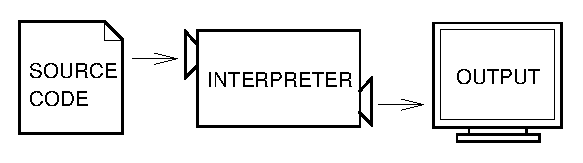
\includegraphics[height=0.77in]{figs/interpret.eps}}
\afterfig

\index{source code}
\index{object code}
\index{executable}

A compiler reads the program and translates it completely before the program 
starts running.  In this context, the high-level program is called the {\bf source 
code}, and the translated program is called the {\bf object code} or the {\bf executable}.  
Once a program is compiled, you can execute it repeatedly without further translation.

\beforefig
\centerline{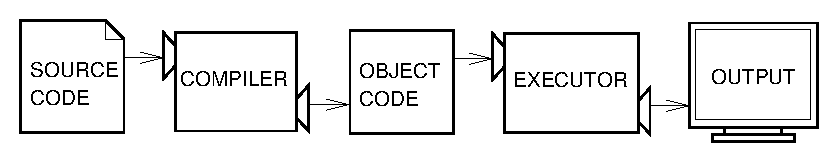
\includegraphics[height=0.77in]{figs/compile.eps}}
\afterfig

One of the nice features of OCaml is that OCaml is both a compiled and an interpreted 
programming language. On the one hand, OCaml can be compiled into an executable file. 
This makes it easier to pass along your program to non-OCaml users, which for a new, 
up-and-coming programming language like OCaml, is a nice feature. On the other hand, 
OCaml can be treated like an interpreted programming language, meaning that an OCaml 
script or OCaml commands can be executed by an interpreter. This is useful for finding 
errors in your code and testing commands and snippits of code. There are two ways to use 
the interpreter: {\bf interactive mode} and {\bf script mode}. In interactive mode, you 
type OCaml commands into the {\bf toplevel} and the interpreter prints the result:

\index{interactive mode}
\index{script mode}

\beforeverb
\begin{verbatim}
# 1+1;;
- : int = 2
\end{verbatim}
\afterverb
%
The octothorp, {\tt \#}, is the {\bf prompt} the interpreter uses to indicate that it is 
ready. The double semi-colons indicates the end of a line. If you type {\tt 1 + 1;;}, the 
interpreter replies {\tt - : int = 2}.

\index{prompt}

Alternatively, you can store code in a file and use the interpreter to execute the contents 
of the file, which is called a {\bf script}.  By convention, OCaml scripts have names that 
end with {\tt .ml}.

\index{script}

\index{testing!interactive mode}

Working in interactive mode is convenient for testing small pieces of code because you can type 
and execute them immediately.  But for anything more than a few lines, you should save your code 
as a script so you can modify and execute it in the future.

\section{The OCaml Toplevel}

Let's take a moment to explain how to use the OCaml toplevel. The toplevel 
works a little differently depending on your operating system. I will cover 
using the toplevel in Windows (7) and Ubuntu (10.04 Karmic). \footnote{Mac users are on their own.}

One thing you will need to use are OCaml commands known as {\bf directives}. 
Directives tell the interpreter or compiler to do specific tasks, like load 
code from a file or exit. A list of some directives  can be found at 
\url{http://caml.inria.fr/pub/docs/manual-ocaml/manual023.html}. 

\index{Directive}
\index{Toplevel}

\subsection{Ubuntu (10.04)}

First off, you must install the ocaml package and its dependencies. Open the terminal and type:

\beforeverb
\begin{verbatim}
 sudo apt-get install ocaml
\end{verbatim}
\afterverb
It will then likely ask you for your admin password. After the installation is complete, you can 
open the OCaml toplevel simply by typing {\tt ocaml} at the command line.

Once in the toplevel, you can open a script by using the {\tt \#use "{\it filename}";;} directive:

\beforeverb
\begin{verbatim}
 #use "myscript.ml";;
\end{verbatim}
\afterverb

Note that the toplevel's {\bf current directory} \footnote{The {\bf current directory} is the 
directory in which ocaml will look to find files to run, outside of the standard ocaml directories.} 
will be the current directory when you ran it within the terminal. You can change your current directory 
using the {\tt \#cd ``{\it dirname}'';;} directive.

\subsection{Windows (7)}

First you must install OCaml. Go to the OCaml home page (\url{caml.inria.fr}) and go to the Download 
page. Download the appropriate distribution - if you don't know which one to choose, go with the 
Windows binary ``for the port based on the Microsoft toolchain.'' Run the installer and follow the 
directions therein.

You can now run an OCaml toplevel from the windows command line by typing {\tt ocaml}. Alternatively,
OCaml has a very pretty toplevel with some nice features which you can open by running "Objective Caml"
from Windows > All Programs > Objective Caml, or open the same program by searching from the windows 
start menu.

Once in the toplevel, you can open a script by using the {\tt \#use "{\it filename}";;} directive:

\beforeverb
\begin{verbatim}
 #use "myscript.ml";;
\end{verbatim}
\afterverb

Note that the toplevel's {\bf current directory} \footnote{The {\bf current directory} is the 
directory in which ocaml will look to find files to run, outside of the standard ocaml directories.} 
will be the current directory when you ran it within the terminal. You can change your current directory 
using the {\tt \#cd ``{\it dirname}'';;} directive.

\section{What is a program?}

A {\bf program} is a sequence of instructions that specifies how to perform a computation.  The computation 
might be something mathematical, such as solving a system of equations or finding the roots of a polynomial, 
but it can also be a symbolic computation, such as searching and replacing text in a document or (strangely 
enough) compiling a program.

\index{program}

The details look different in different languages, but a few basic instructions appear in just about every 
language:

\begin{description}

\item[input:] Get data from the keyboard, a file, or some other device.

\item[output:] Display data on the screen or send data to a file or other device.

\item[math:] Perform basic mathematical operations like addition and multiplication.

\item[conditional execution:] Check for certain conditions and execute the appropriate sequence of statements.

\item[repetition:] Perform some action repeatedly, usually with some variation.

\end{description}

Believe it or not, that's pretty much all there is to it.  Every program you've ever used, no matter how 
complicated, is made up of instructions that look pretty much like these.  So you can think of programming 
as the process of breaking a large, complex task into smaller and smaller subtasks until the subtasks are 
simple enough to be performed with one of these basic instructions.

\index{algorithm}

That may be a little vague, but we will come back to this topic when we talk about {\bf algorithms}.

\section{What is debugging?}
\index{debugging}
\index{bug}

Programming is error-prone.  For whimsical reasons, programming errors are called {\bf bugs}\footnote{It's 
not actually true that it's named after a moth found in a computer relay, though that does make for a rather 
amusing story. For more information on etymology, check out \url{http://en.wikipedia.org/wiki/Software_bug}.} 
and the process of tracking them down is called {\bf debugging}.

\index{debugging}
\index{bug}

Three kinds of errors can occur in a program: syntax errors, runtime errors, and semantic errors. It is useful 
to distinguish between them in order to track them down more quickly.

\subsection{Syntax errors}
\index{syntax error}
\index{error!syntax}
\index{error message}

OCaml can only execute a program if the syntax is correct; otherwise, the interpreter displays an error message.  
{\bf Syntax} refers to the structure of a program and the rules about that structure. For example, parentheses 
have to come in matching pairs, so {\tt (1 + 2)} is legal, but {\tt 8)} is a {\bf syntax error}.

\index{parentheses!matching}
\index{syntax}
\index{cummings, e. e.}

In English readers can tolerate most syntax errors, which is why we can read the poetry of e. e. cummings without 
spewing error messages. OCaml is not so forgiving.  If there is a single syntax error anywhere in your program, 
OCaml will display an error message and quit, and you will not be able to run your program. During the first few 
weeks of your programming career, you will probably spend a lot of time tracking down syntax errors.  As you gain 
experience, you will make fewer errors and find them faster.

\subsection{Runtime errors}
\label{runtime}
\index{runtime error}
\index{error!runtime}
\index{exception}
\index{safe language}
\index{language!safe}

The second type of error is a runtime error, so called because the error does not appear until after the 
program has started running. These errors are also called {\bf exceptions} because they usually indicate 
that something exceptional (and bad) has happened.

Runtime errors are rare in the simple programs you will see in the first few chapters, so it might be a 
while before you encounter one.

\subsection{Semantic errors}
\index{semantics}
\index{semantic error}
\index{error!semantic}
\index{error message}

The third type of error is the {\bf semantic error}.  If there is a semantic error in your program, it will 
run successfully in the sense that the computer will not generate any error messages, but it will not do the 
right thing.  It will do something else.  Specifically, it will do what you told it to do.

The problem is that the program you wrote is not the program you wanted to write.  The meaning of the program 
(its semantics) is wrong. Identifying semantic errors can be tricky because it generally requires you to work 
backward by looking at the output of the program and trying to figure out what it is doing.

\subsection{Experimental debugging}

One of the most important skills you will acquire is debugging. Although it can be frustrating, debugging is one 
of the most intellectually rich, challenging, and interesting parts of programming.

\index{experimental debugging}
\index{debugging!experimental}

In some ways, debugging is like detective work.  You are confronted with clues, and you have to infer the processes 
and events that led to the results you see.

Debugging is also like an experimental science.  Once you have an idea about what is going wrong, you modify your 
program and try again.  If your hypothesis was correct, then you can predict the result of the modification, and 
you take a step closer to a working program.  If your hypothesis was wrong, you have to come up with a new one.  
As Sherlock Holmes pointed out, ``When you have eliminated the impossible, whatever remains, however improbable, 
must be the truth.'' (A. Conan Doyle, {\em The Sign of Four})

\index{Holmes, Sherlock}
\index{Doyle, Arthur Conan}

For some people, programming and debugging are the same thing.  That is, programming is the process of gradually 
debugging a program until it does what you want.  The idea is that you should start with a program that does {\em 
something} and make small modifications, debugging them as you go, so that you always have a working program.

For example, Linux is an operating system that contains thousands of lines of code, but it started out as a simple 
program Linus Torvalds used to explore the Intel 80386 chip.  According to Larry Greenfield, ``One of Linus's 
earlier projects was a program that would switch between printing AAAA and BBBB.  This later evolved to Linux.'' 
({\em The Linux Users' Guide} Beta Version 1).

\index{Linux}

Later chapters will make more suggestions about debugging and other programming practices.

\section{Formal and natural languages}
\index{formal language}
\index{natural language}
\index{language!formal}
\index{language!natural}

{\bf Natural languages} are the languages people speak, such as English, Spanish, and French.  They were not 
designed by people (although people try to impose some order on them); they evolved naturally.

{\bf Formal languages} are languages that are designed by people for specific applications.  For example, the 
notation that mathematicians use is a formal language that is particularly good at denoting relationships 
among numbers and symbols.  Chemists use a formal language to represent the chemical structure of molecules.  
And most importantly:

\begin{quote}
{\bf Programming languages are formal languages that have been designed to express computations.}
\end{quote}

Formal languages tend to have strict rules about syntax.  For example, $3 + 3 = 6$ is a syntactically correct 
mathematical statement, but $3 + = 3 \mbox{\$} 6$ is not.  $H_2O$ is a syntactically correct chemical formula, 
but $_2Zz$ is not.

Syntax rules come in two flavors, pertaining to {\bf tokens} and structure.  Tokens are the basic elements of 
the language, such as words, numbers, and chemical elements.  One of the problems with $3 + = 3 \mbox{\$} 6$ 
is that $\$$ is not a legal token in mathematics (at least as far as I know).  Similarly, $_2Zz$ is not legal 
because there is no element with the abbreviation $Zz$.

\index{token}
\index{structure}

The second type of syntax error pertains to the structure of a statement; that is, the way the tokens are 
arranged.  The statement $3 + = 3 \mbox{\$} 6$ is illegal because even though $+$ and $=$ are legal tokens, 
you can't have one right after the other.  Similarly, in a chemical formula the subscript comes after the 
element name, not before.

\begin{ex}
Write a well-structured English sentence with invalid tokens in it.  Then write another sentence with all 
valid tokens but with invalid structure.
\end{ex}

When you read a sentence in English or a statement in a formal language, you have to figure out what the 
structure of the sentence is (although in a natural language you do this subconsciously).  This process 
is called {\bf parsing}.

\index{parse}

For example, when you hear the sentence, ``The penny dropped,'' you understand that ``the penny'' is the 
subject and ``dropped'' is the predicate.  Once you have parsed a sentence, you can figure out what it 
means, or the semantics of the sentence.  Assuming that you know what a penny is and what it means to 
drop, you will understand the general implication of this sentence.

Although formal and natural languages have many features in common---tokens, structure, syntax, and 
semantics---there are some differences:

\index{ambiguity}
\index{redundancy}
\index{literalness}

\begin{description}

\item[ambiguity:] Natural languages are full of ambiguity, which people deal with by using contextual 
clues and other information. Formal languages are designed to be nearly or completely unambiguous, which 
means that any statement has exactly one meaning, regardless of context.

\item[redundancy:] In order to make up for ambiguity and reduce misunderstandings, natural languages employ 
lots of redundancy.  As a result, they are often verbose.  Formal languages are less redundant and more 
concise.

\item[literalness:] Natural languages are full of idiom and metaphor. If I say, ``The penny dropped,'' 
there is probably no penny and nothing dropping\footnote{This idiom means that someone realized something 
after a period of confusion.}.  Formal languages mean exactly what they say.

\end{description}

People who grow up speaking a natural language---everyone I know---often have a hard time adjusting to 
formal languages.  In some ways, the difference between formal and natural language is like the 
difference between poetry and prose, but more so:

\index{poetry}
\index{prose}

\begin{description}

\item[Poetry:] Words are used for their sounds as well as for their meaning, and the whole poem 
together creates an effect or emotional response.  Ambiguity is not only common but often deliberate.

\item[Prose:] The literal meaning of words is more important, and the structure contributes more 
meaning.  Prose is more amenable to analysis than poetry but still often ambiguous.

\item[Programs:] The meaning of a computer program is unambiguous and literal, and can be understood 
entirely by analysis of the tokens and structure.

\end{description}

Here are some suggestions for reading programs (and other formal languages).  First, remember that 
formal languages are much more dense than natural languages, so it takes longer to read them.  Also, 
the structure is very important, so it is usually not a good idea to read from top to bottom, left 
to right.  Instead, learn to parse the program in your head, identifying the tokens and interpreting 
the structure.  Finally, the details matter.  Small errors in spelling and punctuation, which you can 
get away with in natural languages, can make a big difference in a formal language.

\section{The first program}
\label{hello}

\index{Hello, World}

Traditionally, the first program you write in a new language is called ``Hello, World!'' 
because all it does is display the words, ``Hello, World!''  In Ocaml, one version looks 
like this:

\beforeverb
\begin{verbatim}
print_string ''Hello, World!\n'';;
\end{verbatim}
\afterverb

This is an example of a {\bf print statement}, which doesn't actually print anything on paper. 
It displays a value on the screen.  In this case, the result is:

\beforeverb
\begin{verbatim}
Hello, World!
- : unit = ()
\end{verbatim}
\afterverb

The quotation marks in the program mark the beginning and end of the text to be displayed; they 
don't appear in the result. The ``\\n'' is an {\bf escape character} \footnote{An escape character 
is a special character within a string denoted by a ``whack'' (``\\'') followed by a character or 
series of characters that results in a special character, such as a new line.}, specifically the 
newline character, which tells the output to move to a new line.

\index{escape character}
\index{quotation mark}
\index{print statement}
\index{statement!print}

There's another, more general print statement called ``printf,'' which lets you do more than $print_string$.
Printf comes from it's own {\bf module}, called Printf, meaning you call printf by typing ``Printf.printf.''
Modules are extensions of OCaml that often contain useful functions. Printf is a standard module, meaning
it comes prepackaged with most OCaml installations. You can look up printf on your own if you're interested.

Alternatively, you can import the module by using the \verb"#use" directive:

\beforeverb
\begin{verbatim}
# #use "printf.ml"
\end{verbatim}
\afterverb
%
And then call printf simply as {\tt printf}. However, importing a module generally isn't advised  unless you're
really going to use functions from that module a lot.

\index{module}

Really, we could get simply and just type ``Hello, World!'' and get the result ``{\tt - : string = ''Hello, World!''.}''

Some people judge the quality of a programming language by the simplicity of the ``Hello, World!'' program.  By this 
standard, OCaml does \footnote{Or can do, anyway. There are about as many different OCaml ``Hello, World!'' programs 
as there are OCaml programmers, all arguably equally valid.} about as well as possible.

\section{Functional, as opposed to...?}

\index{Functional Programming}
\index{Programming!Functional}
\index{Programming Paradigms}
\index{Programming Paradigms!Functional}
\index{Programming Paradigms!Object-Oriented}

You may have noticed that this book is entitled ``Think OCaml: How to Think Like a (Functional) Computer Scientist.'' 
No, this is not saying that you'll be good-but-not-great, at programming. Rather, it's a particular paradigm of 
programming. {\bf Functional Programming} is programming where the function is a first-class citizen. Now, this is of 
course a silly definition, but it's the best we can really do for now.
Categorical Abstract Machine Language
Another popular programming paradigm is {\bf Object-Oriented}. Languages that are object-oriented, such as C++ and Python, 
focus rather on having ``objects'' and changing them. ``Object'' is really kind of a blanket term for all kinds of 
different, often custom, ways of storing data.

OCaml is mostly a functional programming language. However, OCaml has support for some level of object-oriented programming,
 unlike it's predecessor Caml. The ``O'' in OCaml stands for ``Objective''.\footnote{``Caml'' once stood for ``Categorical 
Abstract Machine Language'' but it doesn't any more. Now it just represents an even-toed ungulate with humps on its back.}

\section{Debugging}
\index{debugging}

It is a good idea to read this book in front of a computer so you can try out the examples as you go.  You can run most 
of the examples in interactive mode, but if you put the code into a script, it is easier to try out variations.

Whenever you are experimenting with a new feature, you should try to make mistakes.  For example, in the ``Hello, world!'' 
program, what happens if you leave out one of the quotation marks?  What if you leave out both?  What if you spell {\tt 
$print_string$} wrong?

\index{error message}

This kind of experiment helps you remember what you read; it also helps with debugging, because you get to know what the 
error messages mean. It is better to make mistakes now and on purpose than later and accidentally.

Programming, and especially debugging, sometimes brings out strong emotions.  If you are struggling with a difficult bug, 
you might feel angry, despondent or embarrassed.

There is evidence that people naturally respond to computers as if they were people\footnote{See Reeves and Nass, {\it The 
Media Equation: How People Treat Computers, Television, and New Media Like Real People and Places}.}.  When they work well, 
we think of them as teammates, and when they are obstinate or rude, we respond to them the same way we respond to rude, 
obstinate people.

\index{debugging!emotional response}
\index{emotional debugging}

Preparing for these reactions might help you deal with them. One approach is to think of the computer as an employee 
with certain strengths, like speed and precision, and particular weaknesses, like lack of empathy and inability to 
grasp the big picture.

Your job is to be a good manager: find ways to take advantage of the strengths and mitigate the weaknesses.  And 
find ways to use your emotions to engage with the problem, without letting your reactions interfere with your 
ability to work effectively.

Learning to debug can be frustrating, but it is a valuable skill that is useful for many activities beyond 
programming.  At the end of each chapter there is a debugging section, like this one, with my thoughts about 
debugging.  I hope they help!


\section{Glossary}

\begin{description}

\item[problem solving:]  The process of formulating a problem, finding
a solution, and expressing the solution.
\index{problem solving}

\item[high-level language:]  A programming language like OCaml that
is designed to be easy for humans to read and write.
\index{high-level language}

\item[low-level language:]  A programming language that is designed
to be easy for a computer to execute; also called ``machine language'' or
``assembly language.''
\index{low-level language}

\item[portability:]  A property of a program that can run on more
than one kind of computer.
\index{portability}

\item[interpret:]  To execute a program in a high-level language
by translating it one line at a time.
\index{interpret}

\item[compile:]  To translate a program written in a high-level language
into a low-level language all at once, in preparation for later
execution.
\index{compile}

\item[source code:]  A program in a high-level language before
being compiled.
\index{source code}

\item[object code:]  The output of the compiler after it translates
the program.
\index{object code}

\item[executable:]  Another name for object code that is ready
to be executed.
\index{executable}

\item[prompt:] Characters displayed by the interpreter to indicate
that it is ready to take input from the user.
\index{prompt}

\item[script:] A program stored in a file (usually one that will be
interpreted).
\index{script}

\item[interactive mode:] A way of using the Python interpreter by
typing commands and expressions at the prompt.
\index{interactive mode}

\item[script mode:] A way of using the Python interpreter to read
and execute statements in a script.
\index{script mode}

\item[toplevel:] The interface you interact with when working with the interpreter.

\item[program:] A set of instructions that specifies a computation.
\index{program}

\item[algorithm:]  A general process for solving a category of
problems.
\index{algorithm}

\item[bug:]  An error in a program.
\index{bug}

\item[debugging:]  The process of finding and removing any of the
three kinds of programming errors.
\index{debugging}

\item[syntax:]  The structure of a program.
\index{syntax}

\item[syntax error:]  An error in a program that makes it impossible
to parse (and therefore impossible to interpret).
\index{syntax error}

\item[exception:]  An error that is detected while the program is running.
\index{exception}

\item[semantics:]  The meaning of a program.
\index{semantics}

\item[semantic error:]   An error in a program that makes it do something
other than what the programmer intended.
\index{semantic error}

\item[natural language:]  Any one of the languages that people speak that
evolved naturally.
\index{natural language}

\item[formal language:]  Any one of the languages that people have designed
for specific purposes, such as representing mathematical ideas or
computer programs; all programming languages are formal languages.
\index{formal language}

\item[token:]  One of the basic elements of the syntactic structure of
a program, analogous to a word in a natural language.
\index{token}

\item[parse:]  To examine a program and analyze the syntactic structure.
\index{parse}

\item[print statement:]  An instruction that causes the OCaml
interpreter to display a value on the screen.
\index{print statement}
\index{statement!print}


\end{description}


\section{Exercises}

\begin{ex}
Use a web browser to go to the OCaml website \url{caml.inria.fr}.
This page contains information about OCaml (and Caml Light) and links
to OCaml-related pages, and it gives you the ability to search
the Ocaml documentation.

Note that OCaml, like all good things, comes from France (hence the .fr in the url).

\index{documentation}
\index{caml.inria.fr}
\end{ex}

\begin{ex}
 Open the OCaml toplevel and create a ``Hello, World!'' program in interactive mode.

 Now, create a script called ``hello.ml'' that is a ``Hello, World!'' program and run it.

 Experiment with several different methods of writing this program. In particular,
write at least one method using the Printf module. Use the OCaml documentation online to 
understand enough of this module to do so.
\end{ex}


\chapter{Variables and Expressions}

\section{Values and types}
\index{value}
\index{type}
\index{string}

A {\bf value} is one of the basic things a program works with,
like a letter or a number.  Some values we have seen so far
are {\tt 1}, {\tt 2}, and
\verb"'Hello, World!'".

These values belong to different {\bf types}:
{\tt 2} is an integer, and \verb"'Hello, World!'" is a {\bf string},
so-called because it contains a ``string'' of letters.
You (and the interpreter) can identify
strings because they are enclosed in double quotation marks.

\index{quotation mark}

You've already seen \verb"\print_string". There's also a print statement for integers:

\beforeverb
\begin{verbatim}
# print_int 4;;
4- : unit = ()
\end{verbatim}
\afterverb

If you are not sure what type a value has, the interpreter will tell you.

\beforeverb
\begin{verbatim}
# let a = 1;;
val a : int = 1;;
# let foo = "Hello, World!"
val foo : string = "Hello, World!"
\end{verbatim}
\afterverb
%
Not surprisingly, strings belong to the type {\tt string} and
integers belong to the type {\tt int}.  Less obviously, numbers
with a decimal point belong to a type called {\tt float},
because these numbers are represented in a
format called {\bf floating-point}.

\index{type}
\index{string type}
\index{type!str}
\index{int type}
\index{type!int}
\index{float type}
\index{type!float}

\beforeverb
\begin{verbatim}
# let a = 3.2;;
val a : float = 3.2
\end{verbatim}
\afterverb

There's also a separate type called ``char,'' which is short for ``character.'' 
A char is like a string, but it's only one character long (hence the name), and it's surrounded 
by single quotes instead of double quotes. In fact, strings are comprised of lists
of chars. \footnote{A note on pronunciation: most often, ``char'' is pronounced like in charcoal. 
It's less standard, but I personally prefer to pronounce it like it appears in character, since 
that's where it came from.} Usually, you'll use strings, but if you really only need one character, 
chars use less memory.

\index{char type}
\index{type!char}

\beforeverb
\begin{verbatim}
# let foo = 'a';;
val foo : char = 'a'
\end{verbatim}
\afterverb

If you attempt to make a char that's more than one character in length, you get a syntax error:

\beforeverb
\begin{verbatim}
# let foo = 'ab';;
Error: Syntax error
\end{verbatim}
\afterverb

If you enclose a number in quotes, OCaml will infer that it is a char or string, 
depending on the number of quotes.

When you type a large integer, you might be tempted to use commas
between groups of three digits, as in {\tt 1,000,000}.  This is not a
legal integer in OCaml, but it is legal:

\beforeverb
\begin{verbatim}
>>> 1,000,000
- : int * int * int = (1, 0, 0)
\end{verbatim}
\afterverb

Well, that's not what we expected at all!  OCaml interprets {\tt  1,000,000} 
as a comma-separated sequence of integers. Nevermind the type of this object; 
we'll get to it later.

\index{semantic error}
\index{error!semantic}
\index{error message}

This is the first example we have seen of a semantic error: the code
runs without producing an error message, but it doesn't do the
``right'' thing.

There's also one more type, called {\bf unit}, represented as (). This represents 
a sort of ``void''  or ``empty'' value. You'll see where this pops up, and can be useful, later.

\index{type!unit}
\index{unit type}

\section{Variables}
\index{variable}
\index{assignment statement}
\index{statement!assignment}

One of the most powerful features of a programming language is the
ability to manipulate {\bf variables}.  A variable is a name that
refers to a value. In OCaml, variables {\it really} refer to expressions, 
but don't worry about that for now.

An {\bf assignment statement} creates new variables and gives
them values:

\beforeverb
\begin{verbatim}
# let message = "Don't forget to buy milk.";;
val message : string = "Don't forget to buy milk."
# let n = 17;;
val n : int = 17
# let pi = 3.14159265;;
val pi : float = 3.14159265
\end{verbatim}
\afterverb

This example makes three assignments.  The first assigns a string
to a new variable named {\tt message};
the second gives the integer {\tt 17} to {\tt n}; the third
assigns the (approximate) value of $\pi$ to {\tt pi}.

\index{state diagram}
\index{diagram!state}

A common way to represent variables on paper is to write the name with
an arrow pointing to the variable's value.  This kind of figure is
called a {\bf state diagram} because it shows what state each of the
variables is in (think of it as the variable's state of mind).
This diagram shows the result of the previous example:

\beforefig
\centerline{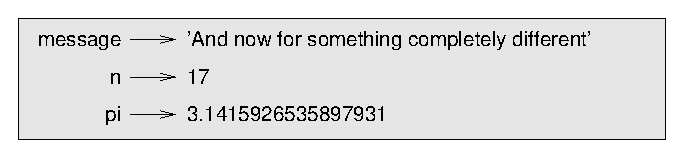
\includegraphics{figs/state2.eps}}
\afterfig

To display the value of a variable, you can simply type it in the toplevel:

\beforeverb
\begin{verbatim}
# n;;
- : int = 17
# pi;;
- : float = 3.14159265
\end{verbatim}
\afterverb

\section{Variable names and keywords}
\index{keyword}

Programmers generally choose names for their variables that
are meaningful---they document what the variable is used for.

Variable names can be arbitrarily long.  They can contain
both letters and numbers, but they have to begin with a letter.
It is legal to use uppercase letters, but it is a good idea
to begin variable names with a lowercase letter (you'll
see why later).

The underscore character (\verb"_") can appear in a name.
It is often used in names with multiple words, such as
\verb"my_name" or \verb"airspeed_of_unladen_swallow", or 
to denote subscripts, such as \verb"y_0" as an initial 
condition. So can an apostraphe (\verb"'"), such as 
\verb"h'".

\index{underscore character}

If you give a variable an illegal name, you get a syntax 
error:

\beforeverb
\begin{verbatim}
# let 17h = 17*17;;
Error: Syntax error
# let more@ = "hello";;
Error: Sytax error
# let class = 2;;
Error: Syntax error
\end{verbatim}
\afterverb

At the toplevel, OCaml will be nice and even underline 
where the error occured for you.

{\tt 7h} is illegal because it does not begin with a letter.
{\tt more@} is illegal because it contains an illegal character, {\tt
@}.  But what's wrong with {\tt class}?

It turns out that {\tt class} is one of OCaml's {\bf keywords}.  The
interpreter uses keywords to recognize the structure of the program,
and they cannot be used as variable names. The full list of keywords 
can be found online here: 
\url{http://caml.inria.fr/pub/docs/manual-ocaml/manual044.html}.

\index{keyword}

You'll get a really interesting error if you try to use just a 
number as a variable:

\beforeverb
\begin{verbatim}
# let 17 = 2;;
Warning P: this pattern-matching is not exhaustive.
Here is an example of a value that is not matched:
0
Exception: Match_failure ("", 8, -17).
\end{verbatim}
\afterverb

That's fun. Technically, this is a semantic error causing a 
syntax error. This will make a little more sense later when
we talk about pattern-matching.

\section{Operators and operands}
\index{operator, arithmetic}
\index{arithmetic operator}
\index{operand}
\index{expression}

{\bf Operators} are special symbols that represent computations like
addition and multiplication.  The values the operator is applied to
are called {\bf operands}.

\index{operator}

In OCaml, operators are {\bf strictly typed}, meaning you can't use an integer operator
for a float, or vice versa. OCaml, unlike some other programming languages, won't
even infer that you meant a float when you put an int, or vice versa. This can make
debugging type errors much simpler, though it seems like a pain at first.

\index{Strictly typed}

For integers, the operators {\tt +}, {\tt -}, {\tt *}, and {\tt /}
perform addition, subtraction, multiplication, and division, as in 
the following examples:

\beforeverb
\begin{verbatim}
20+32   hour-1   hour*60+minute   minute/60  (5+9)*(15-7)
\end{verbatim}
\afterverb

For floating-points, the operators are the same, but followed by a period, namely 
{\tt +.}, {\tt -.}, {\tt *.}, and {\tt /.}. There is also a floating point operator for
exponentiation, namely {\tt **}. There is no integer exponention, probably because an integer
raised to a negative integer would result in a non-integer. \footnote{This is not to say that 
a function can't take two integers and return a float.}

In some other languages, \verb"^" is used for exponentiation, but
in OCaml it is used for string concatenation, meaning the two strings 
are added end-to-start, such as in the following example:

\beforeverb
\begin{verbatim}
 # "Hello, "^"World!";;
- : string = "Hello, World!"
\end{verbatim}
\afterverb

Don't forget to put a space somewhere so your words are separated 
when you concatenate.

You can change an int to a float or vice versa using the 
OCaml functions \verb"float_of_int" or \verb"int_of_float", like so:

\beforeverb
\begin{verbatim}
 float_of_int x;; int_of_float x;;
\end{verbatim}
\afterverb

I'll leave determining which is which as an exercise to the reader.

\section{Expressions}

An {\bf expression} is a combination of values, variables, operators
and functions that returns a particular value. A value all by itself 
is an expression, and so is a variable, so the following are all legal 
expressions (assuming that the variable {\tt x} has been assigned a value):

\index{expression}
\index{evaluate}

\beforeverb
\begin{verbatim}
17;;
x;;
x + 17;;
\end{verbatim}
\afterverb
%
If you type an expression in interactive mode, the interpreter
{\bf evaluates} it and displays the result:

\beforeverb
\begin{verbatim}
# 1 + 1;;
- : int = 2
\end{verbatim}
\afterverb

\index{subexpressions}
Expressions can, and often do,\footnote{Any expression with more than just a value or 
variable technically contains subexpressions.} contain other expressions, called {\bf 
subexpressions}. When evaluating the value of the expression, the OCaml interpreter 
will evaluate the embedded expression and substitute it in to the larger expression. 
In OCaml, and many other function-oriented languages, everything must be an expression. 
Everything up to a double semi-colon ({\tt ;;}) must be exactly one expression, with 
arbitrarily many sub-expressions.

\begin{ex}
Type the following statements in the OCaml interpreter to see
what they do:

\beforeverb
\begin{verbatim}
5;;
let x = 5;;
x + 1;;
\end{verbatim}
\afterverb
%
Now put the same statements into a script and run it.  What
is the output?
\end{ex}

\section{Variables as Expressions, and References}

\index{Variables!References}
\index{References}

Now, this is where I admit that I lied to you a little bit.

Remember how I said that the expression ``let x = 3;;'' assigns
the values of `3' to the variable `x'? Well, that's not
entirely true. In fact, it's not true at all.

What really happens when I say ``let x = 3;;'' is that the {\it expression}
`3' is represented by `x'. `x' becomes kind of a shorthand way of writing `3'.

One of the side effects of this is that you can't change the value of a variable.
So, really, in some sense, they shouldn't be called variables at all.

\section{Scope}

Now, I said you couldn't change the value of variables, but in some senses it looks like you can.

\index{Scope}

\beforeverb
\begin{verbatim}
 # let x = 2;;
val x : int = 2
 # let x = 3;;
val x : int = 3;;
 # x;;
- : x = 3
\end{verbatim}
\afterverb

See? The value of `x' changed! Didn't it?

\index{scope}
Actually, the answer is no, it didn't. What we have here is a problem of {\bf scope}. You see, variables
all act within certain bounds, or on certain levels within a program. Every time we say ``let'', it kind of
creates a new ``level'' of the program, within which only certain variables can be accessed. This brings up
let's counterpart, `in'. The best way to explain `in' is with an example.

\beforeverb
\begin{verbatim}
 # let x = 2;;
val x : int = 2
 # let x = 3 in x+1;;
- : int = 4
 # x;;
- : int = 2
\end{verbatim}
\afterverb

Now, didn't see that last bit coming, did you? When you use ``let... in...;;'', the value assigned by the let only
exists within the expression after in. This is called a ``let-in-binding''.

\index{let}
\index{in}

\begin{ex}
 Play around with scope a little bit in the command line.

 See if you can predict the outcome of the following:
 
 \newcounter{exno}
\begin{list}{\arabic{exno}}{}
  \item
 \beforeverb
 \begin{verbatim}
  # let x = 2 in x+1;;
  # let x = 3 in x+1;;
  # x;;
 \end{verbatim}
 \afterverb
   \item 
 \beforeverb
 \begin{verbatim}
  # let x = 2;;
  # let y = 3 in let x = 2 in x+y;;
  # x;;
  # y;;
 \end{verbatim}
 \afterverb
\end{list}

Now try them out in the interpreter and see if you were right!
\end{ex}


\section{Order of operations}
\index{order of operations}
\index{rules of precedence}
\index{PEMDAS}

When more than one operator appears in an expression, the order of
evaluation depends on the {\bf rules of precedence}.  For
mathematical operators, OCaml follows mathematical convention.
The acronym {\bf PEMDAS} is a useful way to
remember the rules:

\index{parentheses!overriding precedence}

\begin{itemize}

\item {\bf P}arentheses have the highest precedence and can be used 
to force an expression to evaluate in the order you want. Since
expressions in parentheses are evaluated first, {\tt 2 * (3-1)} is 4,
and {\tt (1.+.1.)**(5.-.2.)} is 8.. You can also use parentheses to make an
expression easier to read, as in {\tt (minute * 100) / 60}, even
if it doesn't change the result.

\item {\bf E}xponentiation has the next highest precedence, so
{\tt 2.**1.+.1.} is 3., not 4., and {\tt 3.*1.**3.} is 3., not 27..

\item {\bf M}ultiplication and {\bf D}ivision have the same precedence,
which is higher than {\bf A}ddition and {\bf S}ubtraction, which also
have the same precedence.  So {\tt 2*3-1} is 5, not 4, and
{\tt 6+4/2} is 8, not 5.

\item Operators with the same precedence are evaluated from left to 
right.  So in the expression {\tt degrees /. 2. * pi}, the division
happens first and the result is multiplied by {\tt pi}.  
To divide by $2 \pi$, you can use parentheses or write {\tt degrees /. 2. /. pi}.

\end{itemize}

Technically speaking, all operations in the programming language follow some sort
of order of operations. However, you don't really need to know more than that 
parentheses override all that precedence. In fact, if you need to know more about
the order of operations than the above mathematical rules, then you're not making
your code clear enough and should use parentheses to make things more clear.

\section{String operations}
\index{string!operation}
\index{operator!string}

You cannot perform mathematical operations on strings, even
if the strings look like numbers, so the following are illegal:

\beforeverb
\begin{verbatim}
"2"-"1"    "eggs"/"easy"    "third"*"a charm"  "you"+"me"
\end{verbatim}
\afterverb

In OCaml, an operator cannot be used for two things. In some languages,
for example Python, operators can be {\bf overloaded}, meaning they do different
things in different situations (i.e., `+' can be used for string concatenation).
In OCaml, this is not the case.

\index{operator!overloading}

\section{Comments}
\index{comment}

As programs get bigger and more complicated, they get more difficult
to read.  Formal languages are dense, and it is often difficult to
look at a piece of code and figure out what it is doing, or why.

For this reason, it is a good idea to add notes to your programs to explain
in natural language what the program is doing.  These notes are called
{\bf comments}, and they start with a \verb"(*" and end with a \verb"*)":

\beforeverb
\begin{verbatim}
(* compute the percentage of the hour that has elapsed *)
percentage = (minute * 100) / 60
\end{verbatim}
\afterverb

Everything between the parentheses will be ignored by the compiler. 
You can also put comments at the end, or even in the middle, of a 
line of code:

\beforeverb
\begin{verbatim}
 # let x = 2;; (* I'm a comment! *)
val x : int = 2
 # let x (* Hi, mom! *) = 3;;
val x = 3
\end{verbatim}
\afterverb

Of course, putting comments in the middle of expressions like that can be really 
annoying to read.

Comments are most useful when they document non-obvious features of
the code.  It is reasonable to assume that the reader can figure out
{\em what} the code does; it is much more useful to explain {\em why}.

This comment is redundant with the code and useless:

\beforeverb
\begin{verbatim}
let v = 5;;     (* assign 5 to v *)
\end{verbatim}
\afterverb
%
This comment contains useful information that is not in the code:

\beforeverb
\begin{verbatim}
let v = 5;;     (* velocity in meters/second. *)
\end{verbatim}
\afterverb
%
Good variable names can reduce the need for comments, but
long names can make complex expressions hard to read, so there is
a tradeoff.

\section{Debugging}
\index{debugging}

At this point the syntax error you are most likely to make is
an illegal variable name, like {\tt class}, which
is a keyword, or \verb"odd.job" and \verb"hack_and_/", which contain
illegal characters.

\index{syntax error}
\index{error!syntax}

For syntax errors, the error messages don't help much.
The most common message is {\tt SyntaxError: invalid 
syntax} which is not very informative.

\index{error message}
\index{use before def}
\index{exception}
\index{runtime error}
\index{error!runtime}

The runtime error you are most likely to make is a ``unbound value'' that is,
trying to use a variable before you have assigned
a value.  This can happen if you spell a variable name wrong:

\beforeverb
\begin{verbatim}
 # let principal = 327.68;;
val principal : float = 327.68
 # let interest = principle *. rate;;
Error: Unbound value principle
\end{verbatim}
\afterverb

Variables names are case sensitive, so {\tt LaTeX} is not the
same as {\tt latex}.

\index{case-sensitivity, variable names}
\index{semantic error}
\index{error!semantic}

At this point the most likely cause of a semantic error is
the order of operations.  For example, to evaluate $\frac{1}{2 \pi}$,
you might be tempted to write

\beforeverb
\begin{verbatim}
 # 1. /. 2. *. pi;;
\end{verbatim}
\afterverb
%
But the division happens first, so you would get $\pi / 2$, which
is not the same thing!  There is no way for OCaml
to know what you meant to write, so in this case you don't
get an error message; you just get the wrong answer.

\index{order of operations}

Another semantic error you might encounter is a scope error.
For example, assigning a variable for one scope and trying to use it
in another:

\beforeverb
\begin{verbatim}
 # let devil = -1;;
val a : int = -1
 # let god = 1 in god+devil;;
- : int = 0;;
 # god+devil;;
Error: unbound value god
\end{verbatim}
\afterverb

The last common semantic error I'll mention now is attempting to create
a variable name with a space in it, which OCaml interprets as a function
definition:

\beforeverb
\begin{verbatim}
# let bad name = 5;;
val bad : 'a -> int = <fun>
# bad 2;;
- : int = 4
# bad "Please, anything but 4!";;
- : int = 4
\end{verbatim}
\afterverb

What you've done is written a function {\tt bad} that takes one argument of 
any type and always returns {\tt 4}. This will make more sense when we see 
functions next chapter.

\section{Glossary}

\begin{description}

\item[value:]  One of the basic units of data, like a number or string, 
that a program manipulates.
\index{value}

\item[type:] A category of values.  The types we have seen so far
are integers (type {\tt int}), floating-point numbers (type {\tt
float}), strings (type {\tt str}), characters (type {\tt char}), and 
the unit type (type {\tt unit}, {\tt ()}).
\index{type}

\item[integer:] A type that represents whole numbers.
\index{integer}

\item[floating-point:] A type that represents numbers with fractional
parts.
\index{floating-point}

\item[string:] A type that represents sequences of characters.
\index{string}

\item[character: ] A type that represents a single character.
\index{character}

\item[unit type: ] A null or empty type.
\index{unit type}

\item[variable:]  A name that refers to a value. Actually, acts as shorthand for an expression.
\index{variable}

\item[statement:]  A section of code that represents a command or action.  So
far, the statements we have seen are assignments and print statements.
\index{statement}

\item[assignment:]  A statement that assigns a value to a variable.
\index{assignment}

\item[state diagram:]  A graphical representation of a set of variables and the
expressions they refer to.
\index{state diagram}

\item[keyword:]  A reserved word that is used by the compiler to parse a
program; you cannot use keywords like {\tt if}, {\tt  class}, and {\tt while} as
variable names.
\index{keyword}

\item[operator:]  A special symbol that represents a simple computation like
addition, multiplication, or string concatenation.
\index{operator}

\item[operand:]  One of the values on which an operator operates.
\index{operand}

\item[expression:]  A combination of variables, operators, and values that
represents a single result value.
\index{expression}

\item[evaluate:]  To simplify an expression by performing the operations
in order to yield a single value.

\item[rules of precedence:]  The set of rules governing the order in which
expressions involving multiple operators and operands are evaluated.
\index{rules of precedence}
\index{precedence}

\item[concatenate:]  To join two operands end-to-end.
\index{concatenation}

\item[comment:]  Information in a program that is meant for other
programmers (or anyone reading the source code) and has no effect on the
execution of the program.
\index{comment}

\end{description}


\section{Exercises}

\begin{ex}
Assume that we execute the following assignment statements:

\begin{verbatim}
let width = 17;;
let height = 12.0;;
let delimiter = '.';;
\end{verbatim}

For each of the following expressions, write the value of the
expression and the type (of the value of the expression).

\begin{enumerate}

\item {\tt width/2}

\item {\tt width/.2.0}

\item {\tt height/3}

\item {\tt 1 + 2 * 5}

\item {\tt delimiter * 5}

\end{enumerate}

Use the OCaml interpreter to check your answers.
\end{ex}

\begin{ex}
Practice using the OCaml interpreter as a calculator: 
\index{calculator}

\begin{enumerate}

\item The volume of a sphere with radius $r$ is $\frac{4}{3} \pi r^3$.
  What is the volume of a sphere with radius 5?  Hint: 392.6 is wrong!

\item Suppose the cover price of a book is \$24.95, but bookstores get a
  40\% discount.  Shipping costs \$3 for the first copy and 75 cents
  for each additional copy.  What is the total wholesale cost for
  60 copies?

\item If I leave my house at 6:52 am and run 1 mile at an easy pace
  (8:15 per mile), then 3 miles at tempo (7:12 per mile) and 1 mile at
  easy pace again, what time do I get home for breakfast?

\index{running pace}

\end{enumerate}
\end{ex}

\chapter{Functions}
\label{funcchap}

\section{Function calls}
\label{functionchap}
\index{function call}

In the context of functional programming, a {\bf function} is a named 
expression that performs a computation.  When you define a function,
you specify the name and the expression.  Later, you can ``call'' the 
function by name.  We have already seen one example of a {\bf function 
call}:

\beforeverb
\begin{verbatim}
# float_of_int 32;;
- : float = 32.
\end{verbatim}
\afterverb
%
The name of the function is {\tt \verb"float_of_int"}.  The expression that follows
is called the {\bf argument} of the function.  The result, for this
function, is a floating-point version of the integer argument. There is, of course, the
inverse function,\verb"int_of_float". There are other type conversion functions, too, such as
\verb"string_of_int" and \verb"string_of_float" and their respective inverses.

It is common to say that a function ``takes'' an argument and ``returns''
a result.  The result is called the {\bf return value}.

\index{argument}
\index{return value}

\section{Math functions}
\index{math function}
\index{function, math}

OCaml provides most of the familiar mathematical functions, including
the trig functions and their inverses, log (natural log) and base-10 log.
Naturally, they all take float arguments, not integers.

\beforeverb
\begin{verbatim}
# let ratio = signal_power /. noise_power;
# decibels = 10. *. log10 ratio;;

# radians = 0.7;;
# height = sin radians;;
\end{verbatim}
\afterverb
%
The first example computes the base-10 logarithm of the
signal-to-noise ratio.

\index{log function}
\index{function!log}
\index{sine function}
\index{radian}
\index{trigonometric function}
\index{function, trigonometric}

The second example finds the sine of {\tt radians}.  The name of the
variable is a hint that {\tt sin} and the other trigonometric
functions ({\tt cos}, {\tt tan}, etc.)  take arguments in radians. To
convert from degrees to radians, divide by 360 and multiply by $2
\pi$:

\beforeverb
\begin{verbatim}
# let degrees = 45.;;
# let pi = 4. *. atan 1.0;;
# let radians = degrees /. 360. *. 2. *. pi;;
# sin radians;;
0.707106781187
\end{verbatim}
\afterverb
%

If you know
your trigonometry, you can check the previous result by comparing it to
the square root of two divided by two:

\index{sqrt function}
\index{function!sqrt}

\beforeverb
\begin{verbatim}
# (sqrt 2.) /. 2.0
0.707106781187
\end{verbatim}
\afterverb

\section{Composition}
\index{composition}

So far, we have looked at the elements of a program---variables,
expressions, and statements---in isolation, without talking about how to
combine them.

One of the most useful features of programming languages is their
ability to take small building blocks and {\bf compose} them.  For
example, the argument of a function can be any kind of expression,
including arithmetic operators:

\beforeverb
\begin{verbatim}
let x = sin (degrees /. 360.0 *. 2 *. pi);;
\end{verbatim}
\afterverb
%
And even function calls:t

\beforeverb
\begin{verbatim}
let x = exp (log (x+.1.));;
\end{verbatim}
\afterverb
%
Note in this example that we put parentheses around the inner function and the inner 
expression, to tell OCaml how to read this statement. If we just told it \verb"exp log x+1;;" it would try to pass both {\tt log} and {\tt x} as two separate arguments 
to {\tt exp} and then add one.

Almost anywhere you can put a value, you can put an arbitrary
expression, with one exception: the left side of an assignment
statement has to be a variable name, or function definition, which
you'll see in the next section.  Any other expression on the left
side is a syntax error.

\beforeverb
\begin{verbatim}
 # let minutes = hours *. 60.0;;                 (* right *)
 # let hours *. 60 = minutes;;;                  (* wrong! *)
Error: Syntax error
\end{verbatim}
\afterverb
%
\index{SyntaxError}
\index{exception!SyntaxError}


\section{Adding new functions}

So far, we have only been using the functions that come with OCaml,
but it is also possible to add new functions.
A {\bf function definition} specifies the name of a new function and
the sequence of statements that execute when the function is called.

\index{function}
\index{function definition}
\index{definition!function}

Here is an example:
%edit here

\beforeverb
\begin{verbatim}
let  print_lyrics () = 
    print_string "I'm a lumberjack, and I'm okay. \n";
    print_string "I sleep all night and I work all day. \n";;
\end{verbatim}
\afterverb
%
Note that we use the "let" keyord to define functions just the same as
variables. The name of the function is \verb"print_lyrics".  The
rules for function names are the same as for variable names: letters,
numbers and some punctuation marks are legal, but the first character
can't be a number.  You can't use a keyword as the name of a function,
and you should avoid having a variable and a function with the same
name.

\index{argument}

The empty parentheses after the name indicate that this function
doesn't take any meaningful arguments. More specifically, it takes a unit type
argument, meaning when we call it we have to put empty parentheses after it.
If we don't put the parentheses, then it gives us a little information about
the function:

\beforeverb
\begin{verbatim}
# print_lyrics;;
- : unit -> unit = <fun>
\end{verbatim}
\afterverb
What this output means is that this is a function (\verb" = <fun>") which takes
a unit type argument and returns a unit (\verb"unit -> unit"). We'll see why this
is useful later.

But wait! Was that a single semi-colon I saw there? What was that? I thought
you used two semi-colons to end a statement? Well, sure, two semi-colons do
end a statement. But if you put two semi-colons inside a function definition, 
that ends the entire function definiton. So if we want a function to execute
one statement and then execute another statement, we terminate all the intermediate
statements with single semi-colons, which is called a {\em sequence point}. \footnote{
The sequence point is actually an operator, like +. It takes a unit on the 
left and anything on the right and returns the right.}
If we don't, we get an interesting syntax error:

\beforeverb
\begin{verbatim}
# let print_lyrics () = 
	print_string "I'm a lumberjack and I'm okay. \n"
	print_string "I work all night and I sleep all day. \n";;
Error: This function is applied to too many arguments;
maybe you forgot a `;'
\end{verbatim}
\afterverb
It's trying to treat the second \verb"print_string" as another argument in the first \verb"print_string"!
That's because we didn't give it anything to tell it that we've stopped putting in arguments
to the first \verb"print_string". In OCaml, a new line in code is nothing more than a space.
New lines and indentation just make your code easier to read and more organized. It doesn't
help the  OCaml compiler at all.

\index{parentheses!empty}
\index{type!unit}
\index{unit type}
\index{header}
\index{body}

The syntax for calling the new function is the same as for built-in functions:

\beforeverb
\begin{verbatim}
# print_lyrics();;
I'm a lumberjack, and I'm okay.
I sleep all night and I work all day.
- : unit = ()
\end{verbatim}
\afterverb
%
Once you have defined a function, you can use it inside another
function.  For example, to repeat the previous refrain, we could write
a function called \verb"repeat_lyrics":

\beforeverb
\begin{verbatim}
let repeat_lyrics() = 
    print_lyrics();
    print_lyrics();;
\end{verbatim}
\afterverb
%
And then call \verb"repeat_lyrics();;":

\beforeverb
\begin{verbatim}
# repeat_lyrics()
I'm a lumberjack, and I'm okay.
I sleep all night and I work all day.
I'm a lumberjack, and I'm okay.
I sleep all night and I work all day.
- : unit = ()
\end{verbatim}
\afterverb
%
But that's not really how the song goes.


\section{Definitions and uses}
\index{function definition}

Pulling together the code fragments from the previous section, the
whole program looks like this:

\beforeverb
\begin{verbatim}
let print_lyrics() =
    print_string "I'm a lumberjack, and I'm okay. \n";
    print_string "I sleep all night and I work all day. \n";;

let repeat_lyrics() =
    print_lyrics();
    print_lyrics();;

repeat_lyrics()
\end{verbatim}
\afterverb
%
This program contains two function definitions: \verb"print_lyrics" and
\verb"repeat_lyrics".  Function definitions get executed just like other
statements, but the effect is to create functions.  The statements
inside the function do not get executed until the function is called, and
the function definition generates only trivial output.

In OCaml, so you can define a function after you call it, so long as it is 
called and defined in the same script.

\begin{ex}
Move the last line of this program
to the top, so the function call appears before the definitions. Run 
the program and see if the output changes.
\end{ex}

\begin{ex}
Move the function call back to the bottom
and move the definition of \verb"print_lyrics" after the definition of
\verb"repeat_lyrics".  What happens when you run this program?
\end{ex}


\section{Flow of execution}
\index{flow of execution}

Execution always begins at the first statement of the program.
Statements are executed one at a time, in order from top to bottom.

Function definitions do not alter the flow of execution of the
program, but remember that statements inside the function are not
executed until the function is called.

A function call is like a detour in the flow of execution. Instead of
going to the next statement, the flow jumps to the body of
the function, executes all the statements there, and then comes back
to pick up where it left off.

That sounds simple enough, until you remember that one function can
call another.  While in the middle of one function, the program might
have to execute the statements in another function. But while
executing that new function, the program might have to execute yet
another function!

Fortunately, OCaml is good at keeping track of where it is, so each
time a function completes, the program picks up where it left off in
the function that called it.  When it gets to the end of the program,
it terminates.

What's the moral of this sordid tale?  When you read a program, you
don't always want to read from top to bottom.  Sometimes it makes
more sense if you follow the flow of execution.


\section{Parameters and arguments}
\label{parameters}
\index{parameter}
\index{function parameter}
\index{argument}
\index{function argument}

Some of the built-in functions we have seen require arguments.  For
example, when you call {\tt sin} you pass a floating-point
as an argument.  Some functions take more than one argument.

Inside the function, the arguments are assigned to
variables called {\bf parameters}.  Here is an example of a
user-defined function that takes an argument:

\index{parentheses!parameters in}

\beforeverb
\begin{verbatim}
let print_twice bruce =
	print_int bruce;
	print_string " ";
	print_int bruce;
	print_string "\n";;
\end{verbatim}
\afterverb
%
This function assigns the argument to a parameter
named {\tt bruce}.  When the function is called, it prints the value of
the parameter (which must be an integer) twice, with a space in between then
followed by a new line.

The same rules of composition that apply to built-in functions also
apply to user-defined functions, so we can use any kind of expression
as an argument for \verb"print_twice", so long as it evaluates to an integer:

\index{composition}

\beforeverb
\begin{verbatim}
>>> print_twice (3*4)
12 12
- : unit = ()
>>> print_twice (2+10)
12 12
- : unit = ()
\end{verbatim}
\afterverb
%
Note that we need to tell OCaml exactly what the argument is using parentheses in this case.
This is because if we omitted them it would read left to right, so the first function call 
would become {\tt (\verb"print_twice" 3)*4}, which doesn't make any sense, especially since
{\tt (\verb"print_twice" 3)} evaluates to a unit, which you can't really multiply by four.

The argument is evaluated before the function is called, so
in the examples the expressions {\tt 3*4} and
{\tt 2+10} are only evaluated once.

\index{argument}

You can also use a variable as an argument:

\beforeverb
\begin{verbatim}
>>> michael = 1
>>> print_twice michael
1 1
- : unit = ()
\end{verbatim}
\afterverb
%
The name of the variable we pass as an argument ({\tt michael}) has
nothing to do with the name of the parameter ({\tt bruce}).  It
doesn't matter what the value was called back home (in the caller);
here in \verb"print_twice", we call everybody {\tt bruce}.

\index{Higher-Order Functions}
\index{HOF}

Functions can also take other functions as arguments. Such a function
is called a {\em Higher-Order Function}, which is sometimes abbreviated HOF.


\section{Functions are Just Renamed Expressions}

In OCaml, functions are really just expressions renamed. This means that an 
Ocaml function must evaluate to a value, hence why you must use sequence points 
within a function definition.

Using {\tt let} within a function definition requires the in keyword:

\index{concatenation}

\beforeverb
\begin{verbatim}
let cat_twice part1 part2 = 
    let cat = part1^part2^"\n" in cat^cat;;
\end{verbatim}
\afterverb
This function takes two string arguments, concatenates them and adds a newline character, 
and then concatenates the result to itself and returns this string. Note that ``in'' in there: that's
so that the variable definition doesn't return anything itself; it's only part of an expression which
returns the result.

\section{Scope and Functions}
\index{local variable}
\index{variable!local}


\beforeverb
\begin{verbatim}
# let line1 = 'Bing tiddle ';;
# let line2 = 'tiddle bang.';;
# cat_twice line1 line2;;
Bing tiddle tiddle bang.
- : unit = ()
\end{verbatim}
\afterverb

When \verb"cat_twice" terminates, the variable {\tt cat}
is destroyed.  If we try to print it, we get an exception:

\beforeverb
\begin{verbatim}
# print_string cat
Error: Unbound value cat
\end{verbatim}
\afterverb

Parameters are also local.
For example, outside \verb"_twice", there is no
such thing as {\tt bruce}.

\index{parameter}


\section{Stack diagrams}
\label{stackdiagram}
\index{stack diagram}
\index{function frame}
\index{frame}
%edit here like a mofo!
To keep track of which variables can be used where, it is sometimes 
useful to draw a {\bf stack diagram}.  Like state diagrams, stack 
diagrams show the value of each variable, but they also show the 
function each variable belongs to.

\index{stack diagram}
\index{diagram!stack}

Each function is represented by a {\bf frame}.  A frame is a box
with the name of a function
beside it and the parameters and variables of the function inside it.
The stack diagram for the
previous example looks like this:

\beforefig
\centerline{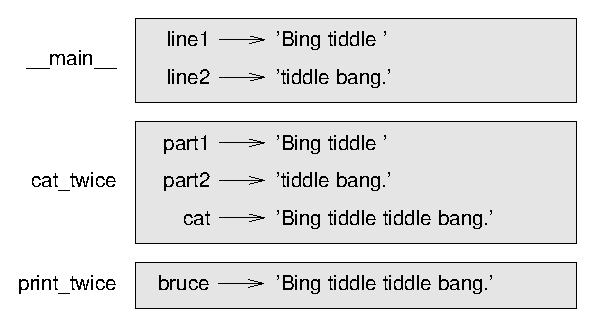
\includegraphics{figs/stack.eps}}
\afterfig

The frames are arranged in a stack that indicates which function
called which, and so on.  In this example, \verb"print_twice"
was called by \verb"cat_twice", and \verb"cat_twice" was called by 
\verb"__main__", which is a special name for the topmost frame.  When
you create a variable outside of any function, it belongs to 
\verb"__main__".

Each parameter refers to the same value as its corresponding
argument.  So, {\tt part1} has the same value as
{\tt line1}, {\tt part2} has the same value as {\tt line2},
and {\tt bruce} has the same value as {\tt cat}.

\section{Currying Functions}

\index{Currying}
\index{Functions!Currying}

Currying functions is a very odd, but very powerful, idea in OCaml.

You've probably noticed that OCaml gives you a very interesting output
after a function definition. Consider the following (somewhat trivial) function:

\beforeverb
\begin{verbatim}
# let add a b = a+b;;
val add: int -> int -> int = <fun>
\end{verbatim}
\afterverb

Effectively, what this means is that you have a function which takes two 
integers as input and returns an integer (in this case, the sum of the two). 
What's with the arrows, then? Well, this syntax was chosen for a reason.

Consider the following:

\beforeverb
\begin{verbatim}
# add 3;;
\end{verbatim}
\afterverb

What is that? If you're familiar with other programming languages, you might 
assume it's a syntax error: the function doesn't have enough input arguments!
Well, you would be wrong. In fact, there's no error at all. That is a perfectly
valid statement in OCaml:

\beforeverb
\begin{verbatim}
# add 3;;
- : int -> int = <fun>
\end{verbatim}
\afterverb

That's right, {\tt add 3} is actually a function in it's own right. It takes an integer
as an input, to which it will add three and then return the result. That's because functions
of multiple input arguments in OCaml are really just chains of single-argument functions. 
Hence, {\tt add a b} is really the function {\tt add a} applied to {\tt b}, which is really 
the function {\tt add} applied to {\tt a}, the result of which is then applied to {\tt b}. 
\footnote{If you've never heard of currying before and that made sense to you the first 
time through, then you deserve a medal and you're going to love when we get to recursion.} 
This is called `{\bf currying}, after Haskell Curry. It is also sometimes called 
{\bf partial application}.

\index{Partial Application}

In fact, we can even name this function:

\beforeverb
\begin{verbatim}
# let add3 = add 3;;
val add3 : int -> int = <fun>
# add3 2;;
- : int = 5
\end{verbatim}
\afterverb

This would be effectively the same as writing:

\beforeverb
\begin{verbatim}
# let add3 b = add 3 b;;
val add3 : int -> int = <fun>
# add3 2;;
- : int = 5
\end{verbatim}
\afterverb
%
Except the first one is a little cleaner. In this trivial example, the difference is
very slight, but when we introduce some new concepts later, you'll see why currying
is so powerful.

\section{Why functions?}
\index{function, reasons for}

It may not be clear why it is worth the trouble to divide
a program into functions.  There are several reasons:

\begin{itemize}

\item Creating a new function gives you an opportunity to name a group
of statements, which makes your program easier to read and debug.

\item Functions can make a program smaller by eliminating repetitive
code.  Later, if you make a change, you only have
to make it in one place.

\item Dividing a long program into functions allows you to debug the
parts one at a time and then assemble them into a working whole.

\item Well-designed functions are often useful for many programs.
Once you write and debug one, you can reuse it.

\end{itemize}

\section{Debugging}
\label{editor}
\index{debugging}

Don't forget to save your program before you run it.  Some
development environments do this automatically, but some don't.
In that case the program you are looking at in the text editor
is not the same as the program you are running.

Debugging can take a long time if you keep running the same,
incorrect, program over and over!

Make sure that the code you are looking at is the code you are running.
If you're not sure, put something like {\verb print_int 42} at the
beginning of the program and run it again.  If you don't see
{\tt 42}, you're not running the right program!


\section{Glossary}

\begin{description}

\item[function:] A named sequence of statements that performs some
useful operation.  Functions may take any parameter and return any 
type, including the unit type.
\index{function}

\item[function definition:]  A statement that creates a new function,
specifying its name, parameters, and the statements it executes.
\index{function definition}

\item[function object:]  A value created by a function definition.
The name of the function is a variable that refers to a function
object.
\index{function definition}

\item[header:] The first line of a function definition.
\index{header}

\item[body:] The sequence of statements inside a function definition.
\index{body}

\item[parameter:] A name used inside a function to refer to the value
passed as an argument.
\index{parameter}

\item[function call:] A statement that executes a function. It
consists of the function name followed by an argument list.
\index{function call}

\item[argument:]  A value provided to a function when the function is called.
This value is assigned to the corresponding parameter in the function.
\index{argument}

\item[local variable:]  A variable defined inside a function.  A local
variable can only be used inside its function.
\index{local variable}

\item[return value:]  The result of a function.  If a function call
is used as an expression, the return value is the value of
the expression.
\index{return value}

%\item[fruitful function:] A function that returns a value.
%\index{fruitful function}

%\item[void function:] A function that doesn't return a value.
%\index{void function}

\item[module:] A file that contains a
collection of related functions and other definitions.
\index{module}

%\item[import statement:] A statement that reads a module file and creates
%a module object.
%\index{import statement}
%\index{statement!import}

%\item[module object:] A value created by an {\tt import} statement
%that provides access to the values defined in a module.
%\index{module}

\item[dot notation:]  The syntax for calling a function in another
module by specifying the module name followed by a dot (period) and
the function name.
\index{dot notation}

\item[composition:] Using an expression as part of a larger expression,
or a statement as part of a larger statement.
\index{composition}

\item[flow of execution:]  The order in which statements are executed during
a program run.
\index{flow of execution}

%\item[stack diagram:]  A graphical representation of a stack of functions,
%their variables, and the values they refer to.
%\index{stack diagram}

%\item[frame:]  A box in a stack diagram that represents a function call.
%It contains the local variables and parameters of the function.
%\index{function frame}
%\index{frame}

%\item[traceback:]  A list of the functions that are executing,
%printed when an exception occurs.
%\index{traceback}

\item[currying:] Also known as partial application. The use of a function
such that, instead of having multiple arguments, it is instead a chain of 
single-argument functions.

\end{description}


\section{Exercises}

\begin{ex}

\index{len function}
\index{function!len}

OCaml provides a standard module called {\tt String}, which includes a useful 
function called {\tt length } that returns the length of a string, so the value 
of \begin{verbatim} String.length("monje")" \end{verbatim} is 5.

Write a function named \verb"right_justify" that takes a string
named {\tt s} as a parameter and prints the string with enough
leading spaces so that the last letter of the string is in column 70
of the display.

\beforeverb
\begin{verbatim}
# right_justify('monje')
                                                                 monje
\end{verbatim}
\afterverb

\end{ex}

\begin{ex}
Write a function that takes two strings as an argument and concatenates
them with a space in between.

Now use currying with that function to define functions that append + and - 
to the end of the string, again with a space in between.

Finally, write a function to append a symbol x number of times.

\end{ex}

\begin{ex}
This exercise\footnote{Based on an exercise in Oualline, {\em
    Practical C Programming, Third Edition}, O'Reilly (1997)} can be
done using only the statements and other features we have learned so
far.

\index{grid}

\begin{enumerate}

\item Write a function that draws a grid like the
  following:

\beforeverb
\begin{verbatim}
+ - - - - + - - - - +
|         |         |
|         |         |
|         |         |
|         |         |
+ - - - - + - - - - +
|         |         |
|         |         |
|         |         |
|         |         |
+ - - - - + - - - - +
\end{verbatim}
\afterverb
%

\item Use the previous function to draw a similar grid
with four rows and four columns.

\end{enumerate}

%You can see my solution at \url{thinkpython.com/ocaml/code/grid.ml}.
%% Not yet you can't!
\end{ex}

%%removed chapter using TurtleWorld. Would love to write suitable replacement.

\chapter{Program Flow}

\section{Modulus operator}

\index{modulus operator}
\index{operator!modulus}

The {\bf modulus operator} works on integers and yields the remainder
when the first operand is divided by the second.  In Python, the
modulus operator is {\tt mod}. The syntax is the same
as for other operators:

\beforeverb
\begin{verbatim}
# let quotient = 7 / 3;;
val quotient : int = 2
# let remainder = 7 mod 3;;
val remainder : int = 1
\end{verbatim}
\afterverb
%
So 7 divided by 3 is 2 with 1 left over.

The modulus operator turns out to be surprisingly useful.  For
example, you can check whether one number is divisible by another---if
{\tt x mod y} is zero, then {\tt x} is divisible by {\tt y}.

\index{divisibility}

Also, you can extract the right-most digit
or digits from a number.  For example, {\tt x mod 10} yields the
right-most digit of {\tt x} (in base 10).  Similarly {\tt x mod 100}
yields the last two digits.


\section{Boolean expressions}
\index{boolean expression}
\index{expression!boolean}
\index{logical operator}
\index{operator!logical}

A {\bf boolean expression} is an expression that is either true
or false.  The following examples use the 
operator {\tt <>}, which compares two operands and produces
{\tt false} if they are equal and {\tt true} if they are:

\beforeverb
\begin{verbatim}
>>> 5 <> 5;;
- : bool = false
>>> 5 <> 6;;
- : bool = true
\end{verbatim}
\afterverb
%
{\tt True} and {\tt False} are special
values that belong to the type {\tt bool}; they are not strings.

The {\tt <>} operator is one of the {\bf relational operators}; the
others are:

\beforeverb
\begin{verbatim}
      x <> y               # x is not equal to y
      x > y                # x is greater than y
      x < y                # x is less than y
      x >= y               # x is greater than or equal to y
      x <= y               # x is less than or equal to y
\end{verbatim}
\afterverb
%
Although these operations are probably familiar to you, the OCaml
symbols are different from the mathematical symbols.



\index{relational operator}
\index{operator!relational}


\section {Logical operators}
\index{logical operator}
\index{operator!logical}

There are three {\bf logical operators}: {\tt \verb"&&"} (and), {\tt
\verb"||"} (or), and {\tt not} (exactly as it looks).  The semantics (meaning) of these operators is
similar to their meaning in English.  For example,
{\tt x > 0 \verb"&&" x < 10} is true only if {\tt x} is greater than 0
{\em and} less than 10.

\index{and operator}
\index{or operator}
\index{not operator}
\index{operator!and}
\index{operator!or}
\index{operator!not}

{\tt n mod 2 = 0 || n mod 3 = 0} is true if {\em either} of the conditions
is true, that is, if the number is divisible by 2 {\em or} 3.

Finally, the {\tt not} operator negates a boolean
expression, so {\tt not (x > y)} is true if {\tt x > y} is false,
that is, if {\tt x} is less than or equal to {\tt y}.

\section{Conditional execution}
\label{conditional execution}

\index{conditional statement}
\index{statement!conditional}
\index{if statement}
\index{statement!if}
\index{conditional execution}

In order to write useful programs, we almost always need the ability
to check conditions and change the behavior of the program
accordingly.  {\bf Conditional statements} give us this ability.  The
simplest form is the {\tt if} statement:

\beforeverb
\begin{verbatim}
if x > 0
then print_string "x is positive."
else print_string "x is not certain.";;
\end{verbatim}
\afterverb

The boolean expression after the {\tt if} statement is
called the {\bf condition}.  If it is true, then the expression 
after {\tt then} gets executed.  If not, then the {\tt else} expression 
is evaluated. The only caveat is that the {\tt then} and {\tt else} expressions
must evaluate to values of the same type, both integers for example.

The else expression can be omitted, in which case it defaults
to {\tt else ()}. This can be problematic as it means the {\tt then} clause must
also evaluate to the unit type.

As with most things in OCaml, as you're probably beginning to notice, the 
then-expression and else-expression must evaluate to one value (i.e., be expressions).
Sometimes, though, you might want to do more than one thing within those expressions.
For example, you might want to display the value of something. For just that, we have 
{\tt begin} and {\tt end}.

\beforeverb
\begin{verbatim}
if x>0
then begin
          print_int x;
          x
     end
else x+1;;
\end{verbatim}
\afterverb

Note that the first line within the {\tt begin...end} block is followed by a sequence point:
anything returned by the first line will just be discarded. However, it's considered good form
for it to always return the unit, and it will spew warning errors at you if it returns anything
else.

\section{Chained conditionals}
\index{chained conditional}
\index{conditional!chained}

Sometimes there are more than two possibilities and we need more than
two branches.  One way to express a computation like that is a {\bf
chained conditional}:

\beforeverb
\begin{verbatim}
if x > 3
then "x is big."
else if x = 3:
     then "x is three."
else "x is little.";;
\end{verbatim}
\afterverb
%
There is no limit on the number of {\tt else if} statements. However, these
trees become harder to correctly interpret the more branches you put on, and
the code can get very unmanagable. We'll see better ways to control program 
flow as we go along.

\beforeverb
\begin{verbatim}
if choice = 'a':
then draw_a()
else if choice = 'b':
     then draw_b()
else if choice = 'c':
    then draw_c()
\end{verbatim}
\afterverb
%
Each condition is checked in order.  If the first is false,
the next is checked, and so on.  If one of them is
true, the corresponding branch executes, and the statement
ends.  Even if more than one condition is true, only the
first true branch executes.

\index{nested conditional}
Because one conditional is within the body of another conditional,
it is referred to as a {\bf nested conditional}. Nested conditionals
can also occur within the {\tt then} clauses of if statements.

\beforeverb
\begin{verbatim}
if 0 < x
then if x < 10
print_string "x is a positive single-digit number."
\end{verbatim}
\afterverb

Logical operators often provide a way to simplify nested conditional
statements.  For example, we can rewrite the above code using a
single conditional:

\beforeverb
\begin{verbatim}
if 0<x && x<10
then print_string "x is a positive single-digit number."
\end{verbatim}
\afterverb

\section{Keyboard input}
\index{keyboard input}

The programs we have written so far are a bit rude in the sense that
they accept no input from the user.  They just do the same thing every
time.

OCaml provides three built-in functions that get input from the keyboard, 
one each for getting strings, floats, and ints. They are, respectively, 
named {\tt \verb"read_line"}, {\tt \verb"read_float"}, and {\tt \verb"read_int"}, and all take
a unit argument. When one of these functions is called, the program stops 
and waits for the user to type something.  When the user presses {\sf Return} 
or {\sf Enter}, the program resumes with the collected value.

\index{User input}
\index{Read functions}

\beforeverb
\begin{verbatim}
# let input = read_line ();;
What are you waiting for?
# print_string input;;
What are you waiting for?
\end{verbatim}
\afterverb
%
Before getting input from the user, it is a good idea to print a
prompt telling the user what to input.

\index{prompt}

\beforeverb
\begin{verbatim}
print_string "What...is your name?\n";;
let input = read_line();;
\end{verbatim}
\afterverb
%
You can then do something with the user's input. For example, we could have
the program greet the user:

\beforeverb
\begin{verbatim}
let greet () = print_string "What...is your name?\n";
	let input = read_line() in
	let greeting = "Hi "^input^"\n" in
	print_string greeting;;
\end{verbatim}
\afterverb

This could result in the following execution:

\beforeverb
\begin{verbatim}
# greet ();;
What... is your name?
Monje
Hi Monje
- : unit = ()
\end{verbatim}
\afterverb
where the second line is user input.

\section{Pattern Matching}
\index{Pattern Matching}

One of the coolest features of OCaml is it's ability to 
take some object (string, integer, anything) and match 
it with user-determined patterns and respond accordingly. 
This allows us to do all kinds of things, from making 
conditionals more complicated than {\tt if... then... else} 
without incessant nesting, to parsing text. We'll look at 
complicated examples later, but for now let's look at the
syntax in the abstract:

\beforeverb
\begin{verbatim}
match object with
	pattern a -> result a
	| pattern b -> result b
	| pattern c -> result c
	...
\end{verbatim}
\afterverb

The object can be absolutely anything. The pattern is something
of the same type as the object, or an expression that evaluates to 
the same type. Note that the order is significant - OCaml will take 
the result of the first match, not necessarily the best one, though 
generally we want cases to be mutually exclusive.

The pattern needing to be the same type as the object turns out to 
be something of a limitation. What if we wanted to determine the sign 
of an integer? We could use if statements, but we really have three 
possibilities - negative, 0, and positive - and nesting 
if statements is just so ugly and hard to follow.

We might start to write a pattern like this:

\beforeverb
\begin{verbatim}
let sign i = match i with 
	0 -> 0
	| x -> 1 (* this will match all integers! *)
\end{verbatim}
\afterverb

This example will compile, but it won't do what you want it to do.
The {\tt x} case will match all integers! We need to be able to 
distinguish between positive and negative integers. In order to do this,
we want to {\bf guard} these patterns. This means we use {\tt when} to 
impose a condition on the pattern, like so:
\index{Pattern-Matching!Guarded}
\index{Guarded Patterns}

\beforeverb
\begin{verbatim}
let sign i = match i with
	x when x < 0 -> -1
	| 0 -> 0
	| x -> 1;;
\end{verbatim}
\afterverb

Note that the last line is not guarded even though we don't want all 
integers to return one. However, we have already eliminated all the 
cases we don't want to return one, so there's really no point in guarding
this case. It will simply make it longer and harder to read. Additionally,
if all patterns in a pattern-matching are guarded, you'll get a warning 
message telling you it's bad style.

You can also tell OCaml to match with anything using an \verb"_", and you
can use the {\tt as} keyword to rename a pattern. The following example is
silly, but demonstrates both of these abilities:

\beforeverb
\begin{verbatim}
let add3 i = match i with
	(_ as x) -> x+3;;
\end{verbatim}
\afterverb

The underscore will match anything that fits within the pattern. The {\tt 
as} lets us call whatever we matched there {\tt x} and then use it in the
result side.

We'll see lots more awesome examples of pattern matching as we go along.

\section{Glossary}
\begin{description}

\item[modulus operator:]  An operator, denoted with a percent sign
({\tt \%}), that works on integers and yields the remainder when one
number is divided by another.
\index{modulus operator}
\index{operator!modulus}

\item[boolean expression:]  An expression whose value is either 
{\tt true} or {\tt false}.
\index{boolean expression}
\index{expression!boolean}

\item[relational operator:] One of the operators that compares
its operands: {\tt =}, {\tt <>}, {\tt >}, {\tt <}, {\tt >=}, and {\tt <=}.

\item[logical operator:] One of the operators that combines boolean
expressions: {\tt and}, {\tt or}, and {\tt not}.

\item[conditional statement:]  A statement that controls the flow of
execution depending on some condition.
\index{conditional statement}
\index{statement!conditional}

\item[condition:] The boolean expression in a conditional statement
that determines which branch is executed.
\index{condition}

\item[compound statement:]  A statement that consists of a header
and a body.  The header ends with a colon (:).  The body is indented
relative to the header.
\index{compound statement}

\item[body:] The sequence of statements within a compound statement.
\index{body}

\item[branch:] One of the alternative sequences of statements in
a conditional statement.
\index{branch}

\item[nested conditional:]  A conditional statement that appears
in one of the branches of another conditional statement.
\index{nested conditional}
\index{conditional!nested}

\end{description}

\section{Exercises}

\begin{ex}
\index{Fermat's Last Theorem}

Fermat's Last Theorem says that there are no integers
$a$, $b$, and $c$ such that

\[ a^n + b^n = c^n \]
%
for any values of $n$ greater than 2.

\begin{enumerate}

\item Write a function named \verb"check_fermat" that takes four
parameters---{\tt a}, {\tt b}, {\tt c} and {\tt n}---and
that checks to see if Fermat's theorem holds.  If
$n$ is greater than 2 and it turns out to be true that 

\[a^n + b^n = c^n \]
%
the program should print, ``Holy smokes, Fermat was wrong!''
Otherwise the program should print, ``No, that doesn't work.''

\item Write a function that prompts the user to input values
for {\tt a}, {\tt b}, {\tt c} and {\tt n}, converts them to
integers, and uses \verb"check_fermat" to check whether they
violate Fermat's theorem.

\end{enumerate}

\end{ex}


\begin{ex}
\index{triangle}

If you are given three sticks, you may or may not be able to arrange
them in a triangle.  For example, if one of the sticks is 12 inches
long and the other two are one inch long, it is clear that you will
not be able to get the short sticks to meet in the middle.  For any
three lengths, there is a simple test to see if it is possible to form
a triangle:

\begin{quotation}
``If any of the three lengths is greater than the sum of the other
  two, then you cannot form a triangle.  Otherwise, you
  can\footnote{If the sum of two lengths equals the third, they form
    what is called a ``degenerate'' triangle.}.''
\end{quotation}

\begin{enumerate}

\item Write a function named \verb"is_triangle" that takes three
  integers as arguments, and that prints either ``Yes'' or ``No,'' depending
  on whether you can or cannot form a triangle from sticks with the
  given lengths.

\item Write a function that prompts the user to input three stick
  lengths, converts them to integers, and uses \verb"is_triangle" to
  check whether sticks with the given lengths can form a triangle.

\end{enumerate}

\end{ex}


\chapter{Recursive Functions}
\label{recursion}
\index{recursion}
\index{function!recursive}

In mathematics, a {\bf recursive function} has the general form:

\begin{equation*}
a_{n+1} = f(a_n,a_{n-1},a_{n-2}...)
\end{equation*}

meaning that the next term in the sequence $a$ is a function 
of previous terms in the sequence, generally just the last one. 
This process is called {\bf recursion}.Some recursive functions 
will be functions of more terms than just the last term. In 
computer science, this idea can be used for all kinds of 
important calculations, and can be much simpler than 
non-recursive solutions - such as loops, for example.

In both mathematics and computer science, you require two 
things: a base case, and a recursive step. The base case is 
usually the simplest possible case - often $n = 0$ - and the
recursive step gives the next term given the term before it.
Usually in programming, we don't know the term before it when 
we call for it, but we can calculate it in terms of the previous 
case - and so on and so on recursively until the base case. The 
recursive step can be thought of as ``wishful thinking'' - if I 
knew the $n^{th}$ case, then the ${n+1}^{th}$ case would be simple.

While usually we're looking for the $n^{th}$ case, it's often
helpful to first think of recursion in forward terms:

\begin{align*}
a_0 &&& \\
a_1 &= f(a_0) && \\
a_2 &= f(a_1) & = f(f(a_0)) &\\
a_3 &= f(a_2) & = f(f(a_1))) &= f(f(f(a_0))) \\
\end{align*}
and so on and so forth.

So you can see, the third term can be 
evaluated directly by applying $f$ to the second term, which is 
an application of $f$ to the first term, which is itself an 
application of $f$ to the base case.

If this doesn't make any sense right now, don't worry; recursion 
can be a hard concept to wrap your mind around at first. We'll get
through a few examples and maybe it will get a little clearer.

\section{Recursion}

It is legal for one function to call another; it is also legal 
for a function to call itself. However, to define a recursive
function in OCaml, you must tell the compiler you're going to
do this by using {\tt let rec} instead of just {\tt let}.
For example, look at the following function:

\beforeverb
\begin{verbatim}
let rec countdown n = 
	if n <= 0
	then (
		print_string "Blastoff!";
		print_newline())
	else (
		print_int n;
		print_newline();
		countdown (n-1); ());;
\end{verbatim}
\afterverb
%
If {\tt n} is 0 or negative, it outputs the word, ``Blastoff!''
Otherwise, it outputs {\tt n} and then calls a function named {\tt
countdown}---itself---passing {\tt n-1} as an argument. Note the else
block ends with a (), telling the compiler that it returns a unit.

What happens if we call this function like this?

\beforeverb
\begin{verbatim}
# countdown 3;;
\end{verbatim}
\afterverb
%
The execution of {\tt countdown} begins with {\tt n=3}, and since
{\tt n} is greater than 0, it outputs the value 3, and then calls itself...

\begin{quote}
The execution of {\tt countdown} begins with {\tt n=2}, and since
{\tt n} is greater than 0, it outputs the value 2, and then calls itself...

\begin{quote}
The execution of {\tt countdown} begins with {\tt n=1}, and since
{\tt n} is greater than 0, it outputs the value 1, and then calls itself...

\begin{quote}
The execution of {\tt countdown} begins with {\tt n=0}, and since {\tt
n} is not greater than 0, it outputs the word, ``Blastoff!'' and then
returns.
\end{quote}

The {\tt countdown} that got {\tt n=1} returns.
\end{quote}

The {\tt countdown} that got {\tt n=2} returns.
\end{quote}

The {\tt countdown} that got {\tt n=3} returns.

And then you're back in \verb"__main__".  So, the
total output looks like this:

\beforeverb
\begin{verbatim}
3
2
1
Blastoff!
- : unit = ()
\end{verbatim}
\afterverb
%

As another example, we can write a function that prints a
string {\tt n} times.

\beforeverb
\begin{verbatim}
let rec print_n n s = 
    if n <= 0
    then ()
    else (
	print_string s;
	print_newline();
	print_n (n-1) s;
	());;
\end{verbatim}
\afterverb
%
If {\tt n <= 0} the function simply returns a unit. The
flow of execution immediately returns to the caller.

The rest of the function is similar to {\tt countdown}: if {\tt n} is
greater than 0, it displays {\tt s} and then calls itself to display
{\tt s} $n-1$ additional times.  So the number of lines of output
is {\tt 1 + (n - 1)}, which adds up to {\tt n}.

Now, this is all fun and games, but we can also use recursive functions
to do real work, and return an actual value.

Let's say we wanted to add up all the integers from one to some integer n. Of course, 
we could use the simple analytic solution, but that would be silly.\footnote{No, it 
wouldn't be silly. If you have a convenient analytic solution, use it, it's probably 
more efficient, but for the sake of pedagogy, let's go ahead and not use the analytic 
solution.} A recursive solution to this problem might look like this:

\beforeverb
\begin{verbatim}
let rec csum n = 
	if n = 0
	then 0
	else (n + csum (n-1));;
\end{verbatim}
\afterverb

\begin{ex}
OCaml wil also trace a recursive function for you (or any function, really).

Type {\tt \verb"#trace" csum} into the interpreter and call {\tt csum 3}. See if you 
can interpret the result. Play around with this feature for some other functions
to make sure you really understand what it's printing out.
\end{ex}


%\section{Stack diagrams for recursive functions}
%\index{stack diagram}
%\index{function frame}
%\index{frame}

%In Section~\ref{stackdiagram}, we used a stack diagram to represent
%the state of a program during a function call.  The same kind of
%diagram can help interpret a recursive function.

%Every time a function gets called, OCaml creates a new function
%frame, which contains the function's local variables and parameters.
%For a recursive function, there might be more than one frame on the
%stack at the same time.

%This figure shows a stack diagram for {\tt countdown} called with
%{\tt n = 3}:

%\beforefig
%\centerline{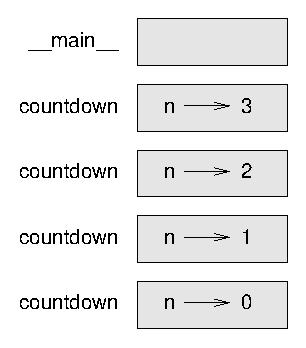
\includegraphics{figs/stack2.eps}}
%\afterfig

%\index{base case}
%\index{recursion!base case}

%The four {\tt countdown} frames have different values for the
%parameter {\tt n}.  The bottom of the stack, where {\tt n=0}, is
%called the {\bf base case}.  It does not make a recursive call, so
%there are no more frames.

%\begin{ex}
%Draw a stack diagram for \verb"print_n" called with
%\verb"s = 'Hello'" and {\tt n=2}.
%\end{ex}

\section{Infinite recursion}
\index{infinite recursion}
\index{recursion!infinite}
\index{runtime error}
\index{error!runtime}
\index{traceback}

If a recursion never reaches a base case, it goes on making
recursive calls forever, and the program never terminates.  This is
known as {\bf infinite recursion}, and it is generally not
a good idea.  The most common source of infinite recursion
is forgetting to decrement when you make the recursive call:

\beforeverb
\begin{verbatim}
let rec csum n = 
	if n = 0
	then 0
	else (n + csum n);;\end{verbatim}
\afterverb
%
In most programming environments, a program with infinite recursion
does not really run forever. Usually, you run out of what they call
``stack space'', which is a function of your computer architecture.

\index{exception!RuntimeError}
\index{RuntimeError}

\beforeverb
\begin{verbatim}
# csum 10;;
Stack overflow during evaluation (looping recursion?).
\end{verbatim}
\afterverb

The error can also occur if the program doesn't reach the base case
for any reason. {\tt csum}, for example, isn't particularly robust:
if we give it a negative number, it explodes.

\beforeverb
\begin{verbatim}
# csum (-2);;
Stack overflow during evaluation (looping recursion?).
\end{verbatim}
\afterverb

{\tt csum} will continue subtracting from $-2$ ad infinitum without 
ever reaching 0, so it will keep going until it runs out of space.
This could be easily avoided by checking to make sure the argument 
is non-negative.

\section{Mutually Recursive Functions}

It's not really that common, but every once in a while you might want
to define recursive functions that call each other. Here's a trivial 
example:\footnote{Thanks to Ryan Tarpine who submitted it to 
ocaml-tutorial.org} 0 is an even number, and a number is defined as 
even if its predecessor is odd. Naturally, we could easily just check
{\tt x mod 2} to see if x is even, but that wouldn't be pedagogically
as interesting as this:

\beforeverb
\begin{verbatim}
let rec even x = 
	if x = 0
	then true
	else odd (x-1);;
let rec odd x = 
	if x = 0
	then false
	else even (x-1);;
\end{verbatim}
\afterverb

Not the prettiest solution, but it should work, right? Well, actually, no.
Because of how OCaml compiles, it would need odd first to compile even, but
would also need even first to compile odd. Somehow we need to tell OCaml to
compile both functions at the same time. Fortunately, OCaml comes with a 
syntax to do this:

\beforeverb
\begin{verbatim}
let rec even x = 
	if x = 0
	then true
	else odd (x-1)
and odd x = 
	if x = 0
	then false
	else even (x-1);;
\end{verbatim}
\afterverb

\section{Tail-end Recursion}

\index{Tail-end Recursion}
\index{Recursion!Tail-end}

Remember {\tt csum}? Well, it looked like this:

\beforeverb
\begin{verbatim}
let rec csum n = 
	if n=1
	then 1
	else n + (csum (n-1));;
\end{verbatim}
\afterverb

This is a perfectly valid, and reasonably efficient solution to this
problem, and the code is very easy to follow. However, there's one 
problem with this code: as n increases, we make proportionally more 
function calls to csum, each of which takes up a little bit of memory.
For most situations, this is probably fine, and certainly in this case,
we'd have to give it a relatively huge integer for most modern computers 
to run out of memory. However, for other programs, we might want to be 
able to write recursive functions that don't build up on that stack. But 
how can we do that?

The answer is called {\bf tail-end recursion}. The general idea is to write
your recursive function such that the value returned by the recursive call 
is what's returned by your function, i.e., there's no pending operation 
in the function waiting for the value returned by the recursive call. That 
way, the function can say, "Don't bother with me anymore, just take the answer 
from my recursive call as the result. You can just forget all of my state 
information."

Generally, in order to implement tail-end recursion we need an extra argument 
that accumulates the result along the way, so the inner-most recursive call
has all the information from the steps before it. Going back to our summing 
example, you might implement it like this:

\beforeverb
\begin{verbatim}
let rec csum_helper accum n = 
	if n=1
	then (accum+1)
	else (csum_helper (accum+n)) (n-1);;

let csum = csum_helper 0;;
\end{verbatim}
\afterverb.

Note how {\tt \verb"csum_helper"}'s return value is either the answer or simply the 
result of the recursive call. Hence, the computer does not need to keep this 
function around, it just needs to take the value from the recursive call. Also, 
note how I've arranged this program: because I needed an {\tt accum} argument, 
but when I call the function that will always be {\tt 0}, I've seperated this 
into two functions, a {\bf helper function} and a {\bf call function}. All the 
work happens in the helper function, but I don't want to have to tell it that
{\tt accum} is (in the first call) just zero every time I want to call the 
function, so I write another function to do that for me (which I defined using
currying!).

Tail-recursion is generally faster and requires less memory than standard recursion. 
However, it can be hard to see a tail-recursive solution the first time writing an 
algorithm, so it's often easier to write a standard recursion solution and then figure 
out a tail-recursive algorithm based on that code. Also, tail-recursive solutions are 
usually much less clear than standard recursion, so in cases where other people will be 
reading your code and you don't need to worry about the memory used, it's often better 
to just use standard recursion. Finally, there might not always be an obvious tail-recursive
solution and it might not be the best use of your time to find an algorithm if it won't 
significantly improve your code's performance.

Now, you may be wondering how computers know that this function is tail-recursive.
The answer is, they don't, but some compilers do. OCaml implements tail-recursion 
as a standard of the language, as do many other functional programming languages. 
However, many other programming languages, such as Python, do not implement 
tail-recursion. If you learn other programming languages later, make sure to find 
out whether or not they implement tail-recursion before using it, or else you'll 
gain nothing but harder-to-read code.

\section{Debugging}
\label{whitespace}
\index{debugging}
\index{traceback}
%edit here!
The traceback OCaml displays when an error occurs contains
a lot of information, but it can be overwhelming, especially
when there are many frames on the stack.  The most
useful parts are usually:

\begin{itemize}

\item What kind of error it was, and

\item Where it occurred.

\end{itemize}

In general, error messages indicate where the problem was
discovered, but the actual error might be earlier in the code,
sometimes on a previous line.

\section{Glossary}

\begin{description}

\item[recursion:]  The process of calling the function that is
currently executing.
\index{recursion}

\item[base case:]  A conditional branch in a
recursive function that does not make a recursive call.
\index{base case}

\item[infinite recursion:]  A recursive function that doesn't have a
base case, or never reaches it.  Eventually, an infinite recursion
causes a runtime error.
\index{infinite recursion}

\item[tail-end recursion:] A recursive function whose result is either 
the base case or the result of a recursive call, and hence does not have
an operation pending for the result of said recursive call.
\index{tail-end recursion}

\end{description}

\section{Exercises}

\begin{ex}
You've probably heard of the fibonacci numbers before, but in case you haven't, they're defined by the following recursive relationship: \footnote{Sometimes the specifics of the base cases looks a little different, but it all works out to be the same series.}

\begin{eqnarray*}
f(0) &=& 0 \\
f(1) &=& 1 \\
f(n+1) &=& f(n) + f(n-1)
\end{eqnarray*}

Write a recursive function to calculate these numbers. It does not need to be tail recursive.

\end{ex} \label{ex:fibonacci}

\begin{ex}
\index{Ackerman function}
\index{function!ack}

The Ackermann function, $A(m, n)$, is defined\footnote{See
  \url{wikipedia.org/wiki/Sometimes the specifics of the base cases looks a little different, but it all works out to be the same series.Ackermann_function}.}:

\begin{eqnarray}
A(m, n) = \begin{cases} 
              n+1 & \mbox{if } m = 0 \\ 
        A(m-1, 1) & \mbox{if } m > 0 \mbox{ and } n = 0 \\ 
A(m-1, A(m, n-1)) & \mbox{if } m > 0 \mbox{ and } n > 0.
\end{cases} 
\end{eqnarray}
%
Write a function named {\tt ack} that evaluates Ackerman's function.
Use your function to evaluate {\tt ack(3, 4)}, which should be 125.
What happens for larger values of {\tt m} and {\tt n}?

\end{ex}


\begin{ex}
\label{palindrome}

\index{palindrome}

A palindrome is a word that is spelled the same backward and
forward, like ``noon'' and ``redivider''.  Recursively, a word
is a palindrome if the first and last letters are the same
and the middle is a palindrome.

The following are functions that take a string argument and
return the first, last, and middle letters:

\beforeverb
\begin{verbatim}
let first_char word = word.[0];;

let last_char word =
	let len = String.length word - 1
	in word.[len];;

let middle word = 
	let len = String.length word - 2 in
	String.sub word 1 len;;
\end{verbatim}
\afterverb
%edit here
Note that these function use syntax you haven't seen yet. 
We'll see how they work in Chapter~\ref{strings}.

\begin{enumerate}

\item Type these functions into a file named {\tt palindrome.ml}
and test them out.  What happens if you call {\tt middle} with
a string with two letters?  One letter?  What about the empty
string, which is written \verb"''" and contains no letters?

\item Write a function called \verb"is_palindrome" that takes
a string argument and returns {\tt True} if it is a palindrome
and {\tt False} otherwise.  Remember that you can use the
built-in function {\tt len} to check the length of a string.

\end{enumerate}

\end{ex}

\begin{ex}
A number, $a$, is a power of $b$ if it is divisible by $b$
and $a/b$ is a power of $b$.  Write a function called
\verb"is_power" that takes parameters {\tt a} and {\tt b}
and returns {\tt True} if {\tt a} is a power of {\tt b}.
\end{ex}


\begin{ex}

\index{greatest common divisor (GCD)}
\index{GCD (greatest common divisor)}

The greatest common divisor (GCD) of $a$ and $b$ is the largest number
that divides both of them with no remainder\footnote{This exercise is
  based on an example from Abelson and Sussman's {\em Structure and
    Interpretation of Computer Programs}.}.

One way to find the GCD of two numbers is Euclid's algorithm,
which is based on the observation that if $r$ is the remainder
when $a$ is divided by $b$, then $gcd(a, b) = gcd(b, r)$.
As a base case, we can consider $gcd(a, 0) = a$.

\index{Euclid's algorithm}
\index{algorithm!Euclid}

Write a function called
\verb"gcd" that takes parameters {\tt a} and {\tt b}
and returns their greatest common divisor.  If you need
help, see \url{wikipedia.org/wiki/Euclidean_algorithm}.

\end{ex}

\begin{ex}

The Hofstadter Female and Male sequences are two sequences of integers
defined in terms of each other, such that:

\begin{align*}
F(0) &= 1; M(0) = 0 \\
F(n) &= n - M(F(n-1)), n>0 \\
M(n) &= n - F(M(n-1)), n>0
\end{align*}

The first few terms of the sequences are:

\begin{align*}
F:& 1, 1, 2, 2, 3, 3, 4, 5, 5,... \\
M:& 0, 0, 1, 2, 2, 3, 4, 4, 5,... 
\end{align*}

Write two mutually recursive functions to find the n-th term of the 
sequences.

\end{ex}

\chapter{Algorithms}
%serious edit here!!

\section{Square roots}

\index{square root}

Recursion or looping is often used in programs that compute
numerical results by starting with an approximate answer and
iteratively improving it.

\index{Newton's method}

For example, one way of computing square roots is Newton's method.
Suppose that you want to know the square root of $a$.  If you start
with almost any estimate, $x$, you can compute a better
estimate with the following formula:

\[ y = \frac{x + a/x}{2} \]
%
For example, if $a$ is 4 and $x$ is 3:

\beforeverb
\begin{verbatim}
# let a = 4.0;;
# let x = 3.0;;
# let y = (x +. a/.x) /. 2.0;;
val y : float = 2.16666666666666652
\end{verbatim}
\afterverb
%
Which is closer to the correct answer ($\sqrt{4} = 2$).  If we
repeat the process with the new estimate, it gets even closer:

\beforeverb
\begin{verbatim}
# let x = y;;
# let y = (x +. a/.x) /. 2.0;;
val y : float = 2.00641025641025639
\end{verbatim}
\afterverb
%
After a few more updates, the estimate is almost exact:

\beforeverb
\begin{verbatim}
# let x = y;;
# let y = (x +. a/.x) /. 2;;
val y : float = 2.00001024002621453
# let x = y;;
# let y = (x +. a/.x) /. 2;;
val y : float = 2.00000000002621459
\end{verbatim}
\afterverb
%
In general we don't know ahead of time how many steps it takes
to get to the right answer, but we know when we get there
because the estimate
stops changing:

\beforeverb
\begin{verbatim}
# let x = 2.0;;
# let y = (x +. a/.x) /. 2;;
val y : float = 2.
# let x = y;;
# let y = (x +. a/.x) /. 2;;
val y : float = 2.
\end{verbatim}
\afterverb
%
When {\tt y == x}, we can stop.  Here is a function that starts
with an initial estimate, {\tt x}, and improves it until it
stops changing:

\beforeverb
\begin{verbatim}
let rec sqroot a x y = 
	if x=y
	then y
	else let ynew = (x +. a/.x) /. 2.0
		in sqroot a y ynew;;
\end{verbatim}
\afterverb
%
For most values of {\tt a} this works fine, but in general it is
dangerous to test {\tt float} equality.
Floating-point values are only approximately right:
most rational numbers, like $1/3$, and irrational numbers, like
$\sqrt{2}$, can't be represented exactly with a {\tt float}.

\index{floating-point}
\index{epsilon}

Rather than checking whether {\tt x} and {\tt y} are exactly equal, it
is safer to use the built-in function {\tt abs} to compute the
absolute value, or magnitude, of the difference between them:

\beforeverb
\begin{verbatim}
    if abs (y-x) < epsilon
\end{verbatim}
\afterverb
where \verb"epsilon" has a value like {\tt 0.0000001} that
determines how close is close enough.

\begin{ex}
\label{square_root}
\index{encapsulation}

Encapsulate this recursive function called \verb"square_root"
that takes {\tt a} as a parameter, chooses a reasonable
value of {\tt x}, and returns an estimate of the square root
of {\tt a}.
\end{ex}

\section{Algorithms}
\index{algorithm}

Newton's method is an example of an {\bf algorithm}: it is a
mechanical process for solving a category of problems (in this
case, computing square roots).

It is not easy to define an algorithm.  It might help to start
with something that is not an algorithm.  When you learned
to multiply single-digit numbers, you probably memorized the
multiplication table.  In effect, you memorized 100 specific solutions.
That kind of knowledge is not algorithmic.

But if you were ``lazy,'' you probably cheated by learning a few
tricks.  For example, to find the product of $n$ and 9, you can
write $n-1$ as the first digit and $10-n$ as the second
digit.  This trick is a general solution for multiplying any
single-digit number by 9.  That's an algorithm!

\index{addition with carrying}
\index{carrying, addition with}
\index{subtraction!with borrowing}
\index{borrowing, subtraction with}

Similarly, the techniques you learned for addition with carrying,
subtraction with borrowing, and long division are all algorithms.  One
of the characteristics of algorithms is that they do not require any
intelligence to carry out.  They are mechanical processes in which
each step follows from the last according to a simple set of rules.

In my opinion, it is embarrassing that humans spend so much time in
school learning to execute algorithms that, quite literally, require
no intelligence.

On the other hand, the process of designing algorithms is interesting,
intellectually challenging, and a central part of what we call
programming.

Some of the things that people do naturally, without difficulty or
conscious thought, are the hardest to express algorithmically.
Understanding natural language is a good example.  We all do it, but
so far no one has been able to explain {\em how} we do it, at least
not in the form of an algorithm.


\section{Debugging}

As you start writing bigger programs, you might find yourself
spending more time debugging.  More code means more chances to
make an error and more place for bugs to hide.

\index{debugging!by bisection}
\index{bisection, debugging by}

One way to cut your debugging time is ``debugging by bisection.''
For example, if there are 100 lines in your program and you
check them one at a time, it would take 100 steps.

Instead, try to break the problem in half.  Look at the middle
of the program, or near it, for an intermediate value you
can check.  Add a {\tt print} statement (or something else
that has a verifiable effect) and run the program.

If the mid-point check is incorrect, there must be a problem in the
first half of the program.  If it is correct, the problem is
in the second half.

Every time you perform a check like this, you halve the number of
lines you have to search.  After six steps (which is fewer than 100),
you would be down to one or two lines of code, at least in theory.

In practice it is not always clear what
the ``middle of the program'' is and not always possible to
check it.  It doesn't make sense to count lines and find the
exact midpoint.  Instead, think about places
in the program where there might be errors and places where it
is easy to put a check.  Then choose a spot where you
think the chances are about the same that the bug is before
or after the check.

\section{Glossary}

\begin{description}
%write things here!
\item stuff

\end{description}


\section{Exercises}

\begin{ex}

\index{algorithm!square root}

To test the square root algorithm in this chapter, you could compare
it with {\tt sqrt}.  Write a function named \verb"test_square_root"
that prints a table something like this:

\beforeverb
\begin{verbatim}
1.0 1.0           1.0           0.0
2.0 1.41421356237 1.41421356237 2.22044604925e-16
3.0 1.73205080757 1.73205080757 0.0
4.0 2.0           2.0           0.0
5.0 2.2360679775  2.2360679775  0.0
6.0 2.44948974278 2.44948974278 0.0
7.0 2.64575131106 2.64575131106 0.0
8.0 2.82842712475 2.82842712475 4.4408920985e-16
9.0 3.0           3.0           0.0

\end{verbatim}
\afterverb
%
The first column is a number, $a$; the second column is
the square root of $a$ computed with the function from
Exercise~\ref{square_root}; the third column is the square root computed
by {\tt sqrt}; the fourth column is the absolute value
of the difference between the two estimates.
\end{ex}

\begin{ex}

\index{Ramanujan, Srinivasa}

The brilliant mathematician Srinivasa Ramanujan found an
infinite series\footnote{See \url{wikipedia.org/wiki/Pi}.}
that can be used to generate a numerical
approximation of $\pi$:

\index{pi}

\[\frac{1}{\pi} = \frac{2\sqrt{2}}{9801} 
\sum^\infty_{k=0} \frac{(4k)!(1103+26390k)}{(k!)^4 396^{4k}} \]

Write a function called \verb"estimate_pi" that uses this formula
to compute and return an estimate of $\pi$.  It should use recursion 
to compute terms of the summation until the last term is
smaller than {\tt 10.**(-15)}.
\end{ex}


\chapter{Strings}
\label{strings}


\section{A string is a sequence}
\index{sequence}
\index{character}
\index{bracket operator}
\index{operator!bracket}

A string is a {\bf sequence} of characters.  
You can access the characters one at a time with the
bracket operator:

\beforeverb
\begin{verbatim}
# let fruit = "banana";;
# let letter = fruit.[1]
\end{verbatim}
\afterverb
%
The second statement selects character number 1 from {\tt
fruit} and assigns it to {\tt letter}. Note that the type 
of {\tt letter} is {\tt char} not {\tt string}.

\index{index}

The expression in brackets is called an {\bf index}.  
The index indicates which character in the sequence you
want (hence the name).

But you might not get what you expect:

\beforeverb
\begin{verbatim}
# letter
- : char = 'a'
\end{verbatim}
\afterverb
%
For most people, the first letter of \verb"'banana'" is {\tt b}, not
{\tt a}.  But for computer scientists, the index is an offset from the
beginning of the string, and the offset of the first letter is zero.

\beforeverb
\begin{verbatim}
let letter = fruit.[0]
val letter : char = 'b'
\end{verbatim}
\afterverb
%
So {\tt b} is the 0th letter (``zero-eth'') of \verb"'banana'", {\tt a}
is the 1th letter (``one-eth''), and {\tt n} is the 2th (``two-eth'')
letter.

\index{index!starting at zero}
\index{zero, index starting at}

You can use any expression, including variables and operators, as an
index, but the value of the index has to be an integer.  Otherwise you
get:

\index{index}
\index{exception!TypeError}
\index{TypeError}

\beforeverb
\begin{verbatim}
# let letter = fruit[1.5]
Error: This expression has type float but an expression was expected of type
	 int.
\end{verbatim}
\afterverb
%

Note that {\tt fruit.[i]} is the same as typing {\tt String.get fruit i}.

Strings are mutable; you can change the value of characters within the 
string using the {\tt set} function:

\beforeverb
\begin{verbatim}
# fruit.[1]<-'b';;
- : unit = ()
# fruit;;
- : string = "bbnana"
\end{verbatim}
\afterverb

Note that this is equivalent to writing {\tt String.set fruit 1 'b'}. If you 
try to set a character outside of a string, then you'll get an exception error.

\section{{\tt String.length}}

\index{String module}
\index{String.length function}
\index{function!String.length}

Many useful string operations can be found in the {\tt String} module.
{\tt String.length} is a built-in function that returns the number of 
characters in a string:

\beforeverb
\begin{verbatim}
>>> fruit = 'banana'
>>> len(fruit)
6
\end{verbatim}
\afterverb
%
To get the last letter of a string, you might be tempted to try something
like this:

\index{exception!IndexError}
\index{IndexError}

\beforeverb
\begin{verbatim}
# let len = String.legnth fruit;;
# let last = fruit.[length];;
Exception: Invalid_argument "index out of bounds"
\end{verbatim}
\afterverb
%
The reason for the {\tt Exception} is that there is no letter in {\tt
'banana'} with the index 6.  Since we started counting at zero, the
six letters are numbered 0 to 5.  To get the last character, you have
to subtract 1 from {\tt length}:

\beforeverb
\begin{verbatim}
# let last = fruit[len-1]
val last: char = 'a'
\end{verbatim}
\afterverb
%

\section{Substrings}

One thing you'll want to be able to do with strings is select {\bf substrings},
or sections of strings that are themselves strings. We saw an example of this 
before in the palindromes exercise:

\beforeverb
\begin{verbatim}
let middle word = 
	let len = String.length word - 2 in
	String.sub word 1 len
\end{verbatim}
\afterverb
In this example, we're extracting the substring of all the characters between 
the first and last character.


\section{String Traversal}
\label{for}

\index{traversal}
\index{recursion!traversal}

A lot of computations involve processing a string one character at a
time.  Often they start at the beginning, select each character in
turn, do something to it, and continue until the end.  This pattern of
processing is called a {\bf traversal}.  One way to write a traversal
is with recursion and substrings:

\beforeverb
\begin{verbatim}
let rec traverse_print s = 
	print_char s.[0]; print_newline();
	let len = String.length s in
		if len=1
		then ()
		else traverse_print (String.sub s 1 (len - 1));;\end{verbatim}
\afterverb
%
This function traverses the string and displays each letter on a line by
itself. It does this by using a recursive loop that prints the first letter
than recursively calls itself on the substring that is the string without
the first letter.

\begin{ex}
Write a function that takes a string as an argument
and displays the letters backward, one per line.
\end{ex}

\index{concatenation}
\index{abecedarian}
\index{McCloskey, Robert}

The following example shows how to use concatenation (string addition)
and a {\tt for} loop to generate an abecedarian series (that is, in
alphabetical order).  In Robert McCloskey's book {\em Make
Way for Ducklings}, the names of the ducklings are Jack, Kack, Lack,
Mack, Nack, Ouack, Pack, and Quack.  This loop outputs these names in
order:

\beforeverb
\begin{verbatim}
let prefixes = "JKLMNOPQ";;
let suffix = "ack";;

let rec ducklings prefixes suffix = 
	let prefix = String.sub prefixes 0 1 in
	print_string (prefix^suffix); print_newline();
	let len = String.length prefixes in
		if len == 1
		then ()
		else ducklings (String.sub prefixes 1 (len-1)) suffix;;
\end{verbatim}
\afterverb
%
The output is:

\beforeverb
\begin{verbatim}
Jack
Kack
Lack
Mack
Nack
Oack
Pack
Qack
- : unit = ()
\end{verbatim}
\afterverb
%
Of course, that's not quite right because ``Ouack'' and
``Quack'' are misspelled.

\begin{ex}
Modify the program to fix this error.
\end{ex}

\section{Searching}
\label{find}

What does the following code do?

\index{find function}
\index{function!find}

\beforeverb
\begin{verbatim}
let rec find_helper ctr word letter = 
	if word.[0]=letter
	then ctr
	else let len = String.length word in
		if len = 1
		then -1
		else
		let ctr = ctr+1 in
		let word = String.sub word 1 (len-1) in
		find_helper ctr word letter;;

let find = find_helper 0;;
\end{verbatim}
\afterverb
%
In a sense, {\tt find} is the opposite of the {\tt .[]} operator.
Instead of taking an index and extracting the corresponding character,
it takes a character and finds the index where that character
appears.  If the character is not found, the function returns {\tt
-1}.

If the character doesn't appear in the string, the function returns 
{\tt -1}.

This pattern of computation---traversing a sequence and returning
when we find what we are looking for---is a called a {\bf search}.

\index{traversal}
\index{search pattern}
\index{pattern!search}

\begin{ex}
Modify {\tt find} so that it finds the last
instance of the letter, rather than the first.
\end{ex}

\begin{ex}
Modify {\tt find} so that it has a
third parameter, the index in {\tt word} where it should start
looking.
\end{ex}

\begin{ex}
Write a function {\tt count} that takes a string input and a 
character input and counts the number of times that character
appears and returns that value.
\end{ex}

\section{String comparison}

\index{string!comparison}
\index{comparison!string}

The relational operators work on strings.  To see if two strings are equal:

\beforeverb
\begin{verbatim}
if word = "banana":
    then print_string  "All right, bananas. \n";;
\end{verbatim}
\afterverb
%
Other relational operations are useful for putting words in alphabetical
order:

\beforeverb
\begin{verbatim}
let is_bananas word = print_string
	(match word with 
	"bananas" -> "Your string is bananas! \n"
	| w when w<"bananas" -> word^" is less than bananas. \n"
	| _ -> word^" is more than bananas. \n");;
\end{verbatim}
\afterverb

OCaml does not handle uppercase and lowercase letters the same way
that people do.  All the uppercase letters come before all the
lowercase letters, so:

\beforeverb
\begin{verbatim}
# is_bananas "pineapple";;
pineapple is more than bananas.
- : unit = ()
# is_bananas "Pineapple";;
Pineapple is less than bananas.
- : unit = ()
\end{verbatim}
\afterverb
%
A common way to address this problem is to convert strings to a
standard format, such as all lowercase, before performing the
comparison.  Keep that in mind in case you have to defend yourself
against a man armed with a Pineapple.

\section{Debugging}
\index{debugging}

\index{traversal}

When you use indices to traverse the values in a sequence,
it is tricky to get the beginning and end of the traversal
right. For debugging this kind of error, first try printing
the values of the indices immediately before the line where 
the error appears. Now when you run the program again, you'll 
get more information:

%edit here - provide example (Allen's was to check if two strings are the reverse of each other.)

\section{Glossary}

\begin{description}
%edit here
\item[sequence:] An ordered set; that is, a set of
values where each value is identified by an integer index.
\index{sequence}

\item[item:] One of the values in a sequence.
\index{item}

\item[index:] An integer value used to select an item in
a sequence, such as a character in a string.
\index{index}

\item[slice:] A part of a string specified by a range of indices.
\index{slice}

\item[empty string:] A string with no characters and length 0, represented
by two quotation marks.
\index{empty string}

\item[immutable:] The property of a sequence whose items cannot
be assigned.
\index{immutability}

\item[traverse:] To iterate through the items in a sequence,
performing a similar operation on each.
\index{traversal}

\item[search:] A pattern of traversal that stops
when it finds what it is looking for.
\index{search pattern}
\index{pattern!search}

\item[counter:] A variable used to count something, usually initialized
to zero and then incremented.
\index{counter}

\item[method:] A function that is associated with an object and called
using dot notation.
\index{method}

\item[invocation:] A statement that calls a method.
\index{invocation}

\end{description}


\section{Exercises}

\begin{ex}
\index{string method}
\index{method!string}

Read the documentation of the String module at
\url{http://caml.inria.fr/pub/docs/manual-ocaml/libref/String.html}.
You might want to experiment with some of them to make sure
you understand how they work.  {\tt index} and
{\tt iter} are particularly useful.

\end{ex}

% \begin{ex}
% The following functions are all {\em intended} to check whether a
% string contains any lowercase letters, but at least some of them are
% wrong.  For each function, describe what the function actually does
% (assuming that the parameter is a string).
% %edit here
% \beforeverb
% \begin{verbatim}
% def any_lowercase1(s):
%     for c in s:
%         if c.islower():
%             return True
%         else:
%             return False
% 
% def any_lowercase2(s):
%     for c in s:
%         if 'c'.islower():
%             return 'True'
%         else:
%             return 'False'
% 
% def any_lowercase3(s):
%     for c in s:
%         flag = c.islower()
%     return flag
% 
% def any_lowercase4(s):
%     flag = False
%     for c in s:
%         flag = flag or c.islower()
%     return flag
% 
% def any_lowercase5(s):
%     for c in s:
%         if not c.islower():
%             return False
%     return True
% \end{verbatim}
% \afterverb
% 
% \end{ex}
% 

\begin{ex}
\index{letter rotation}
\index{rotation, letter}

\label{exrotate}
ROT13 is a weak form of encryption that involves ``rotating'' each
letter in a word by 13 places\footnote{See
  \url{wikipedia.org/wiki/ROT13}.}.  To rotate a letter means
to shift it through the alphabet, wrapping around to the beginning if
necessary, so 'A' shifted by 3 is 'D' and 'Z' shifted by 1 is 'A'.

Write a function called \verb"rotate_word"
that takes a string and an integer as parameters, and that returns
a new string that contains the letters from the original string
``rotated'' by the given amount.  

For example, ``cheer'' rotated by 7 is ``jolly'' and ``melon'' rotated
by -10 is ``cubed''.  

%For example ``sleep''
%rotated by 9 is ``bunny'' and ``latex'' rotated by 7 is ``shale''.

You might want to use the built-in {\tt String.iter} function, and
you'll probably find at least a couple of the functions at
\url{http://gallium.inria.fr/~remy/poly/ocaml/htmlman/libref/Char.html}
useful.

Potentially offensive jokes on the Internet are sometimes encoded
in ROT13.  If you are rather bored by not easily offended, find and 
decode some of them.
\end{ex}


% \chapter{Case study: word play}
% 
% \section{Reading word lists}
% \label{wordlist}
% 
% For the exercises in this chapter we need a list of English words.
% There are lots of word lists available on the Web, but the one most
% suitable for our purpose is one of the word lists collected and
% contributed to the public domain by Grady Ward as part of the Moby
% lexicon project\footnote{\url{wikipedia.org/wiki/Moby_Project}.}.  It
% is a list of 113,809 official crosswords; that is, words that are
% considered valid in crossword puzzles and other word games.  In the
% Moby collection, the filename is {\tt 113809of.fic}; I include a copy
% of this file, with the simpler name {\tt words.txt}, along with
% Swampy.
% 
% \index{Swampy}
% \index{crosswords}
% 
% This file is in plain text, so you can open it with a text
% editor, but you can also read it from Python.  The built-in
% function {\tt open} takes the name of the file as a parameter
% and returns a {\bf file object} you can use to read the file.
% 
% \index{open function}
% \index{function!open}
% \index{plain text}
% \index{text!plain}
% \index{object!file}
% \index{file object}
% 
% \beforeverb
% \begin{verbatim}
% >>> fin = open('words.txt')
% >>> print fin
% <open file 'words.txt', mode 'r' at 0xb7f4b380>
% \end{verbatim}
% \afterverb
% %
% {\tt fin} is a common name for a file object used for
% input.  Mode \verb"'r'" indicates that this file is open for
% reading (as opposed to \verb"'w'" for writing).
% 
% \index{readline method}
% \index{method!readline}
% 
% The file object provides several methods for reading, including
% {\tt readline}, which reads characters from the file
% until it gets to a newline and returns the result as a
% string:
% 
% \beforeverb
% \begin{verbatim}
% >>> fin.readline()
% 'aa\r\n'
% \end{verbatim}
% \afterverb
% %
% The first word in this particular list is ``aa,'' which is a kind of
% lava.  The sequence \verb"\r\n" represents two whitespace characters,
% a carriage return and a newline, that separate this word from the
% next.
% 
% The file object keeps track of where it is in the file, so
% if you call {\tt readline} again, you get the next word:
% 
% \beforeverb
% \begin{verbatim}
% >>> fin.readline()
% 'aah\r\n'
% \end{verbatim}
% \afterverb
% %
% The next word is ``aah,'' which is a perfectly legitimate
% word, so stop looking at me like that.
% Or, if it's the whitespace that's bothering you,
% we can get rid of it with the string method {\tt strip}:
% 
% \index{strip method}
% \index{method!strip}
% 
% \beforeverb
% \begin{verbatim}
% >>> line = fin.readline()
% >>> word = line.strip()
% >>> print word
% aahed
% \end{verbatim}
% \afterverb
% %
% You can also use a file object as part of a {\tt for} loop.
% This program reads {\tt words.txt} and prints each word, one
% per line:
% 
% \index{open function}
% \index{function!open}
% 
% \beforeverb
% \begin{verbatim}
% fin = open('words.txt')
% for line in fin:
%     word = line.strip()
%     print word
% \end{verbatim}
% \afterverb
% %
% 
% \begin{ex}
% Write a program that reads {\tt words.txt} and prints only the
% words with more than 20 characters (not counting whitespace).
% 
% \index{whitespace}
% 
% \end{ex}
% 
% \section{Exercises}
% 
% There are solutions to these exercises in the next section.
% You should at least attempt each one before you read the solutions.
% 
% \begin{ex}
% In 1939 Ernest Vincent Wright published a 50,000 word novel called
% {\em Gadsby} that does not contain the letter ``e.''  Since ``e'' is
% the most common letter in English, that's not easy to do.
% 
% In fact, it is difficult to construct a solitary thought without using
% that most common symbol.  It is slow going at first, but with caution
% and hours of training you can gradually gain facility.
% 
% All right, I'll stop now.
% 
% Write a function called \verb"has_no_e" that returns {\tt True} if
% the given word doesn't have the letter ``e'' in it.
% 
% Modify your program from the previous section to print only the words
% that have no ``e'' and compute the percentage of the words in the list
% have no ``e.''
% 
% \index{lipogram}
% 
% \end{ex}
% 
% 
% \begin{ex} 
% Write a function named {\tt avoids}
% that takes a word and a string of forbidden letters, and
% that returns {\tt True} if the word doesn't use any of the forbidden
% letters.
% 
% Modify your program to prompt the user to enter a string
% of forbidden letters and then print the number of words that
% don't contain any of them.
% Can you find a combination of 5 forbidden letters that
% excludes the smallest number of words?
% \end{ex}
% 
% \begin{ex}
% Write a function named \verb"uses_only" that takes a word and a
% string of letters, and that returns {\tt True} if the word contains
% only letters in the list.  Can you make a sentence using only the
% letters {\tt acefhlo}?  Other than ``Hoe alfalfa?''
% \end{ex}
% 
% \begin{ex} 
% Write a function named \verb"uses_all" that takes a word and a
% string of required letters, and that returns {\tt True} if the word
% uses all the required letters at least once.  How many words are there
% that use all the vowels {\tt aeiou}?  How about {\tt aeiouy}?
% \end{ex}
% 
% \begin{ex}
% Write a function called \verb"is_abecedarian" that returns
% {\tt True} if the letters in a word appear in alphabetical order
% (double letters are ok).  
% How many abecedarian words are there?
% \end{ex}
% 
% \index{abecedarian}
% 
% 
% %\begin{ex}
% %\label{palindrome}
% %A palindrome is a word that reads the same
% %forward and backward, like ``rotator'' and ``noon.''
% %Write a boolean function named \verb"is_palindrome" that
% %takes a string as a parameter and returns {\tt True} if it is
% %a palindrome.
% 
% %Modify your program from the previous section to print all
% %of the palindromes in the word list and then print the total
% %number of palindromes.
% %\end{ex}
% 
% 
% 
% \section{Search}
% 
% \index{search pattern}
% \index{pattern!search}
% 
% All of the exercises in the previous section have something
% in common; they can be solved with the search pattern we saw
% in Section~\ref{find}.  The simplest example is:
% 
% \beforeverb
% \begin{verbatim}
% def has_no_e(word):
%     for letter in word:
%         if letter == 'e':
%             return False
%     return True
% \end{verbatim}
% \afterverb
% %
% The {\tt for} loop traverses the characters in {\tt word}.  If we find
% the letter ``e'', we can immediately return {\tt False}; otherwise we
% have to go to the next letter.  If we exit the loop normally, that
% means we didn't find an ``e'', so we return {\tt True}.
% 
% \index{traversal}
% 
% % Removing this because we haven't seen the in operator yet.
% %\index{in operator}
% %\index{operator!in}
% 
% %You could write this function more concisely using the {\tt in}
% %operator, but I started with this version because it 
% %demonstrates the logic of the search pattern.
% 
% \index{generalization}
% 
% {\tt avoids} is a more general version of \verb"has_no_e" but it
% has the same structure:
% 
% \beforeverb
% \begin{verbatim}
% def avoids(word, forbidden):
%     for letter in word:
%         if letter in forbidden:
%             return False
%     return True
% \end{verbatim}
% \afterverb
% %
% We can return {\tt False} as soon as we find a forbidden letter;
% if we get to the end of the loop, we return {\tt True}.
% 
% \verb"uses_only" is similar except that the sense of the condition
% is reversed:
% 
% \beforeverb
% \begin{verbatim}
% def uses_only(word, available):
%     for letter in word: 
%         if letter not in available:
%             return False
%     return True
% \end{verbatim}
% \afterverb
% %
% Instead of a list of forbidden letters, we have a list of available
% letters.  If we find a letter in {\tt word} that is not in
% {\tt available}, we can return {\tt False}.
% 
% \verb"uses_all" is similar except that we reverse the role
% of the word and the string of letters:
% 
% \beforeverb
% \begin{verbatim}
% def uses_all(word, required):
%     for letter in required: 
%         if letter not in word:
%             return False
%     return True
% \end{verbatim}
% \afterverb
% %
% Instead of traversing the letters in {\tt word}, the loop
% traverses the required letters.  If any of the required letters
% do not appear in the word, we can return {\tt False}.
% 
% \index{traversal}
% 
% If you were really thinking like a computer scientist, you would
% have recognized that \verb"uses_all" was an instance of a
% previously-solved problem, and you would have written:
% 
% \beforeverb
% \begin{verbatim}
% def uses_all(word, required):
%     return uses_only(required, word)
% \end{verbatim}
% \afterverb
% %
% This is an example of a program development method called {\bf problem
% recognition}, which means that you recognize the problem you are
% working on as an instance of a previously-solved problem, and apply a
% previously-developed solution.
% 
% \index{problem recognition}
% \index{development plan!problem recognition}
% 
% 
% \section{Looping with indices}
% 
% \index{looping!with indices}
% \index{index!looping with}
% 
% I wrote the functions in the previous section with {\tt for}
% loops because I only needed the characters in the strings; I didn't
% have to do anything with the indices.
% 
% For \verb"is_abecedarian" we have to compare adjacent letters,
% which is a little tricky with a {\tt for} loop:
% 
% \beforeverb
% \begin{verbatim}
% def is_abecedarian(word):
%     previous = word[0]
%     for c in word:
%         if c < previous:
%             return False
%         previous = c
%     return True
% \end{verbatim}
% \afterverb
% 
% 
% An alternative is to
% use recursion:
% 
% \beforeverb
% \begin{verbatim}
% def is_abecedarian(word):
%     if len(word) <= 1:
%         return True
%     if word[0] > word[1]:
%         return False
%     return is_abecedarian(word[1:])
% \end{verbatim}
% \afterverb
% 
% Another option is to use a {\tt while} loop:
% 
% \beforeverb
% \begin{verbatim}
% def is_abecedarian(word):
%     i = 0
%     while i < len(word)-1:
%         if word[i+1] < word[i]:
%             return False
%         i = i+1
%     return True
% \end{verbatim}
% \afterverb
% %
% The loop starts at {\tt i=0} and ends when {\tt i=len(word)-1}.  Each
% time through the loop, it compares the $i$th character (which you can
% think of as the current character) to the $i+1$th character (which you
% can think of as the next).
% 
% If the next character is less than (alphabetically before) the current
% one, then we have discovered a break in the abecedarian trend, and
% we return {\tt False}.
% 
% If we get to the end of the loop without finding a fault, then the
% word passes the test.  To convince yourself that the loop ends
% correctly, consider an example like \verb"'flossy'".  The
% length of the word is 6, so
% the last time the loop runs is when {\tt i} is 4, which is the
% index of the second-to-last character.  On the last iteration,
% it compares the second-to-last character to the last, which is
% what we want.
% 
% \index{palindrome}
% 
% Here is a version of \verb"is_palindrome" (see
% Exercise~\ref{palindrome}) that uses two indices; one starts at the
% beginning and goes up; the other starts at the end and goes down.
% 
% \beforeverb
% \begin{verbatim}
% def is_palindrome(word):
%     i = 0
%     j = len(word)-1
% 
%     while i<j:
%         if word[i] != word[j]:
%             return False
%         i = i+1
%         j = j-1
% 
%     return True
% \end{verbatim}
% \afterverb
% 
% Or, if you noticed that this is an instance of a previously-solved
% problem, you might have written:
% 
% \beforeverb
% \begin{verbatim}
% def is_palindrome(word):
%     return is_reverse(word, word)
% \end{verbatim}
% \afterverb
% 
% \index{problem recognition}
% \index{development plan!problem recognition}
% 
% Assuming you did Exercise~\ref{is_reverse}.
% 
% 
% \section{Debugging}
% 
% \index{debugging}
% \index{testing!is hard}
% \index{program testing}
% 
% Testing programs is hard.  The functions in this chapter are
% relatively easy to test because you can check the results by hand.
% Even so, it is somewhere between difficult and impossible to choose a
% set of words that test for all possible errors.
% 
% Taking \verb"has_no_e" as an example, there are two obvious
% cases to check: words that have an 'e' should return {\tt False};
% words that don't should return {\tt True}.  You should have no
% trouble coming up with one of each.
% 
% Within each case, there are some less obvious subcases.  Among the
% words that have an ``e,'' you should test words with an ``e'' at the
% beginning, the end, and somewhere in the middle.  You should test long
% words, short words, and very short words, like the empty string.  The
% empty string is an example of a {\bf special case}, which is one of
% the non-obvious cases where errors often lurk.
% 
% \index{special case}
% 
% In addition to the test cases you generate, you can also test
% your program with a word list like {\tt words.txt}.  By scanning
% the output, you might be able to catch errors, but be careful:
% you might catch one kind of error (words that should not be
% included, but are) and not another (words that should be included,
% but aren't).
% 
% In general, testing can help you find bugs, but it is not easy to
% generate a good set of test cases, and even if you do, you can't
% be sure your program is correct.
% 
% \index{testing!and absence of bugs}
% 
% According to a legendary computer scientist:
% 
% \begin{quote}
% Program testing can be used to show the presence of bugs, but never to
% show their absence!
% 
% --- Edsger W. Dijkstra
% \end{quote}
% 
% \index{Dijkstra, Edsger}
% 
% 
% \section{Glossary}
% 
% \begin{description}
% 
% \item[file object:] A value that represents an open file.
% \index{file object}
% \index{object!file}
% 
% \item[problem recognition:] A way of solving a problem by
% expressing it as an instance of a previously-solved problem.
% \index{problem recognition}
% 
% \item[special case:] A test case that is atypical or non-obvious
% (and less likely to be handled correctly).
% \index{special case}
% 
% \end{description}
% 
% 
% \section{Exercises}
% 
% \begin{ex}
% 
% \index{Car Talk}
% \index{Puzzler}
% \index{double letters}
% 
% This question is based on a Puzzler that was broadcast on the radio
% program {\em Car
%   Talk}\footnote{\url{www.cartalk.com/content/puzzler/transcripts/200725}.}:
% 
% \begin{quote}
% Give me a word with three consecutive double letters. I'll give you a
% couple of words that almost qualify, but don't. For example, the word
% committee, c-o-m-m-i-t-t-e-e. It would be great except for the `i' that
% sneaks in there. Or Mississippi: M-i-s-s-i-s-s-i-p-p-i. If you could
% take out those i's it would work. But there is a word that has three
% consecutive pairs of letters and to the best of my knowledge this may
% be the only word. Of course there are probably 500 more but I can only
% think of one. What is the word?
% \end{quote}
% 
% Write a program to find it.  You can see my solution at
% \url{thinkpython.com/code/cartalk.py}.
% 
% \end{ex}
% 
% 
% \begin{ex}
% Here's another {\em Car Talk}
% Puzzler\footnote{\url{www.cartalk.com/content/puzzler/transcripts/200803}.}:
% 
% \index{Car Talk}
% \index{Puzzler}
% \index{odometer}
% \index{palindrome}
% 
% \begin{quote}
% ``I was driving on the highway the other day and I happened to
% notice my odometer. Like most odometers, it shows six digits,
% in whole miles only. So, if my car had 300,000
% miles, for example, I'd see 3-0-0-0-0-0.
% 
% ``Now, what I saw that day was very interesting. I noticed that the
% last 4 digits were palindromic; that is, they read the same forward as
% backward. For example, 5-4-4-5 is a palindrome, so my odometer
% could have read 3-1-5-4-4-5.
% 
% ``One mile later, the last 5 numbers were palindromic. For example, it
% could have read 3-6-5-4-5-6.  One mile after that, the middle 4 out of
% 6 numbers were palindromic.  And you ready for this? One mile later,
% all 6 were palindromic!
% 
% ``The question is, what was on the odometer when I first looked?''
% \end{quote}
% 
% Write a Python program that tests all the six-digit numbers and prints
% any numbers that satisfy these requirements.  You can see my solution
% at \url{thinkpython.com/code/cartalk.py}.
% 
% \end{ex}
% 
% 
% \begin{ex}
% Here's another {\em Car Talk} Puzzler you can solve with a
% search\footnote{\url{www.cartalk.com/content/puzzler/transcripts/200813}}:
% 
% \index{Car Talk}
% \index{Puzzler}
% \index{palindrome}
% 
% \begin{quote}
% ``Recently I had a visit with my mom and we realized that
% the two digits that make up my age when reversed resulted in her
% age. For example, if she's 73, I'm 37. We wondered how often this has
% happened over the years but we got sidetracked with other topics and
% we never came up with an answer.
% 
% ``When I got home I figured out that the digits of our ages have been
% reversible six times so far. I also figured out that if we're lucky it
% would happen again in a few years, and if we're really lucky it would
% happen one more time after that. In other words, it would have
% happened 8 times over all. So the question is, how old am I now?''
% 
% \end{quote}
% 
% Write a Python program that searches for solutions to this Puzzler.
% Hint: you might find the string method {\tt zfill} useful.
% 
% You can see my solution at \url{thinkpython.com/code/cartalk.py}.
% 
% \end{ex}
% 

\chapter{Lists}

\index{list}
\index{type!list}


\section{A list is a sequence}

Like a string, a {\bf list} is a sequence of values.  In a string, the
values are characters; in a list, they can be any type.  The values in
a list are called {\bf elements} or sometimes {\bf items}.

\index{element}
\index{sequence}
\index{item}

There are several ways to create a new list; the simplest is to
enclose the elements in square brackets (\verb"[" and \verb"]")
and separate them by semi-colons:

\beforeverb
\begin{verbatim}
[10; 20; 30; 40]
['crunchy frog'; 'ram bladder'; 'lark vomit']
\end{verbatim}
\afterverb
%
The first example is a list of four integers, and has type {\tt int list}.  The second is a list of
three strings, and has type {\tt string list}.  The elements of a list must be the same type. Note that
these elements could be more lists:

\beforeverb
\begin{verbatim}
[[10; 20]l[30;40]]
\end{verbatim}
\afterverb
%
A list within another list is {\bf nested}.

\index{nested list}
\index{list!nested}

A list that contains no elements is
called an empty list; you can create one with empty
brackets, \verb"[]". The empty list is, unsurprisingly, polymorphic and so
has type {\tt 'a list}.

\index{empty list}
\index{list!empty}

As you might expect, you can assign list values to variables:

\beforeverb
\begin{verbatim}
# let cheeses = ["Cheddar"; "Edam"; "Gouda"; "Tomme de Savoie"];;
# let numbers = [17; 123];;
# let empty = [];;
\end{verbatim}
\afterverb

Another way to construct a list is using the {\bf cons} operator, \verb"::", which
appends an element to the beginning of a list. The following are all equivalent:

\index{cons operator}
\index{operator!cons}

\beforeverb
\begin{verbatim}
['a';'b';'c']
'a'::['b';'c']
'a'::'b'::['c']
'a'::'b'::'c'::[]
\end{verbatim}
\afterverb
However, the following are {\it not} equivalent to the above:
\beforeverb
\begin{verbatim}
['a';'b']::['c']
'a'::'b'::'c'
['a';'b';'c']::[]
\end{verbatim}
\afterverb
Test them in the interpreter and see what these do.

It's very common in functional programming to refer to the first element 
of a list as the {\bf head} and the rest of the elements as the {\bf tail}. This
concept is so common, in fact, that ocaml has a built-in function to extract them:

\beforeverb
\begin{verbatim}
# List.hd cheeses;;
- : string = "Cheddar"
#List.tl cheeses;;
- : string list = ["Edam";"Gouda";"Tomme de Savoie"]
\end{verbatim}
\afterverb

\index{list!element}
\index{access}
\index{index}

We can access any element of the list by using {\tt List.nth <list> <index>. 
Remember that the indices start at 0:

\beforeverb
\begin{verbatim}
# List.nth cheeses 0
- : string = "Cheddar"
\end{verbatim}
\afterverb
%
Unlike strings, lists aren't mutable.

\section{List operations}
\index{list!operation}

The {\tt @} operator concatenates lists:

\index{concatenation!list}
\index{list!concatenation}

\beforeverb
\begin{verbatim}
# let a = [1; 2; 3];;
# let b = [4; 5; 6];;
# let c = a@b;;
val c : int list = [1; 2; 3; 4; 5; 6]
\end{verbatim}
\afterverb
%

If you want to make a list of lists flat (i.e., turn it into a list of 
just elements, you can use {\tt List.flatten <list>}:

\beforeverb
\begin{verbatim}
# let c = [[1; 2; 3]; [3; 4; 5]];;
# List.flatten c;;
- : int list = [1; 2; 3; 4; 5; 6]
\end{verbatim}
\afterverb

You can also reverse a list:

\beforeverb
\begin{verbatim}
# let forward = [1; 2; 3; 4; 5];;
# let backward = List.rev forward;;
val backward : int list = [5; 4; 3; 2; 1];
\end{verbatim}
\afterverb

\section{List iteration, mapping and folding}

If you want to apply a function to every element in a list, 
you can use {\tt List.iter function list}. For example, let's say I wanted 
to add print every element of a list:

\beforeverb
\begin{verbatim}
# let f elem = 
    print_int elem; print_newline()
in
  List.iter f forward;;
1
2
3
4
5
- : unit = ()
\end{verbatim}
\afterverb

However, the function given to {\tt List.iter} must return a 
unit type. If we want to do something more productive - for 
example, adding a constant to a list, we need to use {\tt List.map}:

\beforeverb
\begin{verbatim}
# let add3 e = e+3 in List.map add3 forward;;
- : int list = [4; 5; 6; 7; 8]
\end{verbatim}
\afterverb

Now, what if we wanted to sum together the elements of a list? 
We could write a recursive function to add together the elements, 
or would could {\bf fold} the list:

\beforeverb
\begin{verbatim}
# List.fold_left (+) 0 forward;;
- : int = 15
\end{verbatim}
\afterverb

Note that this is {\tt \verb"fold_left"}, which operates from left to right. 
There's also {\tt \verb"fold_right"}, which operates the opposite direction. 
Naturally, for addition, there's no difference when you're adding, but 
in some cases the result will be different.

We haven't seen the syntax for the first argument before - putting an operator 
between parentheses turns it into a regular function.

The second argument is the initial value - if we had used an empty list, we 
would have returned this value. If we instead used 2, we would have gotten the 
result of 17.

The last argument is the list, of course. We can encapsulate this as a function:

\beforeverb
\begin{verbatim}
let summer = List.fold_left (+) 0;;
\end{verbatim}
\afterverb

Let's break down what's going down here a little bit more. Essentially what we're 
doing is inserting a plus sign between each element of the list and evaluating the 
expression. Of course, the process is actually recursive: it adds the first element 
to the result of the folding the rest of the list, so on and so forth until it reaches 
the last element, which it adds to the initial condition.

\begin{ex}
Now use {\tt \verb"fold_left"} to write a function that finds the product of 
all the elements of a list. Consider carefully - what's your initial 
condition here? How do you want to handle the empty list?
\end{ex}

\section{Traversing a list}
\index{list!traversal}
\index{traversal!list}
\index{for loop}
\index{loop!for}
\index{statement!for}
The most common way to traverse the elements of a list is, 
in case you couldn't guess by now, is with recursion.  This 
is where list-builder notation and the idea of the head and 
the tail becomes useful.

\beforeverb
\begin{verbatim}
let rec printer lst = match lst with
	[] -> print_string "All done! \n"
	| hd::tl -> print_string hd;
		print_newline();
		printer tl;;

let cheeses = ["Cheddar"; "Edam"; "Gouda"; "Tomme de Savoie"]

# printer cheeses;;
Cheddar
Edam
Gouda
Tomme de Savoie
All done!
- : unit = ()

\end{verbatim}
\afterverb
%

Though recursive list traversal is often very useful, if you
are thinking about doing it, you should first stop and think 
about whether or not you really want {\tt List.iter}, {\tt List.map},
or list folding.

\index{item update}
\index{update!item}

\section{List sorting}

\begin{ex}
Write a function that takes a list of integers as an argument 
and returns a list of the same elements in increasing numeric 
order.

Note: if you look at the OCaml List module, you'll find several
useful functions that will make this trivial. In general, it's 
always a good idea to see if somebody has already coded solutions 
relating to your problem, but for pedagogy's sake, don't do that 
right now. We'll talk about some of those built-ins later.
\end{ex}

OCaml provides a few useful built-in functions to help with list 
sorting. The most useful of these is, unsurprisingly, {\tt List.sort}.
This is an example of a higher-order function: it takes two arguments, 
a function to use to determine the sort order, and the list itself.
\footnote{Experienced programmers will be interested to know that this 
built-in function uses a merge sort and is not tail-recursive.}

The sorting function must take two arguments of the same type, whatever 
the type of the list to be sorted is (or polymorphic), and it must return
a positive integer if the first element comes after the second element, 
zero if they are equal, and a negative integer if the first element comes 
first.

Let's look at an example of sorting a list of integers in increasing order:

\beforeverb
\begin{verbatim}
let sort_help e1 e2 = if e1>e2
	then 1
	else if e1=e2
	then 0
	else -1;;

let sorter lst = List.sort sort_help lst;;

let l1 = [4; 6; 8; 3; 5; 1; 2];;

# sorter l1;;
- : int list =[1; 2; 3; 4; 5; 6; 8]
\end{verbatim}
\afterverb

You may have noticed, if you loaded the code above, that
\verb"sort_help" and sorter are both polymorphic. This makes sense, 
since {\tt >} is polymorphic. In fact, the sort we just wrote
works on any basic data type:

\beforeverb
\begin{verbatim}
let cheeses = ["Gouda"; "Cheddar"; "Tomme de Savoie"; "Edam"];;

# sorter cheeses;;
- : string list = ["Cheddar"; "Edam"; "Gouda"; "Tomme de Savoie"]
\end{verbatim}
\afterverb
Our sort function sorted the list into increasing alphabetical order!
However, as you might expect from before, lower case doesn't work quite 
right:

\beforeverb
\begin{verbatim}
let cheeses = ["Gouda"; "Cheddar"; "Tomme de Savoie"; "edam"];;

#sorter cheeses;
- : string list = ["Cheddar"; "Gouda"; "Tomee de Savoie"; "edam"]
\end{verbatim}
\afterverb
As a computer, that makes perfect sense, but as a human, it's not 
quite what we'd usually expect. If you want to sort a list alphabetically,
you'll have to do a little more work. Often it's easiest just to make 
everything lower case.

OCaml also has a built-in function {\tt compare} that works on most 
data types for sorting.

\index{Anonymous functions}
\index{Functions!Anonymous}
This is where {\bf anonymous functions} can be useful. An anonymous function
is just like any other function, but we don't assign it a name. However, 
wherever we would put a function call, we can put an anonymous function to 
achieve the same effect. For example, if we want to square a number, we could
write a function {\tt square} that would do that for us, but if we only need 
to do it once, we can just write an anonymous function:

\beforeverb
\begin{verbatim}
# (fun x -> x*x) 3;;
- : int = 9
\end{verbatim}
\afterverb

It may not be immediately apparent why this is useful, but you'll see.
In the meantime, note the syntax - {\tt fun} lets the compiler know that
this is a function. Then, the left-hand side of the arrow operator (of 
pattern-matching fame) is the arguments taken by the function, and the
right-hand side is what the function returns. We can use this to define
named functions, by the way:

\beforeverb
\begin{verbatim}
# let square = fun x -> x*x;;
val square : int -> int = <fun>
\end{verbatim}
\afterverb
This is completely equivalent to our previous function-defining syntax. It's
not normally used, but is actually kind of a good way of thinking about what's
going on when you define a function.

We can use anonymous functions to within defining {\tt sorter} to make our
code a little more concise:

\beforeverb
\begin{verbatim}
let sorter lst = List.sort (fun e1 e2 -> e1-e2) lst;; 
\end{verbatim}
\afterverb

\section{Lists and Recursion}

Recursion and lists go together like bagels and cream cheese, 
but less fattening.

One thing we might want to do is use a loop to build up a list. 
Let's say you wanted to write a function {\tt range} 
that takes two integer arguments and returns a list of all integers
in between the two arguments, inclusive. You might write a function 
that looks a bit like this:

\beforeverb
\begin{verbatim}
let rec range_helper m n accum = 
	if m=n
	then n::accum
	else (range_helper m (n-1) (n::accum));;

let range m n = 
	if m>n 
	then range_helper n m []
	else range_helper m n [];;
\end{verbatim}
\afterverb

We can also use recursion over the elements of a list 
to return a result. For instance, we could add up all 
the elements of a list:\footnote{You could, of course, 
also use list folding to do this.}

\beforeverb
\begin{verbatim}
let rec sum_help lst accum = 
	match lst with
	[] -> accum
	| h::t -> sum_help t (h+accum);;

let summer lst = 
	sum_help lst 0;;
\end{verbatim}
\afterverb

Both of these patterns are very important in functional 
programming in OCaml.

\section{Debugging}
\index{debugging}
% write here

% OCaml's choice to make lists immutable avoids a lot of 
% possible careless mistatkes. Nonetheless, Careless use 
% of lists can lead to long hours of debugging.  Here are 
% some common pitfalls and ways to avoid them:
% 
% \begin{enumerate}
% 
% 
% \end{enumerate}
% 


\section{Glossary}

\begin{description}

\item[list:] An ordered sequence of values.
\index{list}

\item[element:] One of the values in a list (or other sequence),
also called items.
\index{element}

% \item[index:] An integer value that indicates an element in a list.
% \index{index}
% 
\item[nested list:] A list that is an element of another list.
\index{nested list}

\item[list traversal:] The sequential accessing of each element in a list.
\index{list!traversal}

% \item[mapping:] A relationship in which each element of one set
% corresponds to an element of another set.  For example, a list is
% a mapping from indices to elements.
% \index{mapping}
% 
% \item[accumulator:] A variable used in a loop to add up or
% accumulate a result.
% \index{accumulator}
% 
% \item[augmented assignment:] A statement that updates the value
% of a variable using an operator like \verb"+=".
% \index{assignment!augmented}
% \index{augmented assignment}
% 
% \index{traversal}

\item[reduce:] A processing pattern that traverses a sequence 
and accumulates the elements into a single result.
\index{reduce pattern}
\index{pattern!reduce}

\item[map:] A processing pattern that traverses a sequence and
performs an operation on each element.
\index{map pattern}
\index{pattern!map}

\item[filter:] A processing pattern that traverses a list and
selects the elements that satisfy some criterion.
\index{filter pattern}
\index{pattern!filter}

% \item[object:] Something a variable can refer to.  An object
% has a type and a value.
% \index{object}
% 
% \item[equivalent:] Having the same value.
% \index{equivalent}
% 
% \item[identical:] Being the same object (which implies equivalence).
% \index{identical}
% 
% \item[reference:] The association between a variable and its value.
% \index{reference}
% 
% \item[aliasing:] A circumstance where two or more variables refer to the same
% object.
% \index{aliasing}
% 
% \item[delimiter:] A character or string used to indicate where a
% string should be split.
% \index{delimiter}
% 
\end{description}


\section{Exercises}

\begin{ex}
Write a function that takes a list of numbers and returns the
cumulative sum; that is, a new list where the $i$th element
is the sum of the first $i+1$ elements from the original list.
For example, the cumulative sum of {\tt [1, 2, 3]} is
{\tt [1, 3, 6]}. 
\end{ex}

\begin{ex}
Write a function that removes the nth element of a list.
\end{ex}

\begin{ex}
Write a function that removes the first element of a list that
matches a provided argument. Modify it to remove all matching 
elements of the list.
\end{ex}


\begin{ex}
Write a function called \verb"is_sorted" that takes a list as a
parameter and returns {\tt True} if the list is sorted in ascending
order and {\tt False} otherwise.  You can assume (as a precondition)
that the elements of the list can be compared with the relational
operators {\tt <}, {\tt >}, etc.

\index{precondition}

For example, \verb"is_sorted [1; 2; 2]" should return {\tt True}
and \verb"is_sorted ['b'; 'a']" should return {\tt False}.
\end{ex}

\begin{ex}
Write a function to turn a list of characters into a string. Write
another function to do the reverse task.
\end{ex}

\begin{ex}
\label{anagram}

\index{anagram}

Two words are anagrams if you can rearrange the letters from one
to spell the other.  Write a function called \verb"is_anagram"
that takes two strings and returns {\tt True} if they are anagrams.
\end{ex}


\begin{ex}
\label{duplicate}

The (so-called) Birthday Paradox:

\begin{enumerate}

\index{birthday paradox}
\index{duplicate}

\item Write a function called \verb"has_duplicates" that takes
a list and returns {\tt True} if there is any element that
appears more than once.  It should not modify the original
list.

\item If there are 23 students in your class, what are the chances
that two of you have the same birthday?  You can estimate this
probability by generating random samples of 23 birthdays
and checking for matches.
Hint: you can generate random birthdays with the {\tt Random} module.

\index{random module}
\index{module!random}
\index{randint function}
\index{function!randint}

\end{enumerate}

You can read about this problem at
\url{wikipedia.org/wiki/Birthday_paradox}.%, and you can see my solution
%at \url{thinkpython.com/code/birthday.py}.

\end{ex}


\begin{ex}

\index{duplicate}
\index{uniqueness}

Write a function called \verb"remove_duplicates" that takes
a list and returns a new list with only the unique elements from
the original. Hint: they don't have to be in the same order.
\end{ex}


% \begin{ex}
% \index{append method}
% \index{method append}
% \index{list!concatenation}
% \index{concatenation!list}
% 
% Write a function that reads the file {\tt words.txt} and builds
% a list with one element per word.  Write two versions of
% this function, one using the {\tt append} method and the
% other using the idiom {\tt t = t + [x]}.  Which one takes
% longer to run?  Why?
% 
% You can see my solution at \url{thinkpython.com/code/wordlist.py}.
% \end{ex}
% 

\begin{ex}
\label{wordlist1}
\label{bisection}

%edit here - move to arrays section

\index{membership!bisection search}
\index{bisection search}
\index{search, bisection}

\index{membership!binary search}
\index{binary search}
\index{search, binary}

To check whether a word is in a word list, you could use
the {\tt List.exists} function, but it would be slow because it searches
through the words in order.

Because the words are in alphabetical order, we can speed things up
with a bisection search (also known as binary search), which is
similar to what you do when you look a word up in the dictionary.  You
start in the middle and check to see whether the word you are looking
for comes before the word in the middle of the list.  If so, then you
search the first half of the list the same way.  Otherwise you search
the second half.

Either way, you cut the remaining search space in half.  If the
word list has 113,809 words, it will take about 17 steps to
find the word or conclude that it's not there.

Write a function called {\tt bisect} that takes a sorted list
and a target value and returns {\tt true} if it is in the list
and {\tt false} if it's not. Bonus points if the funciton is 
polymorphic.

In trying to do this, you may find that it's exceptionally difficult
with a list. We'll see better data structures for doing this in a 
moment.

% \index{bisect module}
% \index{module!bisect}
% 
% Or you could read the documentation of the {\tt bisect} module
% and use that!
\end{ex}

\begin{ex}
\index{reverse word pair}

Two words are a ``reverse pair'' if each is the reverse of the
other.  Write a program that finds all the reverse pairs in the
word list. 
\end{ex}

\begin{ex}
\index{interlocking words}

Two words ``interlock'' if taking alternating letters from each forms
a new word\footnote{This exercise is inspired by an example at
  \url{puzzlers.org}.}.  For example, ``shoe'' and ``cold''
interlock to form ``schooled.''

\begin{enumerate}

\item Write a program that finds all pairs of words that interlock.
  Hint: don't enumerate all pairs!

\item Can you find any words that are three-way interlocked; that is,
  every third letter forms a word, starting from the first, second or
  third?

\end{enumerate}
\end{ex}

\chapter{Case Study: Regular Expressions}

Regular expressions exist in a lot of programming languages, and OCaml is no exception. {\bf Regular expressions}, often abbreviated as {\bf regex},\footnote{Also sometimes abbreviated as ``regexp,'' but I'm not sure how to pronounce that, so I generally prefer ``regex.''} are a powerful way of processing text, used for anything from find and replace to punctuation stripping to removing duplicate words.

\section{File I/O}

%input_char chan_in;;
%- : char = 'H'

First, we're going to want a way of reading and writing files for this
chapter. Basic file input/output (I/O, sometimes just IO) is pretty
simple in OCaml. Let's say you have a plain-text file named {\tt
  test.txt} in your current directory, which reads, ``Hi! \\n This is a
test file!'' and you want to read it into OCaml. To do so, you need to
open what's called a {\bf channel}. Channels come in two varieties,
input, or read, and output, or write. If we want to read {\tt
  test.txt}, we want an input channel:

\beforeverb
\begin{verbatim}
let chan_in = open_in "test.txt";;
val chan_in = in_channel <abstr>
\end{verbatim}
\afterverb

We can now read in the text of that file. There are two primary read functions, one to read a character at a time, and another to read an entire line at a time. There 
\beforeverb
\begin{verbatim}
# input_char chan_in;;
- : char = 'H'
# input_char chan_in;;
- : char = 'i'
# input_char chan_in;;
- : char = '!'
# input_char chan_in;;
- : char = '\n'
# input_line chan_in;;
- : string = "This is a test file!"
# input_char chan_in;;
Exception: End_of_file.
\end{verbatim}
\afterverb

As useful as it is to read a file a character or a line at a time,
sometimes we might want to move to a specific position within a file
to be able to read it there. In particular, we might want to move back
to the beginning of a file. \verb"pos_in" returns the current position
within a file, with the start of the file being position zero, of
course. \verb"seek_in" goes to a given location.

\beforeverb
\begin{verbatim}
# pos_in chan_in;;
- : int = 25;;
# seek_in chan_in 0;;
- : unit = ()
# pos_in chan_in;;
- : int = 0
# input_line chan_in;;
- : string = "Hi!"
\end{verbatim}
\afterverb
We can determine the length of the channel using \verb"in_channel_length":
\beforeverb
\begin{verbatim}
in_channel_length chan_in;;
- : int = 25
\end{verbatim}
\afterverb

We may also want to write to a file. For that, we want to create an output file:

\beforeverb
\begin{verbatim}
# let chan_out = open_out "test2.txt";;
val out_chan : out_channel <abstr>
\end{verbatim}
\afterverb

If the file you specify does not exist, it is created, and if it does,
it is truncated.\footnote{There are ways to open files in other modes,
  like append. 

For more information, look up {\tt open\_out\_gen} in the
  Pervasives module in the OCaml documentation.}

We can write to the
channel using \verb"output_char" and \verb"output_string": \beforeverb

\begin{verbatim}
# output_char chan_out 'a';;
- : unit = ()
# output_string chan_out "bcde";;
- : unit = ()
\end{verbatim}
\afterverb

We can move position in an output channel, just like in input channels:
\beforeverb
\begin{verbatim}
# pos_out chan_out;;
- : int = 5
# seek_out chan_out;;
- : unit = ()
# output_string "fg";;
- : unit = ()
\end{verbatim}
\afterverb

As you may have already noticed, nothing has actually happened to the file yet. Nothing will, until you close the file:
\beforeverb
\begin{verbatim}
# close_out chan_out;;
- : unit = ()
\end{verbatim}
\afterverb
You can now view the file. Note that it reads ``abcfg'': when we went back in the file and wrote more, it overwrote, it didn't insert. You can also close input files with \verb"close_in".

There's also a built-in output channel: the screen. It is named {\tt stdout}, and you can write to it just like any other output channel.
\beforeverb
\begin{verbatim}
output_string stdout "Hello, world!\n"
Hello, world!
- : unit = ()
\end{verbatim}
\afterverb

\section{The {\tt Str} module}

The {\tt Str} module is a very common module in OCaml coding, and it allows for a lot of functionality that experienced programmers would expect to deal with strings.

However, {\tt Str} is not a standard module, in the way that {\tt List} and {\tt String} are. In order to use it, we must first load it:
\beforeverb
\begin{verbatim}
# #load "str.cma";;
\end{verbatim}
\afterverb

We can now use functions and types defined within the module just as we would normally expect. Note that this is different than if we had called {\tt \#use}. We still call it's functions by calling {\tt Str.function}. We can now {\tt \#use} it if we so desire.

\section{Regular Expressions}

A regular expression is, at its simplest, a sequence of symbols with particular meanings that are used to {\em match} certain strings or substrings. This will make much more sense with examples. The point however, is that we can match certain strings within a document, which we can use to find information, or check that input is of a certain form, et cetera.

Perhaps the simplest regular expression is just a string. The regular expression ``{\tt a}'' will match any string or substring of exactly the form ``a''. This might be useful if we were looking for all the uses of the word ``a'' within a document, though we must be careful because it will also match any time the letter ``a'' appears {\it within} a word. This is, perhaps, not a compelling example; it would not be particularly difficult to find all instances of the word ``a'' without using a regular expression, especially considering all the built-in search functionality of most any text editor these days. However, regular expressions can get much more advanced.



%lead1 write here

\chapter{Putting the O in OCaml, Part 1: Imperative programming}

Thus far, everything we've learned has been (relatively) completely functional.
However, OCaml is a practical language, and uses object-oriented functionality 
when it's, well, practical to do so. There's a lot to object-oriented programming,
but for now let's just start with the basics.

The first thing we're going to do to make OCaml objective is learn how to make 
and manipulate dynamic variables. Technically speaking, this process is imperative 
programming. However, object-oriented and imperative programming are closely tied - 
object-oriented might be thought of as built upon imperative programming - and for 
the sake of this book, I'll use the two almost interchangeably.

\section{References}

\index{References}

In function-oriented languages like OCaml, you 
aren't really supposed to change the value of 
variables. You only use them as short-hand for 
expressions. If you really want to, though, you 
can create a {\bf reference}, which functions
a lot more like an object-oriented variable. 
This is what it looks like:

\beforeverb
\begin{verbatim}
 # let my_ref = ref 100;;
val my_ref : int ref = {contents = 100}
\end{verbatim}
\afterverb

The output looks a little weird, but that's because, 
in OCaml, references take a backseat to expressions.

Now, I said you could change the value of references, 
so let's see that.

\beforeverb
\begin{verbatim}
 # my_ref := 42;;
- : unit = ()
\end{verbatim}
\afterverb

Note that the operator for changing the value of a reference is `:=' instead of just `='. Also, note that
assignment doesn't return a value, but rather returns a unit. In order to read the value of a reference, use
the `!' operator. \footnote{In many other programming languages, `!' is used to mean ``not.'' In OCaml, it's 
better to think of it as ``get''.}

\beforeverb
\begin{verbatim}
 # !my_ref;;
- : int = 42
\end{verbatim}
\afterverb

This is all fine and well. But references aren't really any more useful than variables
unless you have a more meaningful way to modify them. The most accessible
method of modifying references is using loops.

\section{Looping}

In functional programming, we don't really like loops. We'd much rather
use recursion, and you can usually use recursion instead. However, looping
can occasionally be very useful, even in otherwise mostly-functional programs.

\index{Looping}
\index{For loop}
\index{While loop}

There are two primary forms of loops: the {\tt for} loop and the {\tt while}
loop. Technically speaking, a for loop is just a particular case of a very useful
while loop, but it's also a little easier to use and a little harder to mess up, so
we'll start with that.

\subsection{For loop}

Let's look at the problem of adding itegers from 1 to n again. 
We might go about this problem by iterating through all the integers from 1 to n and 
adding them up as we go along. Well, this is exactly what a for loop is used for.

\beforeverb
\begin{verbatim}
let n = 10;;
let addup = ref 0;;
for i = 1 to n do
     addup := !addup + i
done;;
print_int !addup;;
\end{verbatim}
\afterverb

Note that I used a reference so that I could change the value of {\tt addup} every time, 
and the use of the ! to ``get'' the value of addup in order to add to it. Also note that, 
in OCaml, whatever occurs between the ``do'' and the ``done'' must evaluate to a unit. 
That means for loops cannot return a value, which makes them not particularly useful. 
Fortunately, though, the reference assignment operator (:=) does not return a value.

This is a very object-oriented approach to solving this problem. You shouldn't like it.
\footnote{Well, okay. Object-oriented solutions are very good for some problems. In this 
particular (trivial) case, I can't really say whether functional or imperative solutions 
are better (we'll see the function-oriented solution next chapter). There are definitely 
situations where one is easier, or faster, or more robust then the other.}

\subsection{While loop}

While loops are a slightly more general form of for loops, that look at a condition and
go while (hence the name) that condition is still true. Let's look at the above problem
using a while loop:

\beforeverb
\begin{verbatim}
let n = 10;;
let addup = ref 0;;
let i = ref 1;;
while !i <= n do
     addup := !addup + !i;
     i := !i + 1
done;;
print_int !addup;;
\end{verbatim}
\afterverb

You can probably see the similarity between the two different loops.

One thing to be careful of in while loops is that the condition ceases to be true at 
some point. If the condition of a while loop is always true, then you will never stop 
looping (within the technical constraints of your machine). For example, if I hadn't
made i a reference variable:
\beforeverb
\begin{verbatim}
let n = 10;;
let addup = ref 0;;
let i = 1;;
while i <= n do
     addup := !addup + i;
     i = i + 1
done;;
print_int !addup;;
\end{verbatim}
\afterverb
then the condition is always true. This is because, in the condition of the while loop,
i is always equal to 1. The statement {\tt i = i+1} is actually an equality test which will always
return false. This program will return a compile warning about how expressions within a while loop 
returning should return the unit type, and then continue to loop forever. This is known as
an {\bf infinite loop}, and they should generally be avoided.

This is all I'm going to cover for now. There's a lot more to object-oriented 
programming than this, of course, but we'll need a couple more things before
we can really cover those topics.

\section{Examples}

%write here

\chapter{Arrays}

OCaml arrays are quite a bit like lists, but with some very significant
differences, that make them suited to different tasks. The primary difference
is that while lists are immutable, arrays are not. Arrays are also much better
for selecting a random element, rather than just the first. As you might expect,
most array functions are in the {\tt Array} module. In general terms, arrays are 
a much more object-oriented data structure.

\section{Making Arrays}

In order to create an array, you can write it out as a list with vertical bars inside the square brackets, or use the {\tt make} or {\tt init} functions:

\beforeverb
\begin{verbatim}
# let arr = [|6; 7; 3; 1; 2|];;
val arr : int array = [|6; 7; 3; 1; 2|]
# let arr = Array.init 5 (fun i -> i*i);;
val arr : int array = [|0; 1; 4; 9; 16|]
# let arr = Array.make 5 1;;
val arr : int array = [|1; 1; 1; 1; 1|]
\end{verbatim}
\afterverb
As you can probably see from the examples, each way has different uses. If you want to specify every element, you'll want to write it out, though this is generally not advantageous in most applications of arrays. If there's a pattern to your elements, you want to {\tt init} the array, which takes two arguments, the length of the array and a function that takes as an argument the index of the element (starting at 0!) and returning the element (not necessarily an integer!) that goes in that spot. If you want an array with all the same element, you'll want to {\tt make} the array - the first argument is the length of the array, and the second argument is the element to fill the array. This gets more interesting when you fill it with a variable, especially a reference.

\beforeverb
\begin{verbatim}
# let x = ref 1;;
# let xarr = Array.make 4 x;;
- : int ref array  = 
[|{contents = 1}; {contents = 1}; {contents = 1}; {contents = 1}|]
# x := 2;;
- : unit = ()
# xarr;;
- : int ref array  = 
[|{contents = 2}; {contents = 2}; {contents = 2}; {contents = 2}|]
\end{verbatim}
\afterverb

This is quite interesting. The array doesn't contain four ones, it contains
four pointers to the object x. This can be useful, but it can also be dangerous.
It is an instance of a phenomenon called {\bf aliasing}, which I will discuss more
later, but the jist is that we have many ways to refer to the same object, and we 
must be careful about changing that object from one way and affecting another unexpectedly.

You can also convert arrays to lists and vice versa using 
the \verb"Array.to_list" and
\verb"Array.of_list" functions.

\section{Array Operations}

You can call a specific element of an array using {\tt get} 
or an equivalent array syntax:

\beforeverb
\begin{verbatim}
# arr;;
- : int array = [|0; 1; 4; 9; 16|]
# Array.get arr 0;;
- : int = 0
# arr.(2);;
- : int = 4
\end{verbatim}
\afterverb
Again, indices start at 0.

Arrays are mutable. To change the value of an array 
element, you can use the {\tt set} function or the 
assignment operator:

\beforeverb
\begin{verbatim}
# arr;;
- : int array = [|0; 1; 4; 9; 16|]
# Array.set arr 3 5;;
- : unit = ()
# arr;;
- : int array = [|0; 1; 4; 5; 16|]
# arr.(3) <- 7
- : unit = ()
# arr;;
- : int array = [|0; 1; 4; 7; 16|]
\end{verbatim}
\afterverb

Even though arrays are mutable, you can't change the length 
of arrays directly. There are handy ways to append arrays 
or take subarrays as new arrays, though.

\beforeverb
\begin{verbatim}
# let arr1 = [|0; 1; 2|];;
# let arr2 = [|3; 4|];;
# let subarr1 = Array.sub arr1 0 2;;
val subarr1 : int array = [|0; 1|]
# let apparr12 = Array.append arr1 arr2;;
val apparr12 = int array [|0; 1; 2; 3; 4|]
# let conarr12 = Array.concat [arr1,arr2];;
val conarr12 = int array [|0; 1; 2; 3; 4|]
\end{verbatim}
\afterverb
{\tt sub} takes an array and two integers and returns a 
subarray of that array starting at the first integer 
argument, with the length specified in the second argument. 
{\tt append} appends two arrays end-to-start. {\tt concat} 
does the same thing as {\tt append} for a list of arrays.

\section{Array Iteration, Mapping, and Folding}

Much like in lists, the Array module defines functions {\tt 
iter}, {\tt map}, {\tt \verb"fold_left"} and {\tt \verb"fold_right"}. 
They work in exactly the same way:

\beforeverb
\begin{verbatim}
let arr = [| 1; 3; 6; 2; 5|];;

print_string "Iter results:"; print_newline();
Array.iter (fun el -> print_int el; print_newline()) arr;;

print_string "Map results:"; print_newline();
Array.map (fun el -> 2*el) arr;;

print_string "Fold results:"; print_newline();
Array.fold_left (fun el1 el2 -> el1+el2) 0 arr;;

Iter results:
1
3
6
2
5
- : unit = ()
Map results:
- : int array = [|2; 6; 12; 4; 10|]
Fold results:
- : int = 17
\end{verbatim}
\afterverb

\section{Array Sorting}

You can sort arrays much like you can sort lists, using
{\tt sort}. However, it might not work as you expect:

\beforeverb
\begin{verbatim}
# let arr = [| 1; 3; 6; 2; 5|];;
# let sortarr = Array.sort compare arr;;
val sortarr : unit = ()
\end{verbatim}
\afterverb
Well, that's not right. We've sorted it into oblivion! 
But, wait, what's {\tt arr} again?

\beforeverb
\begin{verbatim}
# arr;;
- : int array = [|1; 2; 3; 5; 6|]
\end{verbatim}
\afterverb
let max arr = 
	Array.sort compare arr;
	let n = Array.length arr - 1 in 	
	arr.(n);;
{\tt arr} is sorted! This is the first example we've seen of 
{\bf side effects}, which are very common in object-oriented 
programming, but do not exist in functional programming. {\tt 
Array.sort} doesn't return a sorted array. In fact, it doesn't
really return anything - though that's not always the case in 
a function with side effects. The important part is that the 
function causes something {\it else} to happen. In this case, 
it sorts the array.

Sometimes side effects aren't the main point. For example, let's
say we wanted the largest element of an array. We might define a 
function to do it like this: 

\beforeverb
\begin{verbatim}
let max arr = 
	Array.sort compare arr;
	let n = Array.length arr - 1 in 	
	arr.(n);;
\end{verbatim}
\afterverb

This function would have the (presumably unintended) consequence of
changing the array {\tt arr} (specifically, it would sort it).

\section{Array Traversal}

Seeing as arrays are somewhat object-oriented data types, it makes sense to 
talk about traversing them in object-oriented ways. In general, you 
can, and should, use the {\tt iter} and {\tt map} functions. But this 
is a chance to show that looping can be useful.

Let's rewrite our {\tt max} function in a way that's more object-oriented - 
using a while loop:

\beforeverb
\begin{verbatim}
let max arr = 
	let curmax = ref arr.(0) and i = ref 1 in
	while !i < Array.length arr do
		if (arr.(!i) > (!curmax)) then curmax := arr.(!i);
		i := !i + 1
	done;
	!curmax;;
\end{verbatim}
\afterverb

This function traverses the loop, looking at each element, processing it,
then moves on to the next element. Note that this isn't as pretty as it 
could be - there are lots of exclamation points and the like. This is because 
OCaml is, first and foremost, a functional language, with object-oriented 
capabilities taking a back seat. Nonetheless, these kinds of patterns can be 
very useful.

\section{Glossary}

\chapter{Hashtables}
\index{hashtable}

\index{type!hashtable}
\index{key}
\index{key-value pair}
\index{index}

A {\bf hashtable} is like an array, but more general.  In a list,
the indices have to be integers; in a hashtable they can
be (almost) any type. Hashtable functions are in the {\tt Hashtbl} 
module - a great example of how computer scientists are lazy and don't 
want to write out more letters than absolutely necessary.

You can think of a hashtable as a mapping between a set of indices
(which are called {\bf keys}) and a set of values.  Each key maps to a
value.  The association of a key and a value is called a {\bf
  key-value pair} or sometimes an {\bf item}.

As an example, we'll build a hashtable that maps from English
to French words, so the keys and the values are all strings.

The function {\tt Hashtbl.create} creates a new hashtable with no items.
It takes one argument, an integer, that is the initial size of the table.
The hashtable will grow as necessary, but we have to start with something.
Adding elements above this initial guess is slower than merely
changing the preallocated ``empty'' elements. However, it is always better
to guess low and add more than preallocate too much. Think of this argument 
as a lower bound for your hashtable size.

\beforeverb
\begin{verbatim}
# let eng2fr = Hashtbl.create 10;;
val eng2fr ('_a','_b') Hashtbl.t = <abstr>
\end{verbatim}
\afterverb

Note that the type of the hashtable is {\tt Hashtbl.t}. To add an element, use the 
{\tt add} function:

\beforeverb
\begin{verbatim}
# Hashtbl.add eng2fr "hello" "bonjour";;
- : unit = ()
\end{verbatim}
\afterverb

Note that hashtables are mutable - we didn't create a new table and assign it to 
a variable, we changed the old value, and the function returned a unit.

To view an element, we use the {\tt find} function.

\beforeverb
\begin{verbatim}
# Hashtbl.find "hello";;
- : string = "bonjour"
\end{verbatim}
\afterverb

We can also replace or remove elements:

\beforeverb
\begin{verbatim}
# Hashtbl.replace eng2fr "hello" "salut";;
- : unit = ()
# Hashtbl.find eng2fr "hello";;
- : string = "salut"
# Hashtbl.remove eng2fr "hello";;
- : unit = ()
# Hashtbl.find eng2fr "hello";;
Exception: not_found
\end{verbatim}
\afterverb

You don't need to make keys unique. For example, we can have
multiple translations for ``hello'':

\beforeverb
\begin{verbatim}
# Hashtbl.add eng2fr "hello" "bonjour";;
# Hashtbl.find eng2fr "hello";;
 - : string = "bonjour"
# Hashtbl.add eng2fr "hello" "salut";;
# Hashtbl.find eng2fr "hello";;
 - : string = "salut"
# Hashtbl.find_all eng2fr "hello";;
 - : string list = ["bonjour"; "salut"]
\end{verbatim}
\afterverb
When you add twice, the most recent add is what will be used, unless
you use a function that specifically works with all the values, such 
as {\tt \verb"find_all"}, which returns a list of all values. {\tt replace} 
and {\tt remove}, however, only work on the most recent value - so
if you remove a second value, you'll now be working with the first.

The {\tt length} function returns the number of mappings (not necessarily
the number of keys):

\beforeverb
\begin{verbatim}
# Hashtbl.length eng2fr
- : int = 2
\end{verbatim}
\afterverb

To check whether or not something is a key in a hashtable, use the {\tt mem}
function:

\beforeverb
\begin{verbatim}
# Hashtbl.mem eng2fr "hello";;
- : bool = true
\end{verbatim}
\afterverb

\index{membership!hashtable}

When finding items in a list, the amount of time it took to find an element
grew proportionally to the length of that list. For remarkable reasons I won't
explain, this isn't true for hashtables - it takes about the same amount of time
to find a given element no longer how large the hashtable is!

\index{hashtable}

\begin{ex}
\label{wordlist2}

\index{set membership}
\index{membership!set}

Write a function that reads the words in {\tt words.txt} and
stores them as keys in a hashtable.  It doesn't matter what the
values are.  Then you can use the {\tt mem} function
as a fast way to check whether a string is in
the hashtable.

If you did Exercise~\ref{wordlist1}, you can compare the speed
of this implementation with the list equivalent.

\end{ex}


\section{Hashtable as a set of counters}
\label{histogram}

\index{counter}

Suppose you are given a string and you want to count how many
times each letter appears.  There are several ways you could do it:

\begin{enumerate}

\item You could create 26 variables, one for each letter of the
alphabet.  Then you could traverse the string and, for each
character, increment the corresponding counter, probably using
pattern matching.

\item You could create a list with 26 elements.  Then you could
convert each character to a number, use the number as an index 
into the list, and increment the appropriate counter.

\item You could create a hashtable with characters as keys
and counters as the corresponding values.  The first time you
see a character, you would add an item to the dictionary.  After
that you would increment the value of an existing item.

\end{enumerate}

Each of these options performs the same computation, but each
of them implements that computation in a different way.

\index{implementation}

An {\bf implementation} is a way of performing a computation;
some implementations are better than others.  For example,
an advantage of the dictionary implementation is that we don't
have to know ahead of time which letters appear in the string
and we only have to make room for the letters that do appear.

Here is what the code might look like:

\beforeverb
\begin{verbatim}
#load "str.cma";;

let histogram s = 
	let wordlist = Str.split (Str.regexp "[ \t\n]") s in
	let hist = Hashtbl.create 1 in
	let addfunct e = 
		if (Hashtbl.mem hist e)
		then let cntr = (Hashtbl.find hist e + 1)
			in Hashtbl.replace hist e cntr
		else Hashtbl.add hist e 1
	in
	List.iter addfunct wordlist;
	hist
;;
\end{verbatim}
\afterverb
%
This function takes a string, splits it into words, and then creates a 
hashtable with the words as keys and the number of times that word 
appeared as values. The name of the function is {\bf histogram}, which 
is a statistical term for a set of counters (or frequencies).

\index{histogram}
\index{frequency}

The first line of the function creates an empty Hashtable, with assumed 
length of 1. If you know more information about the string you're going 
to pass to histogram, you might pass a more intelligent guess. It then 
iterates over the list, for each element either adding the previously-unseen
element to the hashtable, or else increasing the counter for that 
element by one.

\index{histogram}

Here's how it works:

\beforeverb
\begin{verbatim}
let histprint tbl = 
	Hashtbl.iter (fun key value ->
			print_string (key^":"^(string_of_int value)^"\n"))
		tbl;;
		
let hist = histogram "hello day, the sun says hello";;

# histprint hist;;
sun:1
the:1
says:1
hello:2
day,:1
- : unit = ()
\end{verbatim}
\afterverb
%
The histogram indicates that ``sun'', ``the'', and ``says'' all appear once, and hello appears twice. Note that it doesn't really handle punctuation the way we'd probably want it to, so the word ``day,'' appears once, not just the word ``day''.

\section{Iteration and Hashtables}

\index{dictionary!looping with}
\index{looping!with dictionaries}
\index{traversal}

We just saw an instance of using iteration over hashtables. Let's break it down a little more:

\beforeverb
\begin{verbatim}
let histprint tbl = 
	Hashtbl.iter (fun key value ->
			print_string (key^":"^(string_of_int value)^"\n"))
		tbl;;

# histprint hist;;
sun:1
the:1
says:1
hello:2
day,:1
- : unit = ()
\end{verbatim}
\afterverb

Iteration in hashtables works not unlike that of lists and arrays.
The only real difference is that the function argument takes two 
arguments - first the key and then the value.

\begin{ex}

Modify \verb"print_hist" to print the keys and their values
in alphabetical order.

\end{ex}

\section{Folding and Hashtables}

You can also fold hashtables, which, again, is kind of what you
would expect. Let's say we wanted to add up the number of words 
in our histogram that begin with the letter s:

\beforeverb
\begin{verbatim}
let addSes tbl = 
	Hashtbl.fold (fun key value acc -> 
			if key.[0] = 's'
			then acc+value
			else acc)
			tbl 0 ;;
\end{verbatim}
\afterverb

One thing to note, there is no {\tt \verb"fold_left"} or {\tt \verb"fold_right"}
for hashtables. This is because the mappings in the hashtable are not stored in 
a particular order.

\section{Reverse lookup}

\index{dictionary!lookup}
\index{dictionary!reverse lookup}
\index{lookup, dictionary}
\index{reverse lookup, dictionary}

Given a dictionary {\tt d} and a key {\tt k}, it is easy to
find the corresponding value {\tt v = d[k]}.  This operation
is called a {\bf lookup}.

But what if you have {\tt v} and you want to find {\tt k}?
You have two problems: first, there might be more than one
key that maps to the value {\tt v}.  Depending on the application,
you might be able to pick one, or you might have to make
a list that contains all of them.  Second, there is no
simple syntax to do a {\bf reverse lookup}; you have to search.

Here is a function that takes a value and returns a reference list of 
keys :

\beforeverb
\begin{verbatim}
let reverse_lookup tbl v = 
	let lst = ref [] in
	Hashtbl.iter
		(fun key value ->
			if value==v
			then lst := key::!lst )
		tbl;
	lst;;
\end{verbatim}
\afterverb



Here is an example of a successful reverse lookup:

\beforeverb
\begin{verbatim}
# let hist = histogram "hello day the sun says hello";;
# reverse_lookup hist 1;;
- : string list ref = {contents = "says"; "day"; "the"; "sun"}
\end{verbatim}
\afterverb
%
Note again how they are out of order.

And a couple unsuccessful ones:

\beforeverb
\begin{verbatim}
# reverse_lookup hist 3;;
- : string list ref = {contents = []}
# reverse_lookup hist 'a';;
Error: This expression has type char but an expression was expected of type int
\end{verbatim}
\afterverb
%
In some situations, this is probably the behavior you want: an error if the lookup is impossible, and an empty list if there are no keys. However, it's also possible that you'd want to raise an error if a key isn't found, rather than letting the program go on with an empty list. For this, there's the {\tt exception} and {\tt raise} functions:

\beforeverb
\begin{verbatim}
exception UnfoundValue;;

let reverse_lookup tbl v = 
	let lst = ref [] in
	Hashtbl.iter
		(fun key value ->
			if value==v
			then lst := key::!lst )
		tbl;
	match !lst with
		[] -> raise UnfoundValue
		| h::t -> ();
	!lst;;
\end{verbatim}
\afterverb
{\tt exception} defines a cnew exception. Note that the argument isn't exactly a string - it is not between quotes. This is actually a new type we haven't seen before, namely that of an exception. We can then raise this exception with the {\tt raise} function.

Now, when we run the search with a value that doesn't exist, it will throw an exception error:

\beforeverb
\begin{verbatim}
# reverse_lookup hist 3;;
Exception: UnfoundValue
\end{verbatim}
\afterverb

You should always try to name exceptions such that they will make sense to your user. Remember that whoever else works with your code can't read your brain. Be nice to them.

In general, a reverse lookup is much slower than a forward lookup; if you
have to do it often, or if the dictionary gets big, the performance
of your program will suffer.

\begin{ex}
Modify \verb"reverse_lookup" so that it returns only the first key that points to the value, then so it points to the greatest-valued (in the built-in {\tt compare} function sense) key.
\end{ex}

\section{Memos}
If you wrote and played with the {\tt fibonacci} function from
Exercise~\ref{ex:fibonacci}, you probably wrote a function that looks something like this:
\beforeverb
\begin{verbatim}
let rec fibonacci n = match n with
	x when x=0 -> 0
	| x when x=1 -> 1
	| x -> (fibonacci (n-1)) + (fibonacci (n-2));;
\end{verbatim}
\afterverb
and you might have noticed that the bigger
the argument you provide, the longer the function takes to run.
Furthermore, the run time increases very quickly. This is because the
number of function calls required grows exponentially with each call.

\index{fibonacci function}
\index{function!fibonacci}

In particular, consider how many times {\tt fibonacci(0)} and {\tt fibonacci(1)} 
are called. This is an inefficient solution to the problem, and it gets
worse as the argument gets bigger.

\index{memo}

One solution is to keep track of values that have already been
computed by storing them in a dictionary.  A previously computed value
that is stored for later use is called a {\bf memo}\footnote{See
  \url{wikipedia.org/wiki/Memoization}.}.  Here is an
implementation of {\tt fibonacci} using memos:

\beforeverb
\begin{verbatim}
let known = Hashtbl.create 2;;
Hashtbl.add known 0 1;;
Hashtbl.add known 1 1;;
let rec fibonacci n =
	if Hashtbl.mem known n
	then Hashtbl.find known n
	else let fn = (fibonacci (n-1)) + (fibonacci (n-2)) in
		Hashtbl.add known n fn;
		fn;;

let printknown () = 
	let n = ref 0 in
	while Hashtbl.mem known !n do
		print_string ("f("^(string_of_int !n)^"):"^
			(string_of_int (Hashtbl.find known !n)));
		print_newline ();
		n := !n+1
	done;;
\end{verbatim}
\afterverb
%
{\tt known} is a hashtable that keeps track of the Fibonacci
numbers we already know.  It starts with
two items: 0 maps to 0 and 1 maps to 1.

Whenever {\tt fibonacci} is called, it checks {\tt known}.
If the result is already there, it can return
immediately.  Otherwise it has to 
compute the new value, add it to the hashtable, and return it. 
Thus, we build up a record of all the fibonacci numbers up to 
a highest call. We can view our record by calling {\tt printknown}:

\beforeverb
\begin{verbatim}
# fibonacci 10;;
- : int = 89http://en.literateprograms.org/Fibonacci_numbers_(OCaml)#Arbitrary_Precision
# printknown();;
f(0):0
f(1):1
f(2):2
f(3):3
f(4):5
f(5):8
f(6):13
f(7):21
f(8):34
f(9):55
f(10):89
\end{verbatim}
\afterverb

\begin{ex}
Run this version of {\tt fibonacci} and the original with
a range of parameters and compare their run times.
\end{ex}

In the previous example, {\tt known} is created outside the function,
so it belongs to the special frame that is the highest scope.
Variables in this scope are sometimes called {\bf global}
because they can be accessed from any function.  Unlike local
variables, which disappear when their function ends, global variables
persist from one function call to the next. They are an example of using 
scope to your advantage, but you must always be careful when using scope.

\section{Long integers}

\index{long integer}
\index{integer!long}
\index{type!long}

If I compute {\tt fibonacci(50)}, I get:

\beforeverb
\begin{verbatim}
>>> fibonacci(50)
- : int=1037658242
\end{verbatim}
\afterverb
%
which isn't too suspicious. It's the wrong answer, but it gets worse. Let's look at the record 
and see:

\beforeverb
\begin{verbatim}
...
f(48):-811192543
f(49):-298632863
f(50):1037658242
\end{verbatim}
\afterverb
Well, that doesn't look good at all. the 48-th and 49-th term are clearly not right, and they also clearly don't add up to f(50). Values with type {\tt int} have a limited range, which we've exceeded. There are ways around this problem, but I won't bother with them here. If you want to find out more, I recommend looking at \url{http://en.literateprograms.org/Fibonacci_numbers_(OCaml)#Arbitrary_Precision}.

\begin{ex}

\index{encryption}
\index{RSA algorithm}
\index{algorithm!RSA}

Exponentiation of large integers is the basis of common
algorithms for public-key encryption.  Read the Wikipedia
page on the RSA algorithm\footnote{\url{wikipedia.org/wiki/RSA}.}
and write functions to encode and decode messages.

\end{ex}


\section{Debugging}
\index{debugging}
%write here
As you work with bigger datasets it can become unwieldy to
debug by printing and checking data by hand.  Here are some
suggestions for debugging large datasets:

\begin{description}

\item[Scale down the input:] If possible, reduce the size of the
dataset.  For example if the program reads a text file, start with
just the first 10 lines, or with the smallest example you can find.
You can either edit the files themselves, or modify the
program so it reads only the first {\tt n} lines.

If there is an error, you can reduce {\tt n} to the smallest
value that manifests the error, and then increase it gradually
as you find and correct errors.

\item[Check summaries and types:] Instead of printing and checking the
entire dataset, consider printing summaries of the data: for example,
the number of items in a dictionary or the total of a list of numbers.

A common cause of runtime errors is a value that is not the right
type.  For debugging this kind of error, it is often enough to print
the type of a value.

\item[Write self-checks:]  Sometimes you can write code to check
for errors automatically.  For example, if you are computing the
average of a list of numbers, you could check that the result is
not greater than the largest element in the list or less than
the smallest.  This is called a ``sanity check'' because it detects
results that are ``insane.''

\index{sanity check}
\index{consistency check}

Another kind of check compares the results of two different
computations to see if they are consistent.  This is called a
``consistency check.''

\item[Pretty print the output:] Formatting debugging output
can make it easier to spot an error. Writing (or, better yet,
finding built-in or distributed) functions to print things in
human-readable ways can make your life a lot easier.

\index{pretty print}
\index{pprint module}
\index{module!pprint}

\end{description}

Again, time you spend building scaffolding can reduce
the time you spend debugging.

\index{scaffolding}

\section{Glossary}

\begin{description}

\item[hashtable:] A mapping from a set of keys to their
corresponding values.
\index{hashtable}

\item[key-value pair:] The representation of the mapping from
a key to a value.
\index{key-value pair}

\item[item:] Another name for a key-value pair.
\index{item!hashtable}

\item[key:] An object that appears in a hashtable as the
first part of a key-value pair.
\index{key}

\item[value:] An object that appears in a hashtable as the
second part of a key-value pair.  This is more specific than
our previous use of the word ``value.''
\index{value}

\item[implementation:] A way of performing a computation.
\index{implementation}

\item[hashtable:] The algorithm used to implement Python
hashtables.
\index{hashtable}

\item[hash function:] A function used by a hashtable to compute the
location for a key.
\index{hash function}
% 
% \item[hashable:] A type that has a hash function.  Immutable
% types like integers,
% floats and strings are hashable; mutable types like lists and
% dictionaries are not.
% \index{hashable}

\item[lookup:] A hashtable operation that takes a key and finds
the corresponding value.
\index{lookup}

\item[reverse lookup:] A hashtable operation that takes a value and finds
one or more keys that map to it.
\index{reverse lookup, hashtable}
% 
% \item[singleton:] A list (or other sequence) with a single element.
% \index{singleton}
% 
% \item[call graph:] A diagram that shows every frame created during
% the execution of a program, with an arrow from each caller to
% each callee. 
% \index{call graph}
% \index{diagram!call graph}

\item[histogram:] A set of counters.
\index{histogram}

\item[memo:] A computed value stored to avoid unnecessary future 
computation.
\index{memo}

\item[global variable:]  A variable defined outside a function.  Global
variables can be accessed from any function.
\index{global variable}

\item[flag:] A boolean variable used to indicate whether a condition
is true.
\index{flag}

\item[declaration:] A statement like {\tt global} that tells the
interpreter something about a variable.
\index{declaration}

\end{description}

\section{Exercises}

\begin{ex}
\index{duplicate}

If you did Exercise~\ref{duplicate}, you already have
a function named \verb"has_duplicates" that takes a list
as a parameter and returns {\tt True} if there is any object
that appears more than once in the list.

Use a dictionary to write a faster, simpler version of
\verb"has_duplicates".
\end{ex}


\begin{ex}
\label{exrotatepairs}

\index{letter rotation}
\index{rotation!letters}

Two words are ``rotate pairs'' if you can rotate one of them
and get the other (see \verb"rotate_word" in Exercise~\ref{exrotate}).

Write a program that reads a wordlist and finds all the rotate
pairs.
\end{ex}


\begin{ex}
\index{Car Talk}
\index{Puzzler}

Here's another Puzzler from {\em Car
Talk}\footnote{\url{www.cartalk.com/content/puzzler/transcripts/200717}.}:

\begin{quote}
This was sent in by a fellow named Dan O'Leary. He came upon a common
one-syllable, five-letter word recently that has the following unique
property. When you remove the first letter, the remaining letters form
a homophone of the original word, that is a word that sounds exactly
the same. Replace the first letter, that is, put it back and remove
the second letter and the result is yet another homophone of the
original word. And the question is, what's the word?

Now I'm going to give you an example that doesn't work. Let's look at
the five-letter word, `wrack.' W-R-A-C-K, you know like to `wrack with
pain.' If I remove the first letter, I am left with a four-letter
word, 'R-A-C-K.' As in, `Holy cow, did you see the rack on that buck!
It must have been a nine-pointer!' It's a perfect homophone. If you
put the `w' back, and remove the `r,' instead, you're left with the
word, `wack,' which is a real word, it's just not a homophone of the
other two words.

But there is, however, at least one word that Dan and we know of,
which will yield two homophones if you remove either of the first two
letters to make two, new four-letter words. The question is, what's
the word?
\end{quote}

\index{homophone}
\index{reducible word}
\index{word, reducible}

You can use the dictionary from Exercise~\ref{wordlist2} to check
whether a string is in the word list.

To check whether two words are homophones, you can use the CMU
Pronouncing Dictionary.  You can download it from
\url{www.speech.cs.cmu.edu/cgi-bin/cmudict}.

Write a program that lists all the words that solve the Puzzler.

\end{ex}



\chapter{Tuples}
\label{tuplechap}



\index{tuple}
\index{type!tuple}
\index{sequence}

A tuple is an immutable sequence of values, not unlike lists. The important difference is that tuples can contain objects of any type.

\section{Creating and Using Tuples}

Syntactically, a tuple is a comma-separated list of values:

\beforeverb
\begin{verbatim}
# let t = 'a', 'b', 'c', 'd', 'e';;
val t : char * char * char * char * char = ('a', 'b', 'c', 'd', 'e')
\end{verbatim}
\afterverb
%
Note that the ocaml interpreter prints the type of a tuple as a series of types connected by asterisks. Although it is not necessary, it is common to enclose tuples in
parentheses:

\index{parentheses!tuples in}

\beforeverb
\begin{verbatim}
# let t = ('a', 'b', 'c', 'd', 'e');;
\end{verbatim}
\afterverb
%
If you're passing a tuple as an argument, however, it does need to be enclosed in parentheses to tell the function how to group it.

Much like lists, there's no built-in way to access the elements of a tuple in general. If your tuple is a pair, you can use the {\tt fst} and {\tt snd} functions to access the first and second elements, respecitvely, but for larger tuples you'll need to write your own functions, or use arrays instead. Unlike lists, there isn't the idea of a tuple ``head'' and ``tail,'' either. In general, you need to use pattern matching to select elements of a tuple:

\beforeverb
\begin{verbatim}
# let third_of_three trip = match trip with (_,_,x) -> x;;
val third_of_three 'a * 'b * 'c -> 'c = <fun>
# third_of_three (1,2,3);;
- : int = 3
\end{verbatim}
\afterverb

\section{Tuple assignment}
\label{tuple assignment}

\index{tuple!assignment}
\index{assignment!tuple}
\index{swap pattern}
\index{pattern!swap}

It is often useful to swap the values of two variables.
With conventional assignments, you have to use a temporary
variable.  For example, to swap {\tt a} and {\tt b}:

\beforeverb
\begin{verbatim}
# let temp = a;;
# let a = b;;
# let b = temp;;
\end{verbatim}
\afterverb
%
This solution is quite combersome, and wastes precious memory. This can more cleanly be accomplished with an {\tt and}:

\beforeverb
\begin{verbatim}
#let a = b and b = a;;
\end{verbatim}
\afterverb

but that's a little cumbersome, too. This can be made much cleaner using {\bf tuple assignment}:

\beforeverb
\begin{verbatim}
# let a, b = b, a;;
\end{verbatim}
\afterverb
%
The left side is a tuple of variables; the right side is a tuple of
expressions.  Each value is assigned to its respective variable.  
All the expressions on the right side are evaluated before any
of the assignments.

The number of variables on the left and the number of
values on the right have to be the same:

\index{exception!ValueError}
\index{ValueError}

\beforeverb
\begin{verbatim}
# let a, b = 1, 2, 3;;
Error: This expression has type int * int * int
       but an expression was expected of type 'a * 'b
\end{verbatim}
\afterverb
%

\section{Tuples as return values}

\index{tuple}
\index{value!tuple}
\index{return value!tuple}
\index{function, tuple as return value}

Strictly speaking, a function can only return one value, but
if the value is a tuple, the effect is the same as returning
multiple values.  For example, if you want to divide two integers
and compute the quotient and remainder, it makes sense to do it in 
one fell swoop:

\beforeverb
\begin{verbatim}
# let divmod a b = a/b, a mod b;;
# divmod 5 2;;
- : int * int = (2, 1)
\end{verbatim}
\afterverb
%
Or use tuple assignment to store the elements separately:

\index{tuple assignment}
\index{assignment!tuple}

\beforeverb
\begin{verbatim}
# let quot, rem = divmod(5, 2)
val q : int = 2
val r : int = 1
\end{verbatim}
`\afterverb

\section{Lists and tuples}

\index{zip function}
\index{function!zip}

{\tt List.combine} is a built-in function that takes two lists and
combines them into a list of tuples where each tuple contains one 
element from each sequence.

This example combines a list of ints and a list of chars:

\beforeverb
\begin{verbatim}
# let c = ['a'; 'b'; 'c'];;
# let t = [0, 1, 2];;
# List.combine t c;;
- : (int * char) list = [(1, 'a') (2, 'b') (3, 'c')]
\end{verbatim}
\afterverb
%
The result is a list of tuples where each tuple contains
an integer and a char.

\index{list!of tuples}

You can use tuple assignment and recursion to traverse a list of
tuples:

\index{traversal}
\index{tuple assignment}
\index{assignment!tuple}

\beforeverb
\begin{verbatim}
let print_tuple tup = 
	let t, c = tup in
		print_string "(";
		print_int t;
		print_string ", ";
		print_char c;
		print_string")";
		print_newline ();;

let rec tuplister tlst = match tlst with 
	[] -> ()
	| h::t -> print_tuple h;
		tuplister t;;

# let tlist = [(1, 'a'); (2, 'b'); (3, 'c')];;
# tuplister tlist;;
(1, 'a')
(2, 'b')
(3, 'c')
- : unit = () 
\end{verbatim}
\afterverb

\begin{ex}
Most of these methods have equivalent or similar functions for Arrays. You should look them up in the Array module and play with them, too.
\end{ex}

\section{Comparing tuples}

\index{comparison!tuple}
\index{tuple!comparison}

The relational operators work with tuples;
OCaml starts by comparing the first element from each
sequence.  If they are equal, it goes on to the next elements,
and so on, until it finds elements that differ.  Subsequent
elements are not considered (even if they are really big).

\beforeverb
\begin{verbatim}
# (0, 1, 2) < (0, 3, 4);;
- : bool = true
# (0, 1, 2000000) < (0, 3, 4);;
- : bool = true
\end{verbatim}
\afterverb

\section{Debugging}

\section{Glossary}

\chapter{Records and Custom Data Structures}

Records are very similar to tuples in that they're ordered sets of information of any type. Records, however, are labelled - each piece of information gets a title. They are also custom-defined types: you have to tell OCaml ahead of time what the record is going to look like. You do this by using the {\tt type} keyword:

\beforeverb
\begin{verbatim}
# type identity = {
  firstName: string;
  lastName: string; 
  sex: char; 
  age: int
};;
type identity = {
  firstName : string;
  lastName : string;
  sex : char;
  age : int;
}
\end{verbatim}
\afterverb

We can now create a record of the type {\tt identity} like so:

\beforeverb
\begin{verbatim}
let nmonje = {firstName = "Nicholas"; lastName = "Monje"; sex = 'm'; age = 21}
\end{verbatim}
\afterverb
\section{Tuples}

We can access elements of a record using dot syntax:

\beforeverb
\begin{verbatim}
# nmonje.age;;
- : int = 21
\end{verbatim}
\afterverb

Record comparison works the same way as tuple comparison - it compares 
elements in order and returns a value based on the first different element:

\beforeverb
\begin{verbatim}
type pair = {x: int; y: int};;
let a = {x = 1; y = 2};;
let b = {x = 2; y = 2};;
let c = {x = 1; y = 3};;
let d = {x = 1; y = 2};;
# a<b
- : bool = true
# a<c
- : bool = true
# b<c
- : bool = false
# a = d
- : bool = true
# a == d
- : bool = false
\end{verbatim}
\afterverb

Wait, what? {\tt a} and {\tt d} are ``{\tt =}'' but not ``{\tt ==}''? What does that mean?

The single equals sign tests for what's called {\bf structural} or {\bf deep equality}, or tests to see if two objects' contents are the same. The double equals sign tests for {\bf physical} or {\bf shallow equality}, or whether or not two objects reference the same thing. In most of what we've seen so far, the two are equivalent. If they simply point to integers, then the two equalities effectively mean the same thing. However, now that we're looking at more ``object-y'' objects, there can be a subtle difference. For example, two references are not necessarily shallowly equivalent:

\beforeverb
\begin{verbatim}
# let x = ref 10;;
# let y = ref 10;;
# x = y;;
- : bool = true
# x == y;;
- : bool = false
\end{verbatim}
\afterverb

{\tt x} and {\tt y} have the same value, but they point to two different spots in the computer's memory, so they are not shallowly equivalent. It's perhaps a little bit weird that two things are deeply equivalent but not shallowly equivalent, but just think of it like people: we're different on the outside, but deep down we're all the same. Or something like that.

\section{Enumerated Types}

The {\tt type} keyword isn't just for records. It can be used to define many different kinds of types. One important custom type is called an {\bf enumerated type}, which has a discrete, finite set of values:

\beforeverb
\begin{verbatim}
# type enum = A | B | C';
type enum = A | B | C
# let a = A;;
val a : enum = A
# let d = D;;
Error: Unbound constructor D
\end{verbatim}
\afterverb

The newly-defined {\tt enum} type has three possible values - A, B, or C. This example isn't particularly interesting, but there isn't a whole lot built-in around enumerated types - or any enumerated type, really. They're entirely custom-defined, and you must write code to interact with them.

There is implicit comparison, though, determined by the order in which you defined the type:

\beforeverb
\begin{verbatim}
# A < B;;
- : bool = true
# C > B;;
- : bool = true
# A > C;;
- : bool = false
\end{verbatim}
\afterverb

\section{Aggregate types}

Next, you can define your own {\bf aggregate types}, which are types that are composed of basic types:

\beforeverb
\begin{verbatim}
# type agg = Agg of int * string;;
# let a = Agg (1, "hi");;
val a : agg = Agg (1, "hi")
\end{verbatim}
\afterverb

Aggregate types can be enumerated, and can be recursive. Here's a basic definition of a tree of integers:

\beforeverb
\begin{verbatim}
type tree = Tree of int * tree | Leaf of int
\end{verbatim}
\afterverb

which would allow us to define the following tree:

\beforeverb
\begin{verbatim}
let t = Tree (3, Tree( 2, Leaf 1));;
\end{verbatim}
\afterverb

This tree is, of course, not very interesting because it can't branch. We can quite easily create a binary tree:

\beforeverb
\begin{verbatim}
type bitree = Tree of int * tree * tree | Leaf of int | Null;;
\end{verbatim}
\afterverb

The Null allows us to make this tree not full - if we don't want to branch in both directions, we could make one direction be Null. We could furhter expand this definition to any determined finite size tree. However, if we want to leave the number of nodes ambiguous, we could use a list of trees:

\beforeverb
\begin{verbatim}
type mtree = Tree of int * mtree list | Leaf of int | Null;;
let mt = Tree (3, [Tree (2, [Null]); Tree (2, [Tree (1, [Leaf 1])])]);;
\end{verbatim}
\afterverb

Which of course is kind of nasty because {\it every} node must be a list, even if it contains only one element, which you could easily get around by including another enumeration for {\tt Tree of int* mtree}. Even then, this is where parentheses matching can get very important. You might want to consider finding a development environment that will help you with that.

Of course, all these enumerated types only work on integers. We can also define our tree to be polymorphic. I'm going to stick to a binary tree for this example:

\beforeverb
\begin{verbatim}
type 'a ptree = PTree of 'a * 'a ptree * 'a ptree | PLeaf of 'a | PNull;;

let pt = PTree ("Root", PTree ("Node", PLeaf "Leaf", PLeaf "Leaf"), PLeaf "Leaf");;
\end{verbatim}
\afterverb

Of course, in this example, all the data must be of the same type.

\begin{ex}
Rewrite the polymorphic tree example above such that it can store data of two different types. Note that different polymorphic types are written as {\tt 'a}, {\tt 'b}, and so on. 
\end{ex}


\section{Debugging}

\index{debugging}


One thing to be careful of is redefining types. For example:

%write here

\section{Glossary}

\begin{description}

\item[tuple:] An immutable sequence of elements which may be of different types.
\index{tuple}

\item[tuple assignment:] An assignment with a sequence on the
right side and a tuple of variables on the left.  The right
side is evaluated and then its elements are assigned to the
variables on the left.
\index{tuple assignment}
\index{assignment!tuple}

\item[gather:] The operation of assembling a variable-length
argument tuple.
\index{gather}

\item[scatter:] The operation of treating a sequence as a list of
arguments.
\index{scatter}

\item[DSU:] Abbreviation of ``decorate-sort-undecorate,'' a
pattern that involves building a list of tuples, sorting, and
extracting part of the result.
\index{DSU pattern}

\item[data structure:] A collection of related values, often
organized in lists, dictionaries, tuples, etc.
\index{data structure}

\item[shape (of a data structure):] A summary of the type,
size and composition of a data structure.
\index{shape}

\end{description}


\section{Exercises}
%write here
\begin{ex}
Write a function called \verb"most_frequent" that takes a string and
prints the letters in decreasing order of frequency.  Find text
samples from several different languages and see how letter frequency
varies between languages.  Compare your results with the tables at
\url{wikipedia.org/wiki/Letter_frequencies}.

\index{letter frequency}
\index{frequency!letter}

\end{ex}


\begin{ex}
\label{anagrams}

\index{anagram set}
\index{set!anagram}

More anagrams!

\begin{enumerate}

\item Write a program
that reads a word list from a file (see Section~\ref{wordlist}) and
prints all the sets of words that are anagrams.

Here is an example of what the output might look like:

\beforeverb
\begin{verbatim}
['deltas', 'desalt', 'lasted', 'salted', 'slated', 'staled']
['retainers', 'ternaries']
['generating', 'greatening']
['resmelts', 'smelters', 'termless']
\end{verbatim}
\afterverb
%
Hint: you might want to build a dictionary that maps from a
set of letters to a list of words that can be spelled with those
letters.  The question is, how can you represent the set of
letters in a way that can be used as a key?

\item Modify the previous program so that it prints the largest set
of anagrams first, followed by the second largest set, and so on.

\index{Scrabble}
\index{bingo}

\item In Scrabble a ``bingo'' is when you play all seven tiles in
your rack, along with a letter on the board, to form an eight-letter
word.  What set of 8 letters forms the most possible bingos?
Hint: there are seven.

% (7, ['angriest', 'astringe', 'ganister', 'gantries', 'granites',
% 'ingrates', 'rangiest'])

\index{metathesis}

\item Two words form a ``metathesis pair'' if you can transform one
  into the other by swapping two letters\footnote{This exercise is
    inspired by an example at \url{puzzlers.org}.}; for example,
  ``converse'' and ``conserve.''  Write a program that finds all of
  the metathesis pairs in the dictionary.  Hint: don't test all pairs
  of words, and don't test all possible swaps.

You can download a solution from \url{thinkpython.com/code/anagram_sets.py}.

\end{enumerate}
\end{ex}



\begin{ex}

\index{Car Talk}
\index{Puzzler}

Here's another Car Talk Puzzler\footnote{
\url{www.cartalk.com/content/puzzler/transcripts/200651}.}:

\begin{quote}
What is the longest English word, that remains a valid English word,
as you remove its letters one at a time?

Now, letters can be removed from either end, or the middle, but you
can't rearrange any of the letters. Every time you drop a letter, you
wind up with another English word. If you do that, you're eventually
going to wind up with one letter and that too is going to be an
English word---one that's found in the dictionary. I want to know
what's the longest word and how many letters does it
have?

I'm going to give you a little modest example: Sprite. Ok? You start
off with sprite, you take a letter off, one from the interior of the
word, take the r away, and we're left with the word spite, then we
take the e off the end, we're left with spit, we take the s off, we're
left with pit, it, and I.
\end{quote}

\index{reducible word}
\index{word, reducible}

Write a program to find all words that can be reduced in this way,
and then find the longest one.

This exercise is a little more challenging than most, so here are
some suggestions:

\begin{enumerate}

\item You might want to write a function that takes a word and
  computes a list of all the words that can be formed by removing one
  letter.  These are the ``children'' of the word.

\index{recursive definition}
\index{definition!recursive}

\item Recursively, a word is reducible if any of its children
are reducible.  As a base case, you can consider the empty
string reducible.

\item The wordlist I provided, {\tt words.txt}, doesn't
contain single letter words.  So you might want to add
``I'', ``a'', and the empty string.

\item To improve the performance of your program, you might want
to memoize the words that are known to be reducible.

\end{enumerate}

You can see my solution at \url{thinkpython.com/code/reducible.py}.

\end{ex}


\chapter{Putting the O in Ocaml Part 2: Objects and Classes}

In general, OCaml programming (and programmers) prefer function-oriented programming, and you generally can - and should - use primarily functional solutions to programming. However, object-oriented programming can be very useful in certain situations.

Object-oriented programming with objects would be just oriented programming, and that's not very fun. Objects can take many forms, so the closest thing we can get to a definition is an object is something a variable points to that has a type and value, and possibly methods. What this means will make more sense with an example.

Go to \url{inserturlhere} and download {\tt oturtle.zip}. Unzip the files using your favorite archive software.\footnote{I recommend 7zip for Windows.}

Now, open the interpreter in the same directory and type {\tt \#use "oturtle.ml"}. You can now call functions defined within the Oturtle module. You'll better understand  what's going on here later. Note that this loads the very useful {\tt Graphics} module as well. You should briefly check out this module online.
%note to self: get oturtle working as standard module.

What Oturtle does is facilitates a particular method of drawing. Namely, we have turtles, which can draw along their path.\footnote{The reason it's a turtle is of course whimsical.} We can control the turtle by telling it to move, and draw as it goes along (we can also tell it to move {\it without} drawing).

\section{Turtles}

Now that we conceptually understand what Oturtle does, open a blank figure with {\tt Oturtle.init ()}.

We can now create a turtle like so:

\beforeverb
\begin{verbatim}
# let bob = new Oturtle.turtle;;
\end{verbatim}
\afterverb

This is a syntax we haven't seen before. We've created a variable, {\tt bob} which refers to an object, namely a turtle. The keyword {\tt new} tells us to create a new object of the specified type (without it, bob would point to the type, or {\bf class} itself). The new turtle is of a random color and exists

Now, let's see what Bob looks like. In order to draw Bob, we can call the {\tt draw} {\bf method}. A method is a like a function, but it is written into the definition of an object and it is kind of like the object is doing something. The syntax is quite unlike what we've seen before:

\beforeverb
\begin{verbatim}
# bob#draw;;
\end{verbatim}
\afterverb

And Bob shows up in the middle of the canvas! Isn't he cute? Note that this method does not take an argument - not even the unit argument, like all functions we've seen. A method {\it can} take an argument, and we'll see that in a second, but it's not necessary. There is currently no method of erasing bob, so he'll always show up right there, even after we've moved him someplace else. This functionality will hopefully be implemented in a later version.
%note to self: implement this

Now, that's adorable, but Bob wouldn't be a very good turtle if he couldn't move. Perhaps unsurprisingly, telling Bob to move is also a method. In fact, there are two methods: {\tt step}, which moves a single pixel, and {\tt advance}, which takes an integer argument and moves Bob that many pixels.

\beforeverb
\begin{verbatim}
# bob#step;;
# bob#draw;;
# bob#advance 100;;
# bob#draw;;
\end{verbatim}
\afterverb

You'll notice that a pixel isn't very far - he barely looks like he's moved at all!

You can also tell Bob to turn:

\beforeverb
\begin{verbatim}
# bob#turn 90;;
# bob#advance 30;;
# bob#draw;;
\end{verbatim}
\afterverb

{\tt turn} also takes an integer argument and rotates Bob that many degrees. If you're not familiar with degrees of a circle, you should read about them on wikipedia.

We can tell Bob to start drawing by lowering his pen, or stop drawing by telling him to raise his pen:

\beforeverb
\begin{verbatim}
bob#lower_pen;;
bob#advance 100;;
bob#draw;;
bob#raise_pen;;
bob#advance 30;;
bob#draw;;
\end{verbatim}
\afterverb

When the pen is lowered, the turtle draws a line along his path. When the pen is raised, it doesn't.

Besides, methods, objects also have values. Values preserve the state of the object - without values, an object doesn't contain any information. Values can be either mutable or immutable, depending on whether you set them to be or not (values are by default immuatble. A turtle, for example, has mutable values x and y coordinates {\tt x} and {\tt y}, direction {\tt theta}, all integers as well as a an immutable color {\tt color}, which is a special type {\tt Graphics.color}, as well as pen status {\tt pen}, which is a custom enumerated type with values {\tt Raised} and {\tt Lowered}.

In general, OCaml doesn't provide a way to acces values of an object. Methods, as we have already seen, can change the values of mutable values - {\tt advance}, {\tt step}, and {\tt turn} all change Bob's values. There are also often methods which return values:

\beforeverb
\begin{verbatim}
# bob#get_pos;;
- : int * int = (400, 254)
# bob#get_dir;;
- : int = 90
\end{verbatim}
\afterverb

These functions don't change values (though a method can both change and return a value), but they do read and return values.

\begin{ex}
%write here
\end{ex}

\section{Defining Modules and Classes}

Now, let's lift the hood on this code a little bit. Open {\tt oturtle.ml} in your favorite text editor. You'll notice quite a few constructions we haven't seen before. First, note how we define a module. The syntax {\tt module Oturtle = } is much like a let binding, but for modules. The functions and types defined by the class are enclosed within the {\tt struct... end} construction. You can include values within a module as well.

Defining a class operates in much the same way. The {\tt class turtle =} is just like a let-binding except for classes.\footnote{Note that classes do not have to be defined within modules.} We can also have the turtle take arguments to initialize it. Consider the following alternative definition of a turtle:

\beforeverb
\begin{verbatim}
class turtle xi yi = object (self)
  val mutable x = xi
  val mutable y = yi
  ...
end
\end{verbatim}
\afterverb

Now, to create the object, we would call:
\beforeverb
\begin{verbatim}
let bob = new Oturtle.turtle 0 0;;
\end{verbatim}
\afterverb
which will create {\tt bob} in the bottom-left corner of the screen.

Within class definitions, all our values and methods are contained
within the {\tt object... end} construction. The {\tt (self)} lets us
call the object within it's definition, just like we would call it
outside of the class definition. For example, consider the definition
of {\tt step}, which calls {\tt self\#advance}. In general, we could
call it anything, not just {\tt self}, but ``self'' is very common,
and it's not generally good form to call it something else unless it
really makes sense to do so.

\section{The {\tt Str} module}

There's one more module you might want to be familiar with, that's quite common in OCaml coding. It's the {\tt Str} module, and it allows for a lot of functionality that object-oriented programmers would expect to deal with strings.
To define methods or values, we use the {\tt method} or {\tt val} keywords, again, just like let-bindings except for methods and values.

Note that, within both method and class definitions, we do not use semicolons to denot the end of a definition; methods and classes are all defined within a single ``line'' of code.

\section{Debugging}

Because class definitions do not use semicolons to denote the end of lines, figuring out how to define methods that are more than very simple statements can get a little complicated. In general, you can always enclose code in more parentheses to help the compiler figure it out, especially in {\tt if} or {\tt match} clauses.

While it's generally nasty to include more than necessary, using the absolute minimum isn't necessarily recommended either. You want to use exactly the number necessary to make the code clear to both reader and compiler. Sometimes you do have to give up a little readability so that it will compile, but that's often a sign that your code is messy to begin with.

\section{Glossary}

Words

\section{Exercises}

Exercises


\chapter{Case study: data structure selection}

\section{Word frequency analysis}
\label{analysis}

As usual, you should at least attempt the following exercises
before you read my solutions.

\begin{ex}
Write a program that reads a file, breaks each line into
words, strips whitespace and punctuation from the words, and
converts them to lowercase.

\index{string module}
\index{module!string}

Hint: The {\tt Str} module will probably proove useful here.
\end{ex}


\begin{ex}

\index{Project Gutenberg}

Go to Project Gutenberg (\url{gutenberg.net}) and download 
your favorite out-of-copyright book in plain text format.

\index{plain text}
\index{text!plain}

Modify your program from the previous exercise to read the book
you downloaded, skip over the header information at the beginning
of the file, and process the rest of the words as before.

Then modify the program to count the total number of words in
the book, and the number of times each word is used.

\index{word frequency}
\index{frequency!word}

Print the number of different words used in the book.  Compare
different books by different authors, written in different eras.
Which author uses the most extensive vocabulary?
\end{ex}


\begin{ex}
Modify the program from the previous exercise to print the
20 most frequently-used words in the book.
\end{ex}


\begin{ex}
Modify the previous program to read a word list (see
Section~\ref{wordlist}) and then print all the words in the book that
are not in the word list.  How many of them are typos?  How many of
them are common words that {\em should} be in the word list, and how
many of them are really obscure?
\end{ex}


\section{Random numbers}

\index{random number}
\index{number, random}
\index{deterministic}
\index{pseudorandom}
%lead2 write here

Given the same inputs, most computer programs generate the same
outputs every time, so they are said to be {\bf deterministic}.
Determinism is usually a good thing, since we expect the same
calculation to yield the same result.  For some applications, though,
we want the computer to be unpredictable.  Games are an obvious
example, but there are more.

Making a program truly nondeterministic turns out to be not so easy,
but there are ways to make it at least seem nondeterministic.  One of
them is to use algorithms that generate {\bf pseudorandom} numbers.
Pseudorandom numbers are not truly random because they are generated
by a deterministic computation, but just by looking at the numbers it
is all but impossible to distinguish them from random.

\index{random module}
\index{module!random}

The {\tt random} module provides functions that generate
pseudorandom numbers (which I will simply call ``random'' from
here on).

\index{random function}
\index{function!random}

The function {\tt random} returns a random float
between 0.0 and 1.0 (including 0.0 but not 1.0).  Each time you
call {\tt random}, you get the next number in a long series.  To see a
sample, run this loop:

\beforeverb
\begin{verbatim}
import random

for i in range(10):
    x = random.random()
    print x
\end{verbatim}
\afterverb
%
The function {\tt randint} takes parameters {\tt low} and
{\tt high} and returns an integer between {\tt low} and
{\tt high} (including both).

\index{randint function}
\index{function!randint}

\beforeverb
\begin{verbatim}
>>> random.randint(5, 10)
5
>>> random.randint(5, 10)
9
\end{verbatim}
\afterverb
%
To choose an element from a sequence at random, you can use
{\tt choice}:

\index{choice function}
\index{function!choice}

\beforeverb
\begin{verbatim}
>>> t = [1, 2, 3]
>>> random.choice(t)
2
>>> random.choice(t)
3
\end{verbatim}
\afterverb
%
The {\tt random} module also provides functions to generate
random values from continuous distributions including
Gaussian, exponential, gamma, and a few more.

\begin{ex}

\index{histogram!random choice}

Write a function named \verb"choose_from_hist" that takes
a histogram as defined in Section~\ref{histogram} and returns a 
random value from the histogram, chosen with probability
in proportion to frequency.  For example, for this histogram:

\beforeverb
\begin{verbatim}
>>> t = ['a', 'a', 'b']
>>> h = histogram(t)
>>> print h
{'a': 2, 'b': 1}
\end{verbatim}
\afterverb
%
your function should {\tt 'a'} with probability $2/3$ and \verb"'b'"
with probability $1/3$.
\end{ex}


\section{Word histogram}

Here is a program that reads a file and builds a histogram of the
words in the file:

\index{histogram!word frequencies}

\beforeverb
\begin{verbatim}
import string

def process_file(filename):
    h = dict()
    fp = open(filename)
    for line in fp:
        process_line(line, h)
    return h

def process_line(line, h):
    line = line.replace('-', ' ')
    
    for word in line.split():
        word = word.strip(string.punctuation + string.whitespace)
        word = word.lower()

        h[word] = h.get(word, 0) + 1

hist = process_file('emma.txt')
\end{verbatim}
\afterverb
%
This program reads {\tt emma.txt}, which contains the text of {\em
  Emma} by Jane Austen.

\index{Austin, Jane}

\verb"process_file" loops through the lines of the file,
passing them one at a time to \verb"process_line".  The histogram
{\tt h} is being used as an accumulator.

\index{accumulator!histogram}
\index{traversal}

\verb"process_line" uses the string method {\tt replace} to replace
hyphens with spaces before using {\tt split} to break the line into a
list of strings.  It traverses the list of words and uses {\tt strip}
and {\tt lower} to remove punctuation and convert to lower case.  (It
is a shorthand to say that strings are ``converted;'' remember that
string are immutable, so methods like {\tt strip} and {\tt lower}
return new strings.)

Finally, \verb"process_line" updates the histogram by creating a new
item or incrementing an existing one.

\index{update!histogram}

To count the total number of words in the file, we can add up
the frequencies in the histogram:

\beforeverb
\begin{verbatim}
def total_words(h):
    return sum(h.values())
\end{verbatim}
\afterverb
%
The number of different words is just the number of items in
the dictionary:

\beforeverb
\begin{verbatim}
def different_words(h):
    return len(h)
\end{verbatim}
\afterverb
%
Here is some code to print the results:

\beforeverb
\begin{verbatim}
print 'Total number of words:', total_words(hist)
print 'Number of different words:', different_words(hist)
\end{verbatim}
\afterverb
%
And the results:

\beforeverb
\begin{verbatim}
Total number of words: 161073
Number of different words: 7212
\end{verbatim}
\afterverb
%

\section{Most common words}

\index{DSU pattern}
\index{pattern!DSU}

To find the most common words, we can apply the DSU pattern;
\verb"most_common" takes a histogram and returns a list of
word-frequency tuples, sorted in reverse order by frequency:

\beforeverb
\begin{verbatim}
def most_common(h):
    t = []
    for key, value in h.items():
        t.append((value, key))

    t.sort(reverse=True)
    return t
\end{verbatim}
\afterverb
%
Here is a loop that prints the ten most common words:

\beforeverb
\begin{verbatim}
t = most_common(hist)
print 'The most common words are:'
for freq, word in t[0:10]:
    print word, '\t', freq
\end{verbatim}
\afterverb
%
And here are the results from {\em Emma}:

\beforeverb
\begin{verbatim}
The most common words are:
to      5242
the     5204
and     4897
of      4293
i       3191
a       3130
it      2529
her     2483
was     2400
she     2364
\end{verbatim}
\afterverb
%

\section{Optional parameters}

\index{optional parameter}
\index{parameter!optional}

We have seen built-in functions and methods that take a variable
number of arguments.  It is possible to write user-defined functions
with optional arguments, too.  For example, here is a function that
prints the most common words in a histogram

\beforeverb
\begin{verbatim}
def print_most_common(hist, num=10)
    t = most_common(hist)
    print 'The most common words are:'
    for freq, word in t[0:num]:
        print word, '\t', freq
\end{verbatim}
\afterverb

The first parameter is required; the second is optional.
The {\bf default value} of {\tt num} is 10.

\index{default value}
\index{value!default}

If you only provide one argument:

\beforeverb
\begin{verbatim}
print_most_common(hist)
\end{verbatim}
\afterverb

{\tt num} gets the default value.  If you provide two arguments:

\beforeverb
\begin{verbatim}
print_most_common(hist, 20)
\end{verbatim}
\afterverb

{\tt num} gets the value of the argument instead.  In other
words, the optional argument {\bf overrides} the default value.

\index{override}

If a function has both required and optional parameters, all
the required parameters have to come first, followed by the
optional ones.


\section{Dictionary subtraction}

\index{dictionary!subtraction}
\index{subtraction!dictionary}

Finding the words from the book that are not in the word list
from {\tt words.txt} is a problem you might recognize as set
subtraction; that is, we want to find all the words from one
set (the words in the book) that are not in another set (the
words in the list).

{\tt subtract} takes dictionaries {\tt d1} and {\tt d2} and returns a
new dictionary that contains all the keys from {\tt d1} that are not
in {\tt d2}.  Since we don't really care about the values, we
set them all to None.

\beforeverb
\begin{verbatim}
def subtract(d1, d2):
    res = dict()
    for key in d1:
        if key not in d2:
            res[key] = None
    return res
\end{verbatim}
\afterverb
%
To find the words in the book that are not in {\tt words.txt},
we can use \verb"process_file" to build a histogram for
{\tt words.txt}, and then subtract:

\beforeverb
\begin{verbatim}
words = process_file('words.txt')
diff = subtract(hist, words)

print "The words in the book that aren't in the word list are:"
for word in diff.keys():
    print word,
\end{verbatim}
\afterverb
%
Here are some of the results from {\em Emma}:

\beforeverb
\begin{verbatim}
The words in the book that aren't in the word list are:
 rencontre jane's blanche woodhouses disingenuousness 
friend's venice apartment ...
\end{verbatim}
\afterverb
%
Some of these words are names and possessives.  Others, like
``rencontre,'' are no longer in common use.  But a few are common
words that should really be in the list!

\begin{ex}

\index{set}
\index{type!set}

Python provides a data structure called {\tt set} that provides many
common set operations.  Read the documentation at
\url{docs.python.org/lib/types-set.html} and write a program
that uses set subtraction to find words in the book that are not in
the word list.
\end{ex}


\section{Random words}
\label{randomwords}

\index{histogram!random choice}

To choose a random word from the histogram, the simplest algorithm
is to build a list with multiple copies of each word, according
to the observed frequency, and then choose from the list:

\beforeverb
\begin{verbatim}
def random_word(h):
    t = []
    for word, freq in h.items():
        t.extend([word] * freq)

    return random.choice(t)
\end{verbatim}
\afterverb
%
The expression {\tt [word] * freq} creates a list with {\tt freq}
copies of the string {\tt word}.  The {\tt extend}
method is similar to {\tt append} except that the argument is
a sequence.

\begin{ex}
\label{randhist}

\index{algorithm}

This algorithm works, but it is not very efficient; each time you
choose a random word, it rebuilds the list, which is as big as
the original book.  An obvious improvement is to build the list
once and then make multiple selections, but the list is still big.

An alternative is:

\begin{enumerate}

\item Use {\tt keys} to get a list of the words in the book.

\item Build a list that contains the cumulative sum of the word
  frequencies (see Exercise~\ref{cumulative}).  The last item
  in this list is the total number of words in the book, $n$.
  
\item Choose a random number from 1 to $n$.  Use a bisection search
  (See Exercise~\ref{bisection}) to find the index where the random
  number would be inserted in the cumulative sum.

\item Use the index to find the corresponding word in the word list.

\end{enumerate}

Write a program that uses this algorithm to choose a random
word from the book.
\end{ex}



\section{Markov analysis}

\index{Markov analysis}

If you choose words from the book at random, you can get a
sense of the vocabulary, you probably won't get a sentence:

\beforeverb
\begin{verbatim}
this the small regard harriet which knightley's it most things
\end{verbatim}
\afterverb
%
A series of random words seldom makes sense because there
is no relationship between successive words.  For example, in
a real sentence you would expect an article like ``the'' to
be followed by an adjective or a noun, and probably not a verb
or adverb.

One way to measure these kinds of relationships is Markov
analysis\footnote{This case study is based on an example from
  Kernighan and Pike, {\em The Practice of Programming}, 1999.}, which
characterizes, for a given sequence of words, the probability of the
word that comes next.  For example, the song {\em Eric, the Half a
  Bee} begins:

\begin{quote}
Half a bee, philosophically, \\
Must, ipso facto, half not be. \\
But half the bee has got to be \\
Vis a vis, its entity. D'you see? \\
\\
But can a bee be said to be \\
Or not to be an entire bee \\
When half the bee is not a bee \\
Due to some ancient injury? \\
\end{quote}
%
In this text,
the phrase ``half the'' is always followed by the word ``bee,''
but the phrase ``the bee'' might be followed by either
``has'' or ``is''.

\index{prefix}
\index{suffix}
\index{mapping}

The result of Markov analysis is a mapping from each prefix
(like ``half the'' and ``the bee'') to all possible suffixes
(like ``has'' and ``is'').

\index{random text}
\index{text!random}

Given this mapping, you can generate a random text by
starting with any prefix and choosing at random from the
possible suffixes.  Next, you can combine the end of the
prefix and the new suffix to form the next prefix, and repeat.

For example, if you start with the prefix ``Half a,'' then the
next word has to be ``bee,'' because the prefix only appears
once in the text.  The next prefix is ``a bee,'' so the
next suffix might be ``philosophically,'' ``be'' or ``due.''

In this example the length of the prefix is always two, but
you can do Markov analysis with any prefix length.  The length
of the prefix is called the ``order'' of the analysis.

\begin{ex}
Markov analysis:

\begin{enumerate}

\item Write a program to read a text from a file and perform Markov
analysis.  The result should be a dictionary that maps from
prefixes to a collection of possible suffixes.  The collection
might be a list, tuple, or dictionary; it is up to you to make
an appropriate choice.  You can test your program with prefix
length two, but you should write the program in a way that makes
it easy to try other lengths.

\item Add a function to the previous program to generate random text
based on the Markov analysis.  Here is an example from {\em Emma}
with prefix length 2:

\begin{quote}
He was very clever, be it sweetness or be angry, ashamed or only
amused, at such a stroke. She had never thought of Hannah till you
were never meant for me?" "I cannot make speeches, Emma:" he soon cut
it all himself.
\end{quote}

For this example, I left the punctuation attached to the words.
The result is almost syntactically correct, but not quite.
Semantically, it almost makes sense, but not quite.

What happens if you increase the prefix length?  Does the random
text make more sense?

\index{mash-up}

\item Once your program is working, you might want to try a mash-up:
if you analyze text from two or more books, the random
text you generate will blend the vocabulary and phrases from
the sources in interesting ways.

\end{enumerate}
\end{ex}


\section{Data structures}

\index{data structure}

Using Markov analysis to generate random text is fun, but there is
also a point to this exercise: data structure selection.  In your
solution to the previous exercises, you had to choose:

\begin{itemize}

\item How to represent the prefixes.

\item How to represent the collection of possible suffixes.

\item How to represent the mapping from each prefix to
the collection of possible suffixes.

\end{itemize}

Ok, the last one is the easy; the only mapping type we have
seen is a dictionary, so it is the natural choice.

For the prefixes, the most obvious options are string,
list of strings, or tuple of strings.  For the suffixes,
one option is a list; another is a histogram (dictionary).

\index{implementation}

How should you choose?  The first step is to think about
the operations you will need to implement for each data structure.
For the prefixes, we need to be able to remove words from
the beginning and add to the end.  For example, if the current
prefix is ``Half a,'' and the next word is ``bee,'' you need
to be able to form the next prefix, ``a bee.''

\index{tuple!as key in dictionary}

Your first choice might be a list, since it is easy to add
and remove elements, but we also need to be able to use the
prefixes as keys in a dictionary, so that rules out lists.
With tuples, you can't append or remove, but you can use
the addition operator to form a new tuple:

\beforeverb
\begin{verbatim}
def shift(prefix, word):
    return prefix[1:] + (word,)
\end{verbatim}
\afterverb
%
{\tt shift} takes a tuple of words, {\tt prefix}, and a string, 
{\tt word}, and forms a new tuple that has all the words
in {\tt prefix} except the first, and {\tt word} added to
the end.

For the collection of suffixes, the operations we need to
perform include adding a new suffix (or increasing the frequency
of an existing one), and choosing a random suffix.

Adding a new suffix is equally easy for the list implementation
or the histogram.  Choosing a random element from a list
is easy; choosing from a histogram is harder to do
efficiently (see Exercise~\ref{randhist}).

So far we have been talking mostly about ease of implementation,
but there are other factors to consider in choosing data structures.
One is run time.  Sometimes there is a theoretical reason to expect
one data structure to be faster than other; for example, I mentioned
that the {\tt in} operator is faster for dictionaries than for lists,
at least when the number of elements is large.

But often you don't know ahead of time which implementation will
be faster.  One option is to implement both of them and see which
is better.  This approach is called {\bf benchmarking}.  A practical
alternative is to choose the data structure that is
easiest to implement, and then see if it is fast enough for the
intended application.  If so, there is no need to go on.  If not,
there are tools, like the {\tt profile} module, that can identify
the places in a program that take the most time.

\index{benchmarking}
\index{profile module}
\index{module!profile}

The other factor to consider is storage space.  For example, using a
histogram for the collection of suffixes might take less space because
you only have to store each word once, no matter how many times it
appears in the text.  In some cases, saving space can also make your
program run faster, and in the extreme, your program might not run at
all if you run out of memory.  But for many applications, space is a
secondary consideration after run time.

One final thought: in this discussion, I have implied that
we should use one data structure for both analysis and generation.  But
since these are separate phases, it would also be possible to use one
structure for analysis and then convert to another structure for
generation.  This would be a net win if the time saved during
generation exceeded the time spent in conversion.


\section{Debugging}
\index{debugging}

When you are debugging a program, and especially if you are
working on a hard bug, there are four things to try:

\begin{description}

\item[reading:] Examine your code, read it back to yourself, and
check that it says what you meant to say.

\item[running:] Experiment by making changes and running different
versions.  Often if you display the right thing at the right place
in the program, the problem becomes obvious, but sometimes you have to
spend some time to build scaffolding.

\item[ruminating:] Take some time to think!  What kind of error
is it: syntax, runtime, semantic?  What information can you get from
the error messages, or from the output of the program?  What kind of
error could cause the problem you're seeing?  What did you change
last, before the problem appeared?

\item[retreating:] At some point, the best thing to do is back
off, undoing recent changes, until you get back to a program that
works and that you understand.  Then you can starting rebuilding.

\end{description}

Beginning programmers sometimes get stuck on one of these activities
and forget the others.  Each activity comes with its own failure
mode.

\index{typographical error}

For example, reading your code might help if the problem is a
typographical error, but not if the problem is a conceptual
misunderstanding.  If you don't understand what your program does, you
can read it 100 times and never see the error, because the error is in
your head.

\index{experimental debugging}

Running experiments can help, especially if you run small, simple
tests.  But if you run experiments without thinking or reading your
code, you might fall into a pattern I call ``random walk programming,''
which is the process of making random changes until the program
does the right thing.  Needless to say, random walk programming
can take a long time.

\index{random walk programming}
\index{development plan!random walk programming}

You have to take time to think.  Debugging is like an
experimental science.  You should have at least one hypothesis about
what the problem is.  If there are two or more possibilities, try to
think of a test that would eliminate one of them.

Taking a break helps with the thinking.  So does talking.
If you explain the problem to someone else (or even yourself), you
will sometimes find the answer before you finish asking the question.

But even the best debugging techniques will fail if there are too many
errors, or if the code you are trying to fix is too big and
complicated.  Sometimes the best option is to retreat, simplifying the
program until you get to something that works and that you
understand.

Beginning programmers are often reluctant to retreat because
they can't stand to delete a line of code (even if it's wrong).
If it makes you feel better, copy your program into another file
before you start stripping it down.  Then you can paste the pieces
back in a little bit at a time.

Finding a hard bug requires reading, running, ruminating, and
sometimes retreating.  If you get stuck on one of these activities,
try the others.


\section{Glossary}

\begin{description}

\item[deterministic:] Pertaining to a program that does the same
thing each time it runs, given the same inputs.
\index{deterministic}

\item[pseudorandom:] Pertaining to a sequence of numbers that appear
to be random, but are generated by a deterministic program.
\index{pseudorandom}

\item[default value:] The value given to an optional parameter if no
argument is provided.
\index{default value}

\item[override:] To replace a default value with an argument.
\index{override}

\item[benchmarking:] The process of choosing between data structures
by implementing alternatives and testing them on a sample of the
possible inputs.  
\index{benchmarking}

\end{description}


\section{Exercises}

\begin{ex}

\index{word frequency}
\index{frequency!word}
\index{Zipf's law}

The ``rank'' of a word is its position in a list of words
sorted by frequency: the most common word has rank 1, the
second most common has rank 2, etc.

Zipf's law describes a relationship between the ranks and frequencies
of words in natural languages\footnote{See
  \url{wikipedia.org/wiki/Zipf's_law}.}.  Specifically, it
predicts that the frequency, $f$, of the word with rank $r$ is:

\[ f = c r^{-s} \]
%
where $s$ and $c$ are parameters that depend on the language and the
text.  If you take the logarithm of both sides of this equation, you
get:

\index{logarithm}

\[ \log f = \log c - s \log r \]
%
So if you plot $\log f$ versus $\log r$, you should get
a straight line with slope $-s$ and intercept $\log c$.

Write a program that reads a text from a file, counts
word frequencies, and prints one line
for each word, in descending order of frequency, with
$\log f$ and $\log r$.  Use the graphing program of your
choice to plot the results and check whether they form
a straight line.  Can you estimate the value of $s$?
\end{ex}


\chapter{Files}

\index{file}
\index{type!file}


\section{Persistence}

\index{persistence}

Most of the programs we have seen so far are transient in the
sense that they run for a short time and produce some output,
but when they end, their data disappears.  If you run the program
again, it starts with a clean slate.

Other programs are {\bf persistent}: they run for a long time
(or all the time); they keep at least some of their data
in permanent storage (a hard drive, for example); and
if they shut down and restart, they pick up where they left off.

Examples of persistent programs are operating systems, which
run pretty much whenever a computer is on, and web servers,
which run all the time, waiting for requests to come in on
the network.

One of the simplest ways for programs to maintain their data
is by reading and writing text files.  We have already seen
programs that read text files; in this chapter we will see programs
that write them.

An alternative is to store the state of the program in a database.
In this chapter I will present a simple database and a module,
{\tt pickle}, that makes it easy to store program data.

\index{pickle module}
\index{module!pickle}


\section{Reading and writing}

\index{file!reading and writing}

A text file is a sequence of characters stored on a permanent
medium like a hard drive, flash memory, or CD-ROM.  We saw how
to open and read a file in Section~\ref{wordlist}.

\index{open function}
\index{function!open}

To write a file, you have to open it with mode
\verb"'w'" as a second parameter:

\beforeverb
\begin{verbatim}
>>> fout = open('output.txt', 'w')
>>> print fout
<open file 'output.txt', mode 'w' at 0xb7eb2410>
\end{verbatim}
\afterverb
%
If the file already exists, opening it in write mode clears out
the old data and starts fresh, so be careful!
If the file doesn't exist, a new one is created.

The {\tt write} method puts data into the file.

\beforeverb
\begin{verbatim}
>>> line1 = "This here's the wattle,\n"
>>> fout.write(line1)
\end{verbatim}
\afterverb
%
Again, the file object keeps track of where it is, so if
you call {\tt write} again, it adds the new data to the end.

\beforeverb
\begin{verbatim}
>>> line2 = "the emblem of our land.\n"
>>> fout.write(line2)
\end{verbatim}
\afterverb
%
When you are done writing, you have to close the file.

\beforeverb
\begin{verbatim}
>>> fout.close()
\end{verbatim}
\afterverb
%

\index{close method}
\index{method!close}


\section{Format operator}

\index{format operator}
\index{operator!format}

The argument of {\tt write} has to be a string, so if we want
to put other values in a file, we have to convert them to
strings.  The easiest way to do that is with {\tt str}:

\beforeverb
\begin{verbatim}
>>> x = 52
>>> f.write(str(x))
\end{verbatim}
\afterverb
%
An alternative is to use the {\bf format operator}, {\tt \%}.  When
applied to integers, {\tt \%} is the modulus operator.  But
when the first operand is a string, {\tt \%} is the format operator.

\index{format string}

The first operand is the {\bf format string}, which contains
one or more {\bf format sequences}, which
specify how
the second operand is formatted.  The result is a string.

\index{format sequence}

For example, the format sequence \verb"'%d'" means that
the second operand should be formatted as an
integer ({\tt d} stands for ``decimal''):

\beforeverb
\begin{verbatim}
>>> camels = 42
>>> '%d' % camels
'42'
\end{verbatim}
\afterverb
%
The result is the string \verb"'42'", which is not to be confused
with the integer value {\tt 42}.

A format sequence can appear anywhere in the string,
so you can embed a value in a sentence:

\beforeverb
\begin{verbatim}
>>> camels = 42
>>> 'I have spotted %d camels.' % camels
'I have spotted 42 camels.'
\end{verbatim}
\afterverb
%
If there is more than one format sequence in the string,
the second argument has to be a tuple.  Each format sequence is
matched with an element of the tuple, in order.

The following example uses \verb"'%d'" to format an integer,
\verb"'%g'" to format
a floating-point number (don't ask why), and \verb"'%s'" to format
a string:

\beforeverb
\begin{verbatim}
>>> 'In %d years I have spotted %g %s.' % (3, 0.1, 'camels')
'In 3 years I have spotted 0.1 camels.'
\end{verbatim}
\afterverb
%
The number of elements in the tuple has to match the number
of format sequences in the string.  Also, the types of the
elements have to match the format sequences:

\index{exception!TypeError}
\index{TypeError}

\beforeverb
\begin{verbatim}
>>> '%d %d %d' % (1, 2)
TypeError: not enough arguments for format string
>>> '%d' % 'dollars'
TypeError: illegal argument type for built-in operation
\end{verbatim}
\afterverb
%
In the first example, there aren't enough elements; in the
second, the element is the wrong type.

The format operator is powerful, but it can be difficult to use.  You
can read more about it at
\url{docs.python.org/lib/typesseq-strings.html}.

% You can specify the number of digits as part of the format sequence.
% For example, the sequence \verb"'%8.2f'"
% formats a floating-point number to be 8 characters long, with
% 2 digits after the decimal point:

% \beforeverb
% \begin{verbatim}
% >>> '%8.2f' % 3.14159
% '    3.14'
% \end{verbatim}
% \afterverb
% %
% The result takes up eight spaces with two
% digits after the decimal point.  


\section{Filenames and paths}
\label{paths}

\index{filename}
\index{path}
\index{directory}
\index{folder}

Files are organized into {\bf directories} (also called ``folders'').
Every running program has a ``current directory,'' which is the
default directory for most operations.  
For example, when you open a file for reading, Python looks for it in the
current directory.

\index{os module}
\index{module!os}

The {\tt os} module provides functions for working with files and
directories (``os'' stands for ``operating system'').  {\tt os.getcwd}
returns the name of the current directory:

\index{getcwd function}
\index{function!getcwd}

\beforeverb
\begin{verbatim}
>>> import os
>>> cwd = os.getcwd()
>>> print cwd
/home/dinsdale
\end{verbatim}
\afterverb
%
{\tt cwd} stands for ``current working directory.''  The result in
this example is {\tt /home/dinsdale}, which is the home directory of a
user named {\tt dinsdale}.

\index{working directory}
\index{directory!working}

A string like {\tt cwd} that identifies a file is called a {\bf path}.
A {\bf relative path} starts from the current directory;
an {\bf absolute path} starts from the topmost directory in the
file system.

\index{relative path}
\index{path!relative}
\index{absolute path}
\index{path!absolute}

The paths we have seen so far are simple filenames, so they are
relative to the current directory.  To find the absolute path to
a file, you can use {\tt os.path.abspath}:

\beforeverb
\begin{verbatim}
>>> os.path.abspath('memo.txt')
'/home/dinsdale/memo.txt'
\end{verbatim}
\afterverb
%
{\tt os.path.exists} checks
whether a file or directory exists:

\index{exists function}
\index{function!exists}

\beforeverb
\begin{verbatim}
>>> os.path.exists('memo.txt')
True
\end{verbatim}
\afterverb
%
If it exists, {\tt os.path.isdir} checks whether it's a directory:

\beforeverb
\begin{verbatim}
>>> os.path.isdir('memo.txt')
False
>>> os.path.isdir('music')
True
\end{verbatim}
\afterverb
%
Similarly, {\tt os.path.isfile} checks whether it's a file.

{\tt os.listdir} returns a list of the files (and other directories)
in the given directory:

\beforeverb
\begin{verbatim}
>>> os.listdir(cwd)
['music', 'photos', 'memo.txt']
\end{verbatim}
\afterverb
%
To demonstrate these functions, the following example
``walks'' through a directory, prints
the names of all the files, and calls itself recursively on
all the directories.

\index{walk, directory}
\index{directory!walk}

\beforeverb
\begin{verbatim}
def walk(dir):
    for name in os.listdir(dir):
        path = os.path.join(dir, name)

        if os.path.isfile(path):
            print path
        else:
            walk(path)
\end{verbatim}
\afterverb
%
{\tt os.path.join} takes a directory and a file name and joins
them into a complete path.  

\begin{ex}
Modify {\tt walk} so that instead of printing the names of
the files, it returns a list of names.
\end{ex}

\begin{ex}
The {\tt os} module provides a function called {\tt walk}
that is similar to this one but more versatile.  Read
the documentation and use it to print the names of the
files in a given directory and its subdirectories.
\end{ex}


\section{Catching exceptions}
\label{catch}

A lot of things can go wrong when you try to read and write
files.  If you try to open a file that doesn't exist, you get an
{\tt IOError}:

\index{open function}
\index{function!open}
\index{exception!IOError}
\index{IOError}

\beforeverb
\begin{verbatim}
>>> fin = open('bad_file')
IOError: [Errno 2] No such file or directory: 'bad_file'
\end{verbatim}
\afterverb
%
If you don't have permission to access a file:

\index{file!permission}
\index{permission, file}

\beforeverb
\begin{verbatim}
>>> fout = open('/etc/passwd', 'w')
IOError: [Errno 13] Permission denied: '/etc/passwd'
\end{verbatim}
\afterverb
%
And if you try to open a directory for reading, you get

\beforeverb
\begin{verbatim}
>>> fin = open('/home')
IOError: [Errno 21] Is a directory
\end{verbatim}
\afterverb
%
To avoid these errors, you could use functions like {\tt os.path.exists}
and {\tt os.path.isfile}, but it would take a lot of time and code
to check all the possibilities (if ``{\tt Errno 21}'' is any
indication, there are at least 21 things that can go wrong).

\index{exception, catching}
\index{try statement}
\index{statement!try}

It is better to go ahead and try, and deal with problems if they
happen, which is exactly what the {\tt try} statement does.  The
syntax is similar to an {\tt if} statement:

\beforeverb
\begin{verbatim}
try:    
    fin = open('bad_file')
    for line in fin:
        print line
    fin.close()
except:
    print 'Something went wrong.'
\end{verbatim}
\afterverb
%
Python starts by executing the {\tt try} clause.  If all goes
well, it skips the {\tt except} clause and proceeds.  If an
exception occurs, it jumps out of the {\tt try} clause and
executes the {\tt except} clause.

Handling an exception with a {\tt try} statement is called {\bf
catching} an exception.  In this example, the {\tt except} clause
prints an error message that is not very helpful.  In general,
catching an exception gives you a chance to fix the problem, or try
again, or at least end the program gracefully.


\section{Databases}

\index{database}

A {\bf database} is a file that is organized for storing data.
Most databases are organized like a dictionary in the sense
that they map from keys to values.  The biggest difference
is that the database is on disk (or other permanent storage),
so it persists after the program ends.

\index{anydbm module}
\index{module!anydbm}

The module {\tt anydbm} provides an interface for creating
and updating database files.  As an example, I'll create a database
that contains captions for image files.

\index{open function}
\index{function!open}

Opening a database is similar
to opening other files:

\beforeverb
\begin{verbatim}
>>> import anydbm
>>> db = anydbm.open('captions.db', 'c')
\end{verbatim}
\afterverb
%
The mode \verb"'c'" means that the database should be created if
it doesn't already exist.  The result is a database object
that can be used (for most operations) like a dictionary.
If you create a new item, {\tt anydbm} updates the database file.

\index{update!database}


\beforeverb
\begin{verbatim}
>>> db['cleese.png'] = 'Photo of John Cleese.'
\end{verbatim}
\afterverb
%
When you access one of the items, {\tt anydbm} reads the file:

\beforeverb
\begin{verbatim}
>>> print db['cleese.png']
Photo of John Cleese.
\end{verbatim}
\afterverb
%
If you make another assignment to an existing key, {\tt anydbm} replaces
the old value:

\beforeverb
\begin{verbatim}
>>> db['cleese.png'] = 'Photo of John Cleese doing a silly walk.'
>>> print db['cleese.png']
Photo of John Cleese doing a silly walk.
\end{verbatim}
\afterverb
%
Many dictionary methods, like {\tt keys} and {\tt items}, also
work with database objects.  So does iteration with a {\tt for}
statement.

\index{dictionary methods!anydbm module}

\beforeverb
\begin{verbatim}
for key in db:
    print key
\end{verbatim}
\afterverb
%
As with other files, you should close the database when you are
done:

\beforeverb
\begin{verbatim}
>>> db.close()
\end{verbatim}
\afterverb
%

\index{close method}
\index{method!close}


\section{Pickling}

\index{pickling}

A limitation of {\tt anydbm} is that the keys and values have
to be strings.  If you try to use any other type, you get an
error.

\index{pickle module}
\index{module!pickle}

The {\tt pickle} module can help.  It translates
almost any type of object into a string suitable for storage in a
database, and then translates strings back into objects.

{\tt pickle.dumps} takes an object as a parameter and returns
a string representation ({\tt dumps} is short for ``dump string''):

\beforeverb
\begin{verbatim}
>>> import pickle
>>> t = [1, 2, 3]
>>> pickle.dumps(t)
'(lp0\nI1\naI2\naI3\na.'
\end{verbatim}
\afterverb
%
The format isn't obvious to human readers; it is meant to be
easy for {\tt pickle} to interpret.  {\tt pickle.loads}
(``load string'') reconstitutes the object:

\beforeverb
\begin{verbatim}
>>> t1 = [1, 2, 3]
>>> s = pickle.dumps(t1)
>>> t2 = pickle.loads(s)
>>> print t2
[1, 2, 3]
\end{verbatim}
\afterverb
%
Although the new object has the same value as the old, it is
not (in general) the same object:

\beforeverb
\begin{verbatim}
>>> t1 == t2
True
>>> t1 is t2
False
\end{verbatim}
\afterverb
%
In other words, pickling and then unpickling has the same effect
as copying the object.

You can use {\tt pickle} to store non-strings in a database.
In fact, this combination is so common that it has been
encapsulated in a module called {\tt shelve}.  

\index{shelve module}
\index{module!shelve}


\begin{ex}

\index{anagram set}
\index{set!anagram}

If you did Exercise~\ref{anagrams}, modify your solution so that
it creates a database that maps from each word in the list to
a list of words that use the same set of letters.

Write a different program that opens the database and prints
the contents in a human-readable format.
\end{ex}


\section{Pipes}

\index{shell}
\index{pipe}

Most operating systems provide a command-line interface,
also known as a {\bf shell}.  Shells usually provide commands
to navigate the file system and launch applications.  For
example, in Unix, you can change directories with {\tt cd},
display the contents of a directory with {\tt ls}, and launch
a web browser by typing (for example) {\tt firefox}.

\index{ls (Unix command)}
\index{Unix command!ls}

Any program that you can launch from the shell can also be
launched from Python using a {\bf pipe}.  A pipe is an object
that represents a running process.

For example, the Unix command {\tt ls -l} normally displays the
contents of the current directory (in long format).  You can
launch {\tt ls} with {\tt os.popen}:

\index{popen function}
\index{function!popen}

\beforeverb
\begin{verbatim}
>>> cmd = 'ls -l'
>>> fp = os.popen(cmd)
\end{verbatim}
\afterverb
%
The argument is a string that contains a shell command.  The
return value is an object that behaves just like an open
file.  You can read the output from the {\tt ls} process one
line at a time with {\tt readline} or get the whole thing at
once with {\tt read}:

\index{readline method}
\index{method!readline}
\index{read method}
\index{method!read}

\beforeverb
\begin{verbatim}
>>> res = fp.read()
\end{verbatim}
\afterverb
%
When you are done, you close the pipe like a file:

\index{close method}
\index{method!close}

\beforeverb
\begin{verbatim}
>>> stat = fp.close()
>>> print stat
None
\end{verbatim}
\afterverb
%
The return value is the final status of the {\tt ls} process;
{\tt None} means that it ended normally (with no errors).

\index{file!compression}
\index{compression!file}
\index{Unix command!gunzip}
\index{gunzip (Unix command)}

A common use of pipes is to read a compressed file incrementally;
that is, without uncompressing the whole thing at once.  The
following function takes the name of a compressed file as a
parameter and returns a pipe that uses {\tt gunzip} to decompress
the contents:

\beforeverb
\begin{verbatim}
def open_gunzip(filename):
    cmd = 'gunzip -c ' + filename
    fp = os.popen(cmd)
    return fp
\end{verbatim}
\afterverb
%
If you read lines from {\tt fp} one at a time, you never have
to store the uncompressed file in memory or on disk.


\section{Writing modules}
\label{modules}

\index{module, writing}
\index{word count}

Any file that contains Python code can be imported as a module.
For example, suppose you have a file named {\tt wc.py} with the following
code:

\beforeverb
\begin{verbatim}
def linecount(filename):
    count = 0
    for line in open(filename):
        count += 1
    return count

print linecount('wc.py')
\end{verbatim}
\afterverb
%
If you run this program, it reads itself and prints the number
of lines in the file, which is 7.
You can also import it like this:

\beforeverb
\begin{verbatim}
>>> import wc
7
\end{verbatim}
\afterverb
%
Now you have a module object {\tt wc}:

\index{module object}
\index{object!module}

\beforeverb
\begin{verbatim}
>>> print wc
<module 'wc' from 'wc.py'>
\end{verbatim}
\afterverb
%
That provides a function called \verb"linecount":

\beforeverb
\begin{verbatim}
>>> wc.linecount('wc.py')
7
\end{verbatim}
\afterverb
%
So that's how you write modules in Python.

The only problem with this example is that when you import
the module it executes the test code at the bottom.  Normally
when you import a module, it defines new functions but it
doesn't execute them.

\index{import statement}
\index{statement!import}

Programs that will be imported as modules often
use the following idiom:

\beforeverb
\begin{verbatim}
if __name__ == '__main__':
    print linecount('wc.py')
\end{verbatim}
\afterverb
%
\verb"__name__" is a built-in variable that is set when the
program starts.  If the program is running as a script,
\verb"__name__" has the value \verb"__main__"; in that
case, the test code is executed.  Otherwise,
if the module is being imported, the test code is skipped.

\begin{ex}
Type this example into a file named {\tt wc.py} and run
it as a script.  Then run the Python interpreter and
{\tt import wc}.  What is the value of \verb"__name__"
when the module is being imported?

Warning: If you import a module that has already been imported,
Python does nothing.  It does not re-read the file, even if it has
changed.

\index{module!reload}
\index{reload function}
\index{function!reload}

If you want to reload a module, you can use the built-in function 
{\tt reload}, but it can be tricky, so the safest thing to do is
restart the interpreter and then import the module again.
\end{ex}



\section{Debugging}

\index{debugging}
\index{whitespace}

When you are reading and writing files, you might run into problems
with whitespace.  These errors can be hard to debug because spaces,
tabs and newlines are normally invisible:

\beforeverb
\begin{verbatim}
>>> s = '1 2\t 3\n 4'
>>> print s
1 2	 3
 4
\end{verbatim}
\afterverb

\index{repr function}
\index{function!repr}
\index{string representation}

The built-in function {\tt repr} can help.  It takes any object as an
argument and returns a string representation of the object.  For
strings, it represents whitespace
characters with backslash sequences:

\beforeverb
\begin{verbatim}
>>> print repr(s)
'1 2\t 3\n 4'
\end{verbatim}
\afterverb

This can be helpful for debugging.

One other problem you might run into is that different systems
use different characters to indicate the end of a line.  Some
systems use a newline, represented \verb"\n".  Others use
a return character, represented \verb"\r".  Some use both.
If you move files between different systems, these inconsistencies
might cause problems.

\index{end of line character}

For most systems, there are applications to convert from one
format to another.  You can find them (and read more about this
issue) at \url{wikipedia.org/wiki/Newline}.  Or, of course, you
could write one yourself.


\section{Glossary}

\begin{description}

\item[persistent:] Pertaining to a program that runs indefinitely
and keeps at least some of its data in permanent storage.
\index{persistence}

\item[format operator:] An operator, {\tt \%}, that takes a format
string and a tuple and generates a string that includes
the elements of the tuple formatted as specified by the format string.
\index{format operator}
\index{operator!format}

\item[format string:] A string, used with the format operator, that
contains format sequences.  
\index{format string}

\item[format sequence:] A sequence of characters in a format string,
like {\tt \%d}, that specifies how a value should be formatted.
\index{format sequence}

\item[text file:] A sequence of characters stored in permanent
storage like a hard drive.
\index{text file}

\item[directory:] A named collection of files, also called a folder.
\index{directory}

\item[path:] A string that identifies a file.
\index{path}

\item[relative path:] A path that starts from the current directory.
\index{relative path}

\item[absolute path:] A path that starts from the topmost directory
in the file system.
\index{absolute path}

\item[catch:] To prevent an exception from terminating
a program using the {\tt try}
and {\tt except} statements.
\index{catch}

\item[database:] A file whose contents are organized like a dictionary
with keys that correspond to values.
\index{database}

\end{description}


\section{Exercises}

\begin{ex}
\label{urllib}

\index{urllib module}
\index{module!urllib}
\index{URL}

The {\tt urllib} module provides methods for manipulating URLs
and downloading information from the web.  The following example
downloads and prints a secret message from {\tt thinkpython.com}:

\beforeverb
\begin{verbatim}
import urllib

conn = urllib.urlopen('http://thinkpython.com/secret.html')
for line in conn.fp:
    print line.strip()
\end{verbatim}
\afterverb

Run this code and follow the instructions you see there.

\index{secret exercise}
\index{exercise, secret}

\end{ex}

\begin{ex}
\label{checksum}

\index{MP3}

In a large collection of MP3 files, there may be more than one
copy of the same song, stored in different directories or with
different file names.  The goal of this exercise is to search for
these duplicates.

\begin{enumerate}

\item Write a program that searches a directory and all of its
subdirectories, recursively, and returns a list of complete paths
for all files with a given suffix (like {\tt .mp3}).
Hint: {\tt os.path} provides several useful functions for
manipulating file and path names.

\index{duplicate}
\index{MD5 algorithm}
\index{algorithm!MD5}
\index{checksum}

\item To recognize duplicates, you can use a hash function that
reads the file and generates a short summary
of the contents.  For example,
MD5 (Message-Digest algorithm 5) takes an arbitrarily-long
``message'' and returns a 128-bit ``checksum.''  The probability
is very small that two files with different contents will
return the same checksum.

You can read about MD5 at \url{wikipedia.org/wiki/Md5}.  On
a Unix system you can use the program {\tt md5sum} and a pipe to
compute checksums from Python.

\index{pipe}

\end{enumerate}

\end{ex}


\begin{ex}

\index{Internet Movie Database (IMDb)}
\index{IMDb (Internet Movie Database)}
\index{database}

The Internet Movie Database (IMDb) is an online collection of
information about movies.  Their database is available
in plain text format, so it is reasonably easy to read from
Python.  For this exercise, the files you need
are {\tt actors.list.gz} and {\tt actresses.list.gz}; you
can download them from \url{www.imdb.com/interfaces#plain}.

\index{plain text}
\index{text!plain}
\index{parse}

I have written a program that parses these files and
splits them into actor names, movie titles, etc.  You can
download it from \url{thinkpython.com/code/imdb.py}.

If you run {\tt imdb.py} as a script, it reads {\tt actors.list.gz}
and prints one actor-movie pair per line.  Or, if you {\tt import
imdb} you can use the function \verb"process_file" to, well,
process the file.  The arguments are a filename, a function
object and an optional number of lines to process.  Here is
an example:

\beforeverb
\begin{verbatim}
import imdb

def print_info(actor, date, title, role):
    print actor, date, title, role

imdb.process_file('actors.list.gz', print_info)
\end{verbatim}
\afterverb

When you call \verb"process_file", it opens {\tt filename}, reads the
contents, and calls \verb"print_info" once for each line in the file.
\verb"print_info" takes an actor, date, movie title and role as
arguments and prints them.

\begin{enumerate}

\item Write a program that reads {\tt actors.list.gz} and {\tt
  actresses.list.gz} and uses {\tt shelve} to build a database
that maps from each actor to a list of his or her films.

\index{shelve module}
\index{module!shelve}

\item Two actors are ``costars'' if they have been in at least one
  movie together.  Process the database you built in the previous step
  and build a second database that maps from each actor to a list of
  his or her costars.

\index{Bacon, Kevin}
\index{Kevin Bacon Game}

\item Write a program that can play the ``Six Degrees of Kevin
  Bacon,'' which you can read about at
  \url{wikipedia.org/wiki/Six_Degrees_of_Kevin_Bacon}.  This
problem is challenging because it requires you to find the shortest
path in a graph.  You can read about shortest path algorithms
at \url{wikipedia.org/wiki/Shortest_path_problem}.

\end{enumerate}

\end{ex}


\chapter{Classes and objects}


\section{User-defined types}
\label{point}

\index{user-defined type}
\index{type!user-defined}

We have used many of Python's built-in types; now we are going
to define a new type.  As an example, we will create a type
called {\tt Point} that represents a point in two-dimensional
space.

\index{point, mathematical}

In mathematical notation, points are often written in
parentheses with a comma separating the coordinates. For example,
$(0, 0)$ represents the origin, and $(x, y)$ represents the
point $x$ units to the right and $y$ units up from the origin.

There are several ways we might represent points in Python:

\begin{itemize}

\item We could store the coordinates separately in two
variables, {\tt x} and {\tt y}.

\item We could store the coordinates as elements in a list
or tuple.

\item We could create a new type to represent points as
objects.

\end{itemize}

\index{representation}

Creating a new type
is (a little) more complicated than the other options, but
it has advantages that will be apparent soon.

A user-defined type is also called a {\bf class}.
A class definition looks like this:

\index{class}
\index{object}
\index{class definition}
\index{definition!class}

\beforeverb
\begin{verbatim}
class Point(object):
    """represents a point in 2-D space"""
\end{verbatim}
\afterverb
%
This header indicates that the new class is a {\tt Point},
which is a kind of {\tt object}, which is a built-in
type.

\index{Point class}
\index{class!Point}

The body is a docstring that explains what the class is for.
You can define variables and functions inside a class definition,
but we will get back to that later.

\index{docstring}

Defining a class named {\tt Point} creates a class object.

\beforeverb
\begin{verbatim}
>>> print Point
<class '__main__.Point'>
\end{verbatim}
\afterverb
%
Because {\tt Point} is defined at the top level, its ``full
name'' is \verb"__main__.Point".

\index{object!class}
\index{class object}

The class object is like a factory for creating objects.  To create a
Point, you call {\tt Point} as if it were a function.

\beforeverb
\begin{verbatim}
>>> blank = Point()
>>> print blank
<__main__.Point instance at 0xb7e9d3ac>
\end{verbatim}
\afterverb
%
The return value is a reference to a Point object, which we
assign to {\tt blank}.  
Creating a new object is called
{\bf instantiation}, and the object is an {\bf instance} of
the class.

\index{instance}
\index{instantiation}

When you print an instance, Python tells you what class it
belongs to and where it is stored in memory (the prefix
{\tt 0x} means that the following number is in hexadecimal).

\index{hexadecimal}


\section{Attributes}

\index{instance attribute}
\index{attribute!instance}
\index{dot notation}

You can assign values to an instance using dot notation:

\beforeverb
\begin{verbatim}
>>> blank.x = 3.0
>>> blank.y = 4.0
\end{verbatim}
\afterverb
%
This syntax is similar to the syntax for selecting a variable from a
module, such as {\tt math.pi} or {\tt string.whitespace}.  In this case,
though, we are assigning values to named elements of an object.
These elements are called {\bf attributes}.

As a noun, ``AT-trib-ute'' is pronounced with emphasis on the first
syllable, as opposed to ``a-TRIB-ute,'' which is a verb.

The following diagram shows the result of these assignments.
A state diagram that shows an object and its attributes is
called an {\bf object diagram}:

\index{state diagram}
\index{diagram!state}
\index{object diagram}
\index{diagram!object}

\beforefig
\centerline{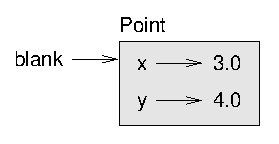
\includegraphics{figs/point.eps}}
\afterfig

The variable {\tt blank} refers to a Point object, which
contains two attributes.  Each attribute refers to a
floating-point number.

You can read the value of an attribute using the same syntax:

\beforeverb
\begin{verbatim}
>>> print blank.y
4.0
>>> x = blank.x
>>> print x
3.0
\end{verbatim}
\afterverb
%
The expression {\tt blank.x} means, ``Go to the object {\tt blank}
refers to and get the value of {\tt x}.'' In this case, we assign that
value to a variable named {\tt x}.  There is no conflict between
the variable {\tt x} and the attribute {\tt x}.

You can use dot notation as part of any expression.  For example:

\beforeverb
\begin{verbatim}
>>> print '(%g, %g)' % (blank.x, blank.y)
(3.0, 4.0)
>>> distance = math.sqrt(blank.x**2 + blank.y**2)
>>> print distance
5.0
\end{verbatim}
\afterverb
%
You can pass an instance as an argument in the usual way.
For example:

\index{instance!as argument}

\beforeverb
\begin{verbatim}
def print_point(p):
    print '(%g, %g)' % (p.x, p.y)
\end{verbatim}
\afterverb
%
\verb"print_point" takes a point as an argument and displays it in
mathematical notation.  To invoke it, you can pass {\tt blank} as
an argument:

\beforeverb
\begin{verbatim}
>>> print_point(blank)
(3.0, 4.0)
\end{verbatim}
\afterverb
%
Inside the function, {\tt p} is an alias for {\tt blank}, so if
the function modifies {\tt p}, {\tt blank} changes.

\index{aliasing}


\begin{ex}
Write a function called {\tt distance} that takes two Points
as arguments and returns the distance between them.
\end{ex}



\section{Rectangles}

Sometimes it is obvious what the attributes of an object should be,
but other times you have to make decisions.  For example, imagine you
are designing a class to represent rectangles.  What attributes would
you use to specify the location and size of a rectangle?  You can
ignore angle; to keep things simple, assume that the rectangle is
either vertical or horizontal.

\index{representation}

There are at least two possibilities: 

\begin{itemize}

\item You could specify one corner of the rectangle
(or the center), the width, and the height.

\item You could specify two opposing corners.

\end{itemize}

At this point it is hard to say whether either is better than
the other, so we'll implement the first one, just as an example.

\index{Rectangle class}
\index{class!Rectangle}

Here is the class definition:

\beforeverb
\begin{verbatim}
class Rectangle(object):
    """represent a rectangle. 
       attributes: width, height, corner.
    """
\end{verbatim}
\afterverb
%
The docstring lists the attributes:  {\tt width} and
{\tt height} are numbers; {\tt corner} is a Point object that
specifies the lower-left corner.

To represent a rectangle, you have to instantiate a Rectangle
object and assign values to the attributes:

\beforeverb
\begin{verbatim}
box = Rectangle()
box.width = 100.0
box.height = 200.0
box.corner = Point()
box.corner.x = 0.0
box.corner.y = 0.0
\end{verbatim}
\afterverb
%
The expression {\tt box.corner.x} means,
``Go to the object {\tt box} refers to and select the attribute named
{\tt corner}; then go to that object and select the attribute named
{\tt x}.''

The figure shows the state of this object:

\index{state diagram}
\index{diagram!state}
\index{object diagram}
\index{diagram!object}

\beforefig
\centerline{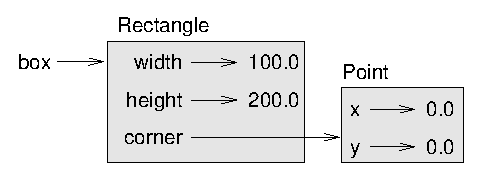
\includegraphics{figs/rectangle.eps}}
\afterfig

An object that is an attribute of another object is {\bf embedded}.

\index{embedded object}
\index{object!embedded}


\section{Instances as return values}

\index{instance!as return value}
\index{return value}

Functions can return instances.  For example, \verb"find_center"
takes a {\tt Rectangle} as an argument and returns a {\tt Point}
that contains the coordinates of the center of the {\tt Rectangle}:

\beforeverb
\begin{verbatim}
def find_center(box):
    p = Point()
    p.x = box.corner.x + box.width/2.0
    p.y = box.corner.y + box.height/2.0
    return p
\end{verbatim}
\afterverb
%
Here is an example that passes {\tt box} as an argument and assigns
the resulting Point to {\tt center}:

\beforeverb
\begin{verbatim}
>>> center = find_center(box)
>>> print_point(center)
(50.0, 100.0)
\end{verbatim}
\afterverb
%

\section{Objects are mutable}

\index{object!mutable}
\index{mutability}

You can change the state of an object by making an assignment to one of
its attributes.  For example, to change the size of a rectangle
without changing its position, you can modify the values of {\tt
width} and {\tt height}:

\beforeverb
\begin{verbatim}
box.width = box.width + 50
box.height = box.width + 100
\end{verbatim}
\afterverb
%
You can also write functions that modify objects.  For example,
\verb"grow_rectangle" takes a Rectangle object and two numbers,
{\tt dwidth} and {\tt dheight}, and adds the numbers to the
width and height of the rectangle:

\beforeverb
\begin{verbatim}
def grow_rectangle(rect, dwidth, dheight) :
    rect.width += dwidth
    rect.height += dheight
\end{verbatim}
\afterverb
%
Here is an example that demonstrates the effect:

\beforeverb
\begin{verbatim}
>>> print box.width
100.0
>>> print box.height
200.0
>>> grow_rectangle(box, 50, 100)
>>> print box.width
150.0
>>> print box.height
300.0
\end{verbatim}
\afterverb
%
Inside the function, {\tt rect} is an
alias for {\tt box}, so if the function modifies {\tt rect}, 
{\tt box} changes.

\begin{ex}
Write a function named \verb"move_rectangle" that takes
a Rectangle and two numbers named {\tt dx} and {\tt dy}.  It
should change the location of the rectangle by adding {\tt dx}
to the {\tt x} coordinate of {\tt corner} and adding {\tt dy}
to the {\tt y} coordinate of {\tt corner}.
\end{ex}


\section{Copying}

\index{aliasing}

Aliasing can make a program difficult to read because changes
in one place might have unexpected effects in another place.
It is hard to keep track of all the variables that might refer
to a given object.

\index{copying objects}
\index{object!copying}
\index{copy module}
\index{module!copy}

Copying an object is often an alternative to aliasing.
The {\tt copy} module contains a function called {\tt copy} that
can duplicate any object:

\beforeverb
\begin{verbatim}
>>> p1 = Point()
>>> p1.x = 3.0
>>> p1.y = 4.0

>>> import copy
>>> p2 = copy.copy(p1)
\end{verbatim}
\afterverb
%
{\tt p1} and {\tt p2} contain the same data, but they are
not the same Point.

\beforeverb
\begin{verbatim}
>>> print_point(p1)
(3.0, 4.0)
>>> print_point(p2)
(3.0, 4.0)
>>> p1 is p2
False
>>> p1 == p2
False
\end{verbatim}
\afterverb
%
The {\tt is} operator indicates that {\tt p1} and {\tt p2} are not the
same object, which is what we expected.  But you might have expected
{\tt ==} to yield {\tt True} because these points contain the same
data.  In that case, you will be disappointed to learn that for
instances, the default behavior of the {\tt ==} operator is the same
as the {\tt is} operator; it checks object identity, not object
equivalence.  This behavior can be changed---we'll see how later.

\index{is operator}
\index{operator!is}

If you use {\tt copy.copy} to duplicate a Rectangle, you will find
that it copies the Rectangle object but not the embedded Point.

\index{embedded object!copying}

\beforeverb
\begin{verbatim}
>>> box2 = copy.copy(box)
>>> box2 is box
False
>>> box2.corner is box.corner
True
\end{verbatim}
\afterverb
%
Here is what the object diagram looks like:

\index{state diagram}
\index{diagram!state}
\index{object diagram}
\index{diagram!object}

\vspace{0.1in}
\beforefig
\centerline{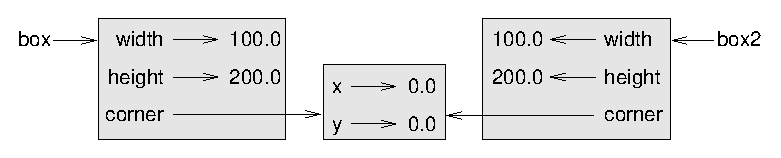
\includegraphics{figs/rectangle2.eps}}
\afterfig
\vspace{0.1in}

This operation is called a {\bf shallow copy} because it copies the
object and any references it contains, but not the embedded objects.

\index{shallow copy}
\index{copy!shallow}

For most applications, this is not what you want.  In this example,
invoking \verb"grow_rectangle" on one of the Rectangles would not
affect the other, but invoking \verb"move_rectangle" on either would
affect both!  This behavior is confusing and error-prone.

\index{deep copy}
\index{copy!deep}

Fortunately, the {\tt copy} module contains a method named {\tt
deepcopy} that copies not only the object but also 
the objects it refers to, and the objects {\em they} refer to,
and so on.
You will not be surprised to learn that this operation is
called a {\bf deep copy}.

\index{deepcopy function}
\index{function!deepcopy}

\beforeverb
\begin{verbatim}
>>> box3 = copy.deepcopy(box)
>>> box3 is box
False
>>> box3.corner is box.corner
False
\end{verbatim}
\afterverb
%
{\tt box3} and {\tt box} are completely separate objects.


\begin{ex}
Write a version of \verb"move_rectangle" that creates and
returns a new Rectangle instead of modifying the old one.
\end{ex}


\section{Debugging}
\label{hasattr}

\index{debugging}

When you start working with objects, you are likely to encounter
some new exceptions.  If you try to access an attribute
that doesn't exist, you get an {\tt AttributeError}:

\index{exception!AttributeError}
\index{AttributeError}

\beforeverb
\begin{verbatim}
>>> p = Point()
>>> print p.z
AttributeError: Point instance has no attribute 'z'
\end{verbatim}
\afterverb
%
If you are not sure what type an object is, you can ask:

\index{type function}
\index{function!type}

\beforeverb
\begin{verbatim}
>>> type(p)
<type '__main__.Point'>
\end{verbatim}
\afterverb
%
If you are not sure whether an object has a particular attribute,
you can use the built-in function {\tt hasattr}:

\index{hasattr function}
\index{function!hasattr}

\beforeverb
\begin{verbatim}
>>> hasattr(p, 'x')
True
>>> hasattr(p, 'z')
False
\end{verbatim}
\afterverb
%
The first argument can be any object; the second argument is a {\em
string} that contains the name of the attribute.


\section{Glossary}

\begin{description}

\item[class:] A user-defined type.  A class definition creates a new
class object.
\index{class}

\item[class object:] An object that contains information about a
user-defined type.  The class object can be used to create instances
of the type.
\index{class object}

\item[instance:] An object that belongs to a class.
\index{instance}

\item[attribute:] One of the named values associated with an object.
\index{attribute!instance}
\index{instance attribute}

\item[embedded (object):] An object that is stored as an attribute
of another object.
\index{embedded object}
\index{object!embedded}

\item[shallow copy:] To copy the contents of an object, including
any references to embedded objects;
implemented by the {\tt copy} function in the {\tt copy} module.
\index{shallow copy}

\item[deep copy:] To copy the contents of an object as well as any
embedded objects, and any objects embedded in them, and so on;
implemented by the {\tt deepcopy} function in the {\tt copy} module.
\index{deep copy}

\item[object diagram:] A diagram that shows objects, their
attributes, and the values of the attributes.
\index{object diagram}
\index{diagram!object}

\end{description}


\section{Exercises}

\begin{ex}
\label{canvas}

\index{Swampy}
\index{World module}
\index{module!World}

{\tt World.py}, which is part of Swampy (see Chapter~\ref{turtlechap}),
contains a class definition for a user-defined type called 
{\tt World}.  You can import it like this:

\beforeverb
\begin{verbatim}
from World import World
\end{verbatim}
\afterverb

This version of the {\tt import} statement imports the {\tt World}
class from the {\tt World} module.
The following code creates a World object and calls
the {\tt mainloop} method, which
waits for
the user.

\beforeverb
\begin{verbatim}
world = World()
world.mainloop()
\end{verbatim}
\afterverb

A window should appear with a title bar and an empty square.
We will use this window to draw Points,
Rectangles and other shapes.  
Add the following lines before calling
\verb"mainloop" and run the program again.

\index{Canvas object}
\index{object!Canvas}

\beforeverb
\begin{verbatim}
canvas = world.ca(width=500, height=500, background='white')
bbox = [[-150,-100], [150, 100]]
canvas.rectangle(bbox, outline='black', width=2, fill='green4')
\end{verbatim}
\afterverb

You should see a green rectangle with a black outline.
The first line creates a Canvas, which appears in the window
as a white square.  The Canvas object provides methods like
{\tt rectangle} for drawing various shapes.

\index{bounding box}

{\tt bbox} is a list of lists that represents the ``bounding box''
of the rectangle.  The first pair of coordinates is the lower-left
corner of the rectangle; the second pair is the upper-right corner.

You can draw a circle like this:

\beforeverb
\begin{verbatim}
canvas.circle([-25,0], 70, outline=None, fill='red')
\end{verbatim}
\afterverb

\index{Bangladesh, national flag}

The first parameter is the coordinate pair for the center of the
circle; the second parameter is the radius.

If you add this line to the program, 
the result should resemble the national flag of Bangladesh
(see \url{wikipedia.org/wiki/Gallery_of_sovereign-state_flags}).

\begin{enumerate}

\item Write a function called \verb"draw_rectangle" that takes a
  Canvas and a Rectangle as arguments and draws a
  representation of the Rectangle on the Canvas.

\item Add an attribute named {\tt color} to your Rectangle objects and
  modify \verb"draw_rectangle" so that it uses the color attribute as
  the fill color.

\item Write a function called \verb"draw_point" that takes a
  Canvas and a Point as arguments and draws a
  representation of the Point on the Canvas.

\item Define a new class called Circle with appropriate attributes and
  instantiate a few Circle objects.  Write a function called
  \verb"draw_circle" that draws circles on the canvas.

\index{Czech Republic, national flag}

\item Write a program that draws the national flag of the Czech Republic.
Hint: you can draw a polygon like this:

\beforeverb
\begin{verbatim}
points = [[-150,-100], [150, 100], [150, -100]]
canvas.polygon(points, fill='blue')
\end{verbatim}
\afterverb

\end{enumerate}

\index{color list}
\index{available colors}

I have written a small program that lists the available colors;
you can download it from \url{thinkpython.com/code/color_list.py}.

\end{ex}



\chapter{Classes and functions}
\label{time}


\section{Time}

As another example of a user-defined type, we'll define a class called
{\tt Time} that records the time of day.  The class definition looks
like this:

\index{user-defined type}
\index{type!user-defined}
\index{Time class}
\index{class!Time}

\beforeverb
\begin{verbatim}
class Time(object):
    """represents the time of day.
       attributes: hour, minute, second"""
\end{verbatim}
\afterverb
%
We can create a new {\tt Time} object and assign
attributes for hours, minutes, and seconds:

\beforeverb
\begin{verbatim}
time = Time()
time.hour = 11
time.minute = 59
time.second = 30
\end{verbatim}
\afterverb
%
The state diagram for the {\tt Time} object looks like this:

\index{state diagram}
\index{diagram!state}
\index{object diagram}
\index{diagram!object}

\beforefig
\centerline{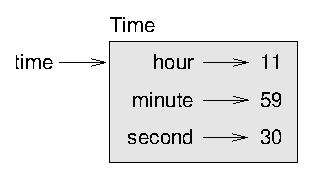
\includegraphics{figs/time.eps}}
\afterfig

\begin{ex}
\label{printtime}
Write a function called \verb"print_time" that takes a 
Time object and prints it in the form {\tt hour:minute:second}.
Hint: the format sequence \verb"'%.2d'" prints an integer using
at least two digits, including a leading zero if necessary.
\end{ex}

\begin{ex}
\label{is_after}

\index{boolean function}

Write a boolean function called \verb"is_after" that
takes two Time objects, {\tt t1} and {\tt t2}, and
returns {\tt True} if {\tt t1} follows {\tt t2} chronologically and
{\tt False} otherwise.  Challenge: don't use an {\tt if} statement.
\end{ex}


\section{Pure functions}

\index{prototype and patch}
\index{development plan!prototype and patch}

In the next few sections, we'll write two functions that add time
values.  They demonstrate two kinds of functions: pure functions and
modifiers.  They also demonstrate a development plan I'll call {\bf
  prototype and patch}, which is a way of tackling a complex problem
by starting with a simple prototype and incrementally dealing with the
complications.

Here is a simple prototype of \verb"add_time":

\beforeverb
\begin{verbatim}
def add_time(t1, t2):
    sum = Time()
    sum.hour = t1.hour + t2.hour
    sum.minute = t1.minute + t2.minute
    sum.second = t1.second + t2.second
    return sum
\end{verbatim}
\afterverb
%
The function creates a new {\tt Time} object, initializes its
attributes, and returns a reference to the new object.  This is called
a {\bf pure function} because it does not modify any of the objects
passed to it as arguments and it has no effect,
like displaying a value or getting user input, 
other than returning a value.

\index{pure function}
\index{function type!pure}

To test this function, I'll create two Time objects: {\tt start}
contains the start time of a movie, like {\em Monty Python and the
Holy Grail}, and {\tt duration} contains the run time of the movie,
which is one hour 35 minutes.

\index{Monty Python and the Holy Grail}

\verb"add_time" figures out when the movie will be done.

\beforeverb
\begin{verbatim}
>>> start = Time()
>>> start.hour = 9
>>> start.minute = 45
>>> start.second =  0

>>> duration = Time()
>>> duration.hour = 1
>>> duration.minute = 35
>>> duration.second = 0

>>> done = add_time(start, duration)
>>> print_time(done)
10:80:00
\end{verbatim}
\afterverb
%
The result, {\tt 10:80:00} might not be what you were hoping
for.  The problem is that this function does not deal with cases where the
number of seconds or minutes adds up to more than sixty.  When that
happens, we have to ``carry'' the extra seconds into the minute column
or the extra minutes into the hour column.

\index{carrying, addition with}

Here's an improved version:

\beforeverb
\begin{verbatim}
def add_time(t1, t2):
    sum = Time()
    sum.hour = t1.hour + t2.hour
    sum.minute = t1.minute + t2.minute
    sum.second = t1.second + t2.second

    if sum.second >= 60:
        sum.second -= 60
        sum.minute += 1

    if sum.minute >= 60:
        sum.minute -= 60
        sum.hour += 1

    return sum
\end{verbatim}
\afterverb
%
Although this function is correct, it is starting to get big.
We will see a shorter alternative later.


\section{Modifiers}
\label{increment}

\index{modifier}
\index{function type!modifier}

Sometimes it is useful for a function to modify the objects it gets as
parameters.  In that case, the changes are visible to the caller.
Functions that work this way are called {\bf modifiers}.

\index{increment}

{\tt increment}, which adds a given number of seconds to a {\tt Time}
object, can be written naturally as a
modifier.  Here is a rough draft:

\beforeverb
\begin{verbatim}
def increment(time, seconds):
    time.second += seconds

    if time.second >= 60:
        time.second -= 60
        time.minute += 1

    if time.minute >= 60:
        time.minute -= 60
        time.hour += 1
\end{verbatim}
\afterverb
%
The first line performs the basic operation; the remainder deals
with the special cases we saw before.

\index{special case}

Is this function correct?  What happens if the parameter {\tt seconds}
is much greater than sixty?  

In that case, it is not enough to carry
once; we have to keep doing it until {\tt time.second} is less than sixty.
One solution is to replace the {\tt if} statements with {\tt while}
statements.  That would make the function correct, but not
very efficient.

\begin{ex}
Write a correct version of {\tt increment} that
doesn't contain any loops.
\end{ex}

Anything that can be done with modifiers can also be done with pure
functions.  In fact, some programming languages only allow pure
functions.  There is some evidence that programs that use pure
functions are faster to develop and less error-prone than programs
that use modifiers.  But modifiers are convenient at times,
and functional programs tend to be less efficient.

In general, I recommend that you write pure functions whenever it is
reasonable and resort to modifiers only if there is a compelling
advantage.  This approach might be called a {\bf functional
programming style}.

\index{functional programming style}


\begin{ex}
Write a ``pure'' version of {\tt increment} that creates and returns
a new Time object rather than modifying the parameter.
\end{ex}


\section{Prototyping versus planning}
\label{prototype}

\index{prototype and patch}
\index{development plan!prototype and patch}
\index{planned development}
\index{development plan!planned}

The development plan I am demonstrating is called ``prototype and
patch.''  For each function, I wrote a prototype that performed the
basic calculation and then tested it, patching errors along the
way.

This approach can be effective, especially if you don't yet have a
deep understanding of the problem.  But incremental corrections can
generate code that is unnecessarily complicated---since it deals with
many special cases---and unreliable---since it is hard to know if you
have found all the errors.

An alternative is {\bf planned development}, in which high-level
insight into the problem can make the programming much easier.  In
this case, the insight is that a Time object is really a three-digit
number in base 60 (see \url{wikipedia.org/wiki/Sexagesimal}.)!  The
{\tt second} attribute is the ``ones column,'' the {\tt minute}
attribute is the ``sixties column,'' and the {\tt hour} attribute is
the ``thirty-six hundreds column.''

\index{sexagesimal}

When we wrote \verb"add_time" and {\tt increment}, we were effectively
doing addition in base 60, which is why we had to carry from one
column to the next.

\index{carrying, addition with}

This observation suggests another approach to the whole problem---we
can convert Time objects to integers and take advantage of the fact
that the computer knows how to do integer arithmetic.  

Here is a function that converts Times to integers:

\beforeverb
\begin{verbatim}
def time_to_int(time):
    minutes = time.hour * 60 + time.minute
    seconds = minutes * 60 + time.second
    return seconds
\end{verbatim}
\afterverb
%
And here is the function that converts integers to Times
(recall that {\tt divmod} divides the first argument by the second
and returns the quotient and remainder as a tuple).

\index{divmod}

\beforeverb
\begin{verbatim}
def int_to_time(seconds):
    time = Time()
    minutes, time.second = divmod(seconds, 60)
    time.hour, time.minute = divmod(minutes, 60)
    return time
\end{verbatim}
\afterverb
%
You might have to think a bit, and run some tests, to convince
yourself that these functions are correct.  One way to test them is to
check that \verb"time_to_int(int_to_time(x)) == x" for many values of
{\tt x}.  This is an example of a consistency check.

\index{consistency check}

Once you are convinced they are correct, you can use them to 
rewrite \verb"add_time":

\beforeverb
\begin{verbatim}
def add_time(t1, t2):
    seconds = time_to_int(t1) + time_to_int(t2)
    return int_to_time(seconds)
\end{verbatim}
\afterverb
%
This version is shorter than the original, and easier to verify.

\begin{ex}
Rewrite {\tt increment} using \verb"time_to_int" and \verb"int_to_time".
\end{ex}

In some ways, converting from base 60 to base 10 and back is harder
than just dealing with times.  Base conversion is more abstract; our
intuition for dealing with time values is better.

But if we have the insight to treat times as base 60 numbers and make
the investment of writing the conversion functions (\verb"time_to_int"
and \verb"int_to_time"), we get a program that is shorter, easier to
read and debug, and more reliable.

It is also easier to add features later.  For example, imagine
subtracting two Times to find the duration between them.  The
na\"{\i}ve approach would be to implement subtraction with borrowing.
Using the conversion functions would be easier and more likely to be
correct.

\index{subtraction with borrowing}
\index{borrowing, subtraction with}
\index{generalization}

Ironically, sometimes making a problem harder (or more general) makes it
easier (because there are fewer special cases and fewer opportunities
for error).


\section{Debugging}
\index{debugging}

A Time object is well-formed if the values of {\tt minutes} and {\tt
seconds} are between 0 and 60 (including 0 but not 60) and if 
{\tt hours} is positive.  {\tt hours} and {\tt minutes} should be
integral values, but we might allow {\tt seconds} to have a
fraction part.

\index{invariant}

Requirements like these are called {\bf invariants} because
they should always be true.  To put it a different way, if they
are not true, then something has gone wrong.

Writing code to check your invariants can help you detect errors
and find their causes.  For example, you might have a function
like \verb"valid_time" that takes a Time object and returns
{\tt False} if it violates an invariant:

\beforeverb
\begin{verbatim}
def valid_time(time):
    if time.hours < 0 or time.minutes < 0 or time.seconds < 0:
        return False
    if time.minutes >= 60 or time.seconds >= 60:
        return False
    return True
\end{verbatim}
\afterverb
%
Then at the beginning of each function you could check the
arguments to make sure they are valid:

\index{raise statement}
\index{statement!raise}

\beforeverb
\begin{verbatim}
def add_time(t1, t2):
    if not valid_time(t1) or not valid_time(t2):
        raise ValueError, 'invalid Time object in add_time'
    seconds = time_to_int(t1) + time_to_int(t2)
    return int_to_time(seconds)
\end{verbatim}
\afterverb
%
Or you could use an {\tt assert} statement, which checks a given invariant
and raises an exception if it fails:

\index{assert statement}
\index{statement!assert}

\beforeverb
\begin{verbatim}
def add_time(t1, t2):
    assert valid_time(t1) and valid_time(t2)
    seconds = time_to_int(t1) + time_to_int(t2)
    return int_to_time(seconds)
\end{verbatim}
\afterverb
%
{\tt assert} statements are useful because they distinguish
code that deals with normal conditions from code
that checks for errors.


\section{Glossary}

\begin{description}

\item[prototype and patch:] A development plan that involves
writing a rough draft of a program, testing, and correcting errors as
they are found.
\index{prototype and patch}

\item[planned development:] A development plan that involves
high-level insight into the problem and more planning than incremental
development or prototype development.
\index{planned development}

\item[pure function:] A function that does not modify any of the objects it
receives as arguments.  Most pure functions are fruitful.
\index{pure function}

\item[modifier:] A function that changes one or more of the objects it
receives as arguments.  Most modifiers are fruitless.
\index{modifier}

\item[functional programming style:] A style of program design in which the
majority of functions are pure.
\index{functional programming style}

\item[invariant:] A condition that should always be true during the
execution of a program.
\index{invariant}

\end{description}


\section{Exercises}

\begin{ex}
Write a function called \verb"mul_time" that takes a Time object
and a number and returns a new Time object that contains
the product of the original Time and the number.

Then use \verb"mul_time" to write a function that takes a Time
object that represents the finishing time in a race, and a number
that represents the distance, and returns a Time object that represents
the average pace (time per mile).

\index{running pace}

\end{ex}

\begin{ex}

\index{Date class}
\index{class!Date}

Write a class definition for a Date object that has attributes {\tt
  day}, {\tt month} and {\tt year}.  Write a function called
\verb"increment_date" that takes a Date object, {\tt date} and an
integer, {\tt n}, and returns a new Date object that
represents the day {\tt n} days after {\tt date}.  Hint:
``Thirty days hath September...''  Challenge: does your function
deal with leap years correctly?  See \url{wikipedia.org/wiki/Leap_year}.

\end{ex}


\begin{ex}

\index{datetime module}
\index{module!datetime}

The {\tt datetime} module provides {\tt date} and {\tt time} objects
that are similar to the Date and Time objects in this chapter, but
they provide a rich set of methods and operators.  Read the
documentation at \url{docs.python.org/lib/datetime-date.html}.

\begin{enumerate}

\item Use the {\tt datetime} module to write a program that
gets the current date and prints the day of the week.

\index{birthday}

\item Write a program that takes a birthday as input
and prints the user's age and the number of days, hours,
minutes and seconds until their next birthday.
\end{enumerate}

\end{ex}


\chapter{Classes and methods}


\section{Object-oriented features}

\index{object-oriented programming}

Python is an {\bf object-oriented programming language}, which means
that it provides features that support object-oriented
programming.

It is not easy to define object-oriented programming, but we have
already seen some of its characteristics:

\begin{itemize}

\item Programs are made up of object definitions and function
definitions, and most of the computation is expressed in terms
of operations on objects.

\item Each object definition corresponds to some object or concept
in the real world, and the functions that operate on that object
correspond to the ways real-world objects interact.

\end{itemize}

For example, the {\tt Time} class defined in Chapter~\ref{time}
corresponds to the way people record the time of day, and the
functions we defined correspond to the kinds of things people do with
times.  Similarly, the {\tt Point} and {\tt Rectangle} classes
correspond to the mathematical concepts of a point and a rectangle.

So far, we have not taken advantage of the features Python provides to
support object-oriented programming.  These
features are not strictly necessary; most of them provide
alternative syntax for things we have already done.  But in many cases,
the alternative is more concise and more accurately conveys the
structure of the program.

For example, in the {\tt Time} program, there is no obvious
connection between the class definition and the function definitions
that follow.  With some examination, it is apparent that every function
takes at least one {\tt Time} object as an argument.

\index{method}
\index{function}

This observation is the motivation for {\bf methods}; a method is
a function that is associated with a particular class.
We have seen methods for strings, lists, dictionaries and tuples.
In this chapter, we will define methods for user-defined types.

\index{syntax}
\index{semantics}

Methods are semantically the same as functions, but there are
two syntactic differences:

\begin{itemize}

\item Methods are defined inside a class definition in order
to make the relationship between the class and the method explicit.

\item The syntax for invoking a method is different from the
syntax for calling a function.

\end{itemize}

In the next few sections, we will take the functions from the previous
two chapters and transform them into methods.  This transformation is
purely mechanical; you can do it simply by following a sequence of
steps.  If you are comfortable converting from one form to another,
you will be able to choose the best form for whatever you are doing.


\section{Printing objects}
\label{print_time}

\index{object!printing}

In Chapter~\ref{time}, we defined a class named
{\tt Time} and in Exercise~\ref{printtime}, you 
wrote a function named \verb"print_time":

\beforeverb
\begin{verbatim}
class Time(object):
    """represents the time of day.
       attributes: hour, minute, second"""

def print_time(time):
    print '%.2d:%.2d:%.2d' % (time.hour, time.minute, time.second)
\end{verbatim}
\afterverb
%
To call this function, you have to pass a {\tt Time} object as an
argument:

\beforeverb
\begin{verbatim}
>>> start = Time()
>>> start.hour = 9
>>> start.minute = 45
>>> start.second = 00
>>> print_time(start)
09:45:00
\end{verbatim}
\afterverb
%
To make \verb"print_time" a method, all we have to do is
move the function definition inside the class definition.  Notice
the change in indentation.

\index{indentation}

\beforeverb
\begin{verbatim}
class Time(object):
    def print_time(time):
        print '%.2d:%.2d:%.2d' % (time.hour, time.minute, time.second)
\end{verbatim}
\afterverb
%
Now there are two ways to call \verb"print_time".  The first
(and less common) way is to use function syntax:

\index{function syntax}
\index{dot notation}


\beforeverb
\begin{verbatim}
>>> Time.print_time(start)
09:45:00
\end{verbatim}
\afterverb
%
In this use of dot notation, {\tt Time} is the name of the class,
and \verb"print_time" is the name of the method.  {\tt start} is
passed as a parameter.

The second (and more concise) way is to use method syntax:

\index{method syntax}

\beforeverb
\begin{verbatim}
>>> start.print_time()
09:45:00
\end{verbatim}
\afterverb
%
In this use of dot notation, \verb"print_time" is the name of the
method (again), and {\tt start} is the object the method is
invoked on, which is called the {\bf subject}.  Just as the
subject of a sentence is what the sentence is about, the subject
of a method invocation is what the method is about.

\index{subject}

Inside the method, the subject is assigned to the first
parameter, so in this case {\tt start} is assigned
to {\tt time}.

\index{self (parameter name)}
\index{parameter!self}

By convention, the first parameter of a method is
called {\tt self}, so it would be more common to write
\verb"print_time" like this:

\beforeverb
\begin{verbatim}
class Time(object):
    def print_time(self):
        print '%.2d:%.2d:%.2d' % (self.hour, self.minute, self.second)
\end{verbatim}
\afterverb
%
The reason for this convention is an implicit metaphor:

\index{metaphor, method invocation}

\begin{itemize}

\item The syntax for a function call, \verb"print_time(start)",
  suggests that the function is the active agent.  It says something
  like, ``Hey \verb"print_time"!  Here's an object for you to print.''

\item In object-oriented programming, the objects are the active
  agents.  A method invocation like \verb"start.print_time()" says
  ``Hey {\tt start}!  Please print yourself.''

\end{itemize}

This change in perspective might be more polite, but it is not obvious
that it is useful.  In the examples we have seen so far, it may not
be.  But sometimes shifting responsibility from the functions onto the
objects makes it possible to write more versatile functions, and makes
it easier to maintain and reuse code.

\begin{ex}
\label{convert}
Rewrite \verb"time_to_int"
(from Section~\ref{prototype}) as a method.  It is probably not
appropriate to rewrite \verb"int_to_time" as a method; it's not
clear what object you would invoke it on!
\end{ex}


\section{Another example}

\index{increment}

Here's a version of {\tt increment} (from Section~\ref{increment})
rewritten as a method:

\beforeverb
\begin{verbatim}
# inside class Time:

    def increment(self, seconds):
        seconds += self.time_to_int()
        return int_to_time(seconds)
\end{verbatim}
\afterverb
%
This version assumes that \verb"time_to_int" is written
as a method, as in Exercise~\ref{convert}.  Also, note that
it is a pure function, not a modifier.

Here's how you would invoke {\tt increment}:

\beforeverb
\begin{verbatim}
>>> start.print_time()
09:45:00
>>> end = start.increment(1337)
>>> end.print_time()
10:07:17
\end{verbatim}
\afterverb
%
The subject, {\tt start}, gets assigned to the first parameter,
{\tt self}.  The argument, {\tt 1337}, gets assigned to the
second parameter, {\tt seconds}.

This mechanism can be confusing, especially if you make an error.
For example, if you invoke {\tt increment} with two arguments, you
get:

\index{exception!TypeError}
\index{TypeError}

\beforeverb
\begin{verbatim}
>>> end = start.increment(1337, 460)
TypeError: increment() takes exactly 2 arguments (3 given)
\end{verbatim}
\afterverb
%
The error message is initially confusing, because there are
only two arguments in parentheses.  But the subject is also
considered an argument, so all together that's three.


\section{A more complicated example}

\verb"is_after" (from Exercise~\ref{is_after}) is slightly more complicated
because it takes two Time objects as parameters.  In this case it is
conventional to name the first parameter {\tt self} and the second
parameter {\tt other}:

\index{other (parameter name)}
\index{parameter!other}

\beforeverb
\begin{verbatim}
# inside class Time:

    def is_after(self, other):
        return self.time_to_int() > other.time_to_int()
\end{verbatim}
\afterverb
%
To use this method, you have to invoke it on one object and pass
the other as an argument:

\beforeverb
\begin{verbatim}
>>> end.is_after(start)
True
\end{verbatim}
\afterverb
%
One nice thing about this syntax is that it almost reads
like English: ``end is after start?''


\section{The init method}

\index{init method}
\index{method!init}

The init method (short for ``initialization'') is
a special method that gets invoked when an object is instantiated.  
Its full name is \verb"__init__" (two underscore characters,
followed by {\tt init}, and then two more underscores).  An
init method for the {\tt Time} class might look like this:

\beforeverb
\begin{verbatim}
# inside class Time:

    def __init__(self, hour=0, minute=0, second=0):
        self.hour = hour
        self.minute = minute
        self.second = second
\end{verbatim}
\afterverb
%
It is common for the parameters of \verb"__init__"
to have the same names as the attributes.  The statement

\beforeverb
\begin{verbatim}
        self.hour = hour
\end{verbatim}
\afterverb
%
stores the value of the parameter {\tt hour} as an attribute
of {\tt self}.

\index{optional parameter}
\index{parameter!optional}
\index{default value}
\index{override}

The parameters are optional, so if you call {\tt Time} with
no arguments, you get the default values.

\beforeverb
\begin{verbatim}
>>> time = Time()
>>> time.print_time()
00:00:00
\end{verbatim}
\afterverb
%
If you provide one argument, it overrides {\tt hour}:

\beforeverb
\begin{verbatim}
>>> time = Time (9)
>>> time.print_time()
09:00:00
\end{verbatim}
\afterverb
%
If you provide two arguments, they override {\tt hour} and
{\tt minute}.

\beforeverb
\begin{verbatim}
>>> time = Time(9, 45)
>>> time.print_time()
09:45:00
\end{verbatim}
\afterverb
%
And if you provide three arguments, they override all three
default values.


\begin{ex}
\index{Point class}
\index{class!Point}

Write an init method for the {\tt Point} class that takes
{\tt x} and {\tt y} as optional parameters and assigns
them to the corresponding attributes.
\end{ex}


\section{The {\tt \_\_str\_\_} method}

\index{str method@\_\_str\_\_ method}
\index{method!\_\_str\_\_}

\verb"__str__" is a special method, like \verb"__init__",
that is supposed to return a string representation of an object.

\index{string representation}

For example, here is a {\tt str} method for Time objects:

\beforeverb
\begin{verbatim}
# inside class Time:

    def __str__(self):
        return '%.2d:%.2d:%.2d' % (self.hour, self.minute, self.second)
\end{verbatim}
\afterverb
%
When you {\tt print} an object, Python invokes the {\tt str} method:

\index{print statement}
\index{statement!print}

\beforeverb
\begin{verbatim}
>>> time = Time(9, 45)
>>> print time
09:45:00
\end{verbatim}
\afterverb
%
When I write a new class, I almost always start by writing 
\verb"__init__", which makes it easier to instantiate objects, and 
\verb"__str__", which is useful for debugging.


\begin{ex}
Write a {\tt str} method for the {\tt Point} class.  Create
a Point object and print it.
\end{ex}


\section{Operator overloading}
\label{operator overloading}

By defining other special methods, you can specify the behavior
of operators on user-defined types.  For example, if you define
a method named \verb"__add__" for the {\tt Time} class, you can use the
{\tt +} operator on Time objects.

Here is what the definition might look like:

\index{add method}
\index{method!add}

\beforeverb
\begin{verbatim}
# inside class Time:

    def __add__(self, other):
        seconds = self.time_to_int() + other.time_to_int()
        return int_to_time(seconds)
\end{verbatim}
\afterverb
%
And here is how you could use it:

\beforeverb
\begin{verbatim}
>>> start = Time(9, 45)
>>> duration = Time(1, 35)
>>> print start + duration
11:20:00
\end{verbatim}
\afterverb
%
When you apply the {\tt +} operator to Time objects, Python invokes
\verb"__add__".  When you print the result, Python invokes 
\verb"__str__".  So there is quite a lot happening behind the scenes!

\index{operator overloading}

Changing the behavior of an operator so that it works with
user-defined types is called {\bf operator overloading}.  For every
operator in Python there is a corresponding special method, like 
\verb"__add__".  For more details, see
\url{docs.python.org/ref/specialnames.html}.

\begin{ex}
Write an {\tt add} method for the Point class.  
\end{ex}


\section{Type-based dispatch}

In the previous section we added two Time objects, but you
also might want to add an integer to a Time object.  The
following is a version of \verb"__add__"
that checks the type of {\tt other} and invokes either
\verb"add_time" or {\tt increment}:

\beforeverb
\begin{verbatim}
# inside class Time:

    def __add__(self, other):
        if isinstance(other, Time):
            return self.add_time(other)
        else:
            return self.increment(other)

    def add_time(self, other):
        seconds = self.time_to_int() + other.time_to_int()
        return int_to_time(seconds)

    def increment(self, seconds):
        seconds += self.time_to_int()
        return int_to_time(seconds)
\end{verbatim}
\afterverb
%
The built-in function {\tt isinstance} takes a value and a
class object, and returns {\tt True} if the value is an instance
of the class.

\index{isinstance function}
\index{function!isinstance}

If {\tt other} is a Time object, \verb"__add__" invokes
\verb"add_time".  Otherwise it assumes that the parameter
is a number and invokes {\tt increment}.  This operation is
called a {\bf type-based dispatch} because it dispatches the
computation to different methods based on the type of the
arguments.

\index{type-based dispatch}
\index{dispatch, type-based}

Here are examples that use the {\tt +} operator with different
types:

\beforeverb
\begin{verbatim}
>>> start = Time(9, 45)
>>> duration = Time(1, 35)
>>> print start + duration
11:20:00
>>> print start + 1337
10:07:17
\end{verbatim}
\afterverb
%
Unfortunately, this implementation of addition is not commutative.
If the integer is the first operand, you get

\index{commutativity}

\beforeverb
\begin{verbatim}
>>> print 1337 + start
TypeError: unsupported operand type(s) for +: 'int' and 'instance'
\end{verbatim}
\afterverb
%
The problem is, instead of asking the Time object to add an integer,
Python is asking an integer to add a Time object, and it doesn't know
how to do that.  But there is a clever solution for this problem: the
special method \verb"__radd__", which stands for ``right-side add.''
This method is invoked when a Time object appears on the right side of
the {\tt +} operator.  Here's the definition:

\index{radd method}
\index{method!radd}

\beforeverb
\begin{verbatim}
# inside class Time:

    def __radd__(self, other):
        return self.__add__(other)
\end{verbatim}
\afterverb
%
And here's how it's used:

\beforeverb
\begin{verbatim}
>>> print 1337 + start
10:07:17
\end{verbatim}
\afterverb
%

\begin{ex}
Write an {\tt add} method for Points that works with either a
Point object or a tuple:  

\begin{itemize}

\item If the second operand is a Point, the method should return a new
Point whose $x$ coordinate is the sum of the $x$ coordinates of the
operands, and likewise for the $y$ coordinates.

\item If the second operand is a tuple, the method should add the
first element of the tuple to the $x$ coordinate and the second
element to the $y$ coordinate, and return a new Point with the result. 

\end{itemize}

\end{ex}

\section{Polymorphism}

Type-based dispatch is useful when it is necessary, but (fortunately)
it is not always necessary.  Often you can avoid it by writing functions
that work correctly for arguments with different types.

\index{type-based dispatch}
\index{dispatch!type-based}

Many of the functions we wrote for strings will actually
work for any kind of sequence.
For example, in Section~\ref{histogram}
we used {\tt histogram} to count the number of times each letter
appears in a word.

\beforeverb
\begin{verbatim}
def histogram(s):
    d = dict()
    for c in s:
        if c not in d:
            d[c] = 1
        else:
            d[c] = d[c]+1
    return d
\end{verbatim}
\afterverb
%
This function also works for lists, tuples, and even dictionaries,
as long as the elements of {\tt s} are hashable, so they can be used
as keys in {\tt d}.

\beforeverb
\begin{verbatim}
>>> t = ['spam', 'egg', 'spam', 'spam', 'bacon', 'spam']
>>> histogram(t)
{'bacon': 1, 'egg': 1, 'spam': 4}
\end{verbatim}
\afterverb
%
Functions that can work with several types are called {\bf polymorphic}.
Polymorphism can facilitate code reuse.  For example, the built-in
function {\tt sum}, which adds the elements of a sequence, works
as long as the elements of the sequence support addition.

\index{polymorphism}

Since Time objects provide an {\tt add} method, they work
with {\tt sum}:

\beforeverb
\begin{verbatim}
>>> t1 = Time(7, 43)
>>> t2 = Time(7, 41)
>>> t3 = Time(7, 37)
>>> total = sum([t1, t2, t3])
>>> print total
23:01:00
\end{verbatim}
\afterverb
%
In general, if all of the operations inside a function 
work with a given type, then the function works with that type.

The best kind of polymorphism is the unintentional kind, where
you discover that a function you already wrote can be
applied to a type you never planned for.


\section{Debugging}
\index{debugging}

It is legal to add attributes to objects at any point in the execution
of a program, but if you are a stickler for type theory, it is a
dubious practice to have objects of the same type with different
attribute sets.  It is usually a good idea to
initialize all of an objects attributes in the init method.

\index{init method}
\index{attribute!initializing}

If you are not sure whether an object has a particular attribute, you
can use the built-in function {\tt hasattr} (see Section~\ref{hasattr}).

\index{hasattr function}
\index{function!hasattr}
\index{dict attribute@\_\_dict\_\_ attribute}
\index{attribute!\_\_dict\_\_}

Another way to access the attributes of an object is through the
special attribute \verb"__dict__", which is a dictionary that maps
attribute names (as strings) and values:

\beforeverb
\begin{verbatim}
>>> p = Point(3, 4)
>>> print p.__dict__
{'y': 4, 'x': 3}
\end{verbatim}
\afterverb
%
For purposes of debugging, you might find it useful to keep this
function handy:

\beforeverb
\begin{verbatim}
def print_attributes(obj):
    for attr in obj.__dict__:
        print attr, getattr(obj, attr)
\end{verbatim}
\afterverb
%
\verb"print_attributes" traverses the items in the object's dictionary
and prints each attribute name and its corresponding value.

\index{traversal!dictionary}
\index{dictionary!traversal}

The built-in function {\tt getattr} takes an object and an attribute
name (as a string) and returns the attribute's value.

\index{getattr function}
\index{function!getattr}


\section{Glossary}

\begin{description}

\item[object-oriented language:] A language that provides features,
  such as user-defined classes and method syntax, that facilitate
  object-oriented programming.
\index{object-oriented language}

\item[object-oriented programming:] A style of programming in which
data and the operations that manipulate it are organized into classes
and methods.
\index{object-oriented programming}

\item[method:] A function that is defined inside a class definition and
is invoked on instances of that class.
\index{method}

\item[subject:] The object a method is invoked on.
\index{subject}

\item[operator overloading:] Changing the behavior of an operator like
{\tt +} so it works with a user-defined type.
\index{overloading}
\index{operator!overloading}

\item[type-based dispatch:] A programming pattern that checks the type
of an operand and invokes different functions for different types.
\index{type-based dispatch}

\item[polymorphic:] Pertaining to a function that can work with more
  than one type.  

\index{polymorphism}

\end{description}

\section{Exercises}

\begin{ex}

\index{default value!avoiding mutable}
\index{mutable object, as default value}
\index{worst bug}
\index{bug!worst}

This exercise is a cautionary tale about one of the most
common, and difficult to find, errors in Python.

\begin{enumerate}

\index{Kangaroo class}
\index{class!Kangaroo}

\item Write a definition for a class named {\tt Kangaroo} with the following
methods:

\begin{enumerate}

\item An \verb"__init__" method that initializes an attribute named 
\verb"pouch_contents" to an empty list.

\item A method named \verb"put_in_pouch" that takes an object
of any type and adds it to \verb"pouch_contents".

\item A \verb"__str__" method that returns a string representation
of the Kangaroo object and the contents of the pouch.

\end{enumerate}
%
Test your code 
by creating two {\tt Kangaroo} objects, assigning them to variables
named {\tt kanga} and {\tt roo}, and then adding {\tt roo} to the
contents of {\tt kanga}'s pouch.

\item Download \url{thinkpython.com/code/BadKangaroo.py}.  It contains
a solution to the previous problem with one big, nasty bug.
Find and fix the bug.

If you get stuck, you can download
\url{thinkpython.com/code/GoodKangaroo.py}, which explains the
problem and demonstrates a solution.

\index{aliasing}
\index{embedded object}
\index{object!embedded}

\end{enumerate}


\end{ex}




\begin{ex}

\index{Visual module}
\index{module!Visual}
\index{vpython module}
\index{module!vpython}

Visual is a Python module that provides 3-D graphics.  It is
not always included in a Python installation, so you might have
to install it from your software repository or, if it's not there,
from \url{vpython.org}.

The following example creates a 3-D space that is 256 units
wide, long and high, and sets the ``center'' to be the
point $(128, 128, 128)$.  Then it draws a blue sphere.

\beforeverb
\begin{verbatim}
from visual import *

scene.range = (256, 256, 256)
scene.center = (128, 128, 128)

color = (0.1, 0.1, 0.9)          # mostly blue
sphere(pos=scene.center, radius=128, color=color)
\end{verbatim}
\afterverb

{\tt color} is an RGB tuple; that is, the elements are Red-Green-Blue
levels between 0.0 and 1.0 (see
\url{wikipedia.org/wiki/RGB_color_model}).

If you run this code, you should see a window with a black
background and a blue sphere.  If you drag the middle button
up and down, you can zoom in and out.  You can also rotate
the scene by dragging the right button, but with only one
sphere in the world, it is hard to tell the difference.

The following loop creates a cube of spheres:

\beforeverb
\begin{verbatim}
t = range(0, 256, 51)
for x in t:
    for y in t:
        for z in t:
            pos = x, y, z
            sphere(pos=pos, radius=10, color=color)
\end{verbatim}
\afterverb

\begin{enumerate}

\item Put this code in a script and make sure it works for
you.

\item Modify the program so that each sphere in the cube
has the color that corresponds to its position in RGB space.
Notice that the coordinates are in the range 0--255, but
the RGB tuples are in the range 0.0--1.0.

\index{color list}
\index{available colors}

\item Download \url{thinkpython.com/code/color_list.py}
and use the function \verb"read_colors" to generate a list
of the available colors on your system, their names and
RGB values.  For each named color draw a sphere in the
position that corresponds to its RGB values.



\end{enumerate}

You can see my solution at \url{thinkpython.com/code/color_space.py}.

\end{ex}


\chapter{Inheritance}

In this chapter we will develop classes to represent playing cards,
decks of cards, and poker hands.  If you don't play poker, you can
read about it at \url{wikipedia.org/wiki/Poker}, but you don't have
to; I'll tell you what you need to know for the exercises.

\index{playing card, Anglo-American}
\index{card, playing}
\index{poker}

If you are not familiar with Anglo-American playing cards,
you can read about them at \url{wikipedia.org/wiki/Playing_cards}.


\section{Card objects}

There are fifty-two cards in a deck, each of which belongs to one of
four suits and one of thirteen ranks.  The suits are Spades, Hearts,
Diamonds, and Clubs (in descending order in bridge).  The ranks are
Ace, 2, 3, 4, 5, 6, 7, 8, 9, 10, Jack, Queen, and King.  Depending on
the game that you are playing, an Ace may be higher than King
or lower than 2.

\index{rank}
\index{suit}

If we want to define a new object to represent a playing card, it is
obvious what the attributes should be: {\tt rank} and
{\tt suit}.  It is not as obvious what type the attributes
should be.  One possibility is to use strings containing words like
\verb"'Spade'" for suits and \verb"'Queen'" for ranks.  One problem with
this implementation is that it would not be easy to compare cards to
see which had a higher rank or suit.

\index{encode}
\index{encrypt}
\index{map to}
\index{representation}

An alternative is to use integers to {\bf encode} the ranks and suits.
In this context, ``encode'' means that we are going to define a mapping
between numbers and suits, or between numbers and ranks.  This
kind of encoding is not meant to be a secret (that
would be ``encryption'').

For example, this table shows the suits and the corresponding integer
codes:

\beforefig
\begin{tabular}{l c l}
Spades & $\mapsto$ & 3 \\
Hearts & $\mapsto$ & 2 \\
Diamonds & $\mapsto$ & 1 \\
Clubs & $\mapsto$ & 0
\end{tabular}
\afterfig

This code makes it easy to compare cards; because higher suits map to
higher numbers, we can compare suits by comparing their codes.

The mapping for ranks is fairly obvious; each of the numerical ranks
maps to the corresponding integer, and for face cards:

\beforefig
\begin{tabular}{l c l}
Jack & $\mapsto$ & 11 \\
Queen & $\mapsto$ & 12 \\
King & $\mapsto$ & 13 \\
\end{tabular}
\afterfig

I am using the $\mapsto$ symbol to make it clear that these mappings
are not part of the Python program.  They are part of the program
design, but they don't appear explicitly in the code.

\index{Card class}
\index{class!Card}

The class definition for {\tt Card} looks like this:

\beforeverb
\begin{verbatim}
class Card(object):
    """represents a standard playing card."""

    def __init__(self, suit=0, rank=2):
        self.suit = suit
        self.rank = rank
\end{verbatim}
\afterverb
%
As usual, the init method takes an optional
parameter for each attribute.  The default card is
the 2 of Clubs.

\index{init method}
\index{method!init}

To create a Card, you call {\tt Card} with the
suit and rank of the card you want.

\beforeverb
\begin{verbatim}
queen_of_diamonds = Card(1, 12)
\end{verbatim}
\afterverb
%


\section{Class attributes}

\index{class attribute}
\index{attribute!class}

In order to print Card objects in a way that people can easily
read, we need a mapping from the integer codes to the corresponding
ranks and suits.  A natural way to
do that is with lists of strings.  We assign these lists to {\bf class
attributes}:

\beforeverb
\begin{verbatim}
# inside class Card:

    suit_names = ['Clubs', 'Diamonds', 'Hearts', 'Spades']
    rank_names = [None, 'Ace', '2', '3', '4', '5', '6', '7', 
              '8', '9', '10', 'Jack', 'Queen', 'King']

    def __str__(self):
        return '%s of %s' % (Card.rank_names[self.rank],
                             Card.suit_names[self.suit])
\end{verbatim}
\afterverb
%
Variables like \verb"suit_names" and \verb"rank_names", which are
defined inside a class but outside of any method, are called
class attributes because they are associated with the class object 
{\tt Card}.

\index{instance attribute}
\index{attribute!instance}

This term distinguishes them from variables like {\tt suit} and {\tt
  rank}, which are called {\bf instance attributes} because they are
associated with a particular instance.

\index{dot notation}

Both kinds of attribute are accessed using dot notation.  For
example, in \verb"__str__", {\tt self} is a Card object,
and {\tt self.rank} is its rank.  Similarly, {\tt Card}
is a class object, and \verb"Card.rank_names" is a
list of strings associated with the class.

Every card has its own {\tt suit} and {\tt rank}, but there
is only one copy of \verb"suit_names" and \verb"rank_names".

Putting it all together, the expression
\verb"Card.rank_names[self.rank]" means ``use the attribute {\tt rank}
from the object {\tt self} as an index into the list \verb"rank_names"
from the class {\tt Card}, and select the appropriate string.''

The first element of \verb"rank_names" is {\tt None} because there
is no card with rank zero.  By including {\tt None} as a place-keeper,
we get a mapping with the nice property that the index 2 maps to the
string \verb"'2'", and so on.  To avoid this tweak, we could have
used a dictionary instead of a list.

With the methods we have so far, we can create and print cards:

\beforeverb
\begin{verbatim}
>>> card1 = Card(2, 11)
>>> print card1
Jack of Hearts
\end{verbatim}
\afterverb
%
Here is a diagram that shows the {\tt Card} class object
and one Card instance:

\index{state diagram}
\index{diagram!state}
\index{object diagram}
\index{diagram!object}

\beforefig
\centerline{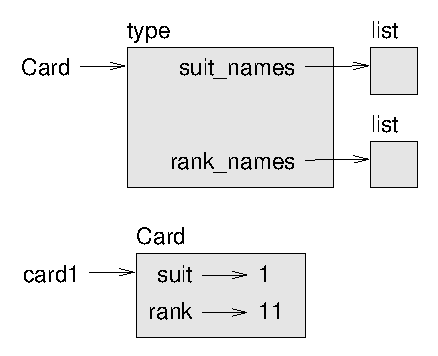
\includegraphics{figs/card1.eps}}
\afterfig

{\tt Card} is a class object, so it has type {\tt type}.  {\tt
card1} has type {\tt Card}.  (To save space, I didn't draw the
contents of \verb"suit_names" and \verb"rank_names").


\section{Comparing cards}
\label{comparecard}

\index{operator!relational}
\index{relational operator}

For built-in types, there are relational operators
({\tt <}, {\tt >}, {\tt ==}, etc.)
that compare
values and determine when one is greater than, less than, or equal to
another.  For user-defined types, we can override the behavior of
the built-in operators by providing a method named
\verb"__cmp__".  

\verb"__cmp__" takes two parameters, {\tt self} and {\tt other},
and returns a positive number if the first object is greater, a
negative number if the second object is greater, and 0 if they are
equal to each other.

\index{override}
\index{operator overloading}

The correct ordering for cards is not obvious.
For example, which
is better, the 3 of Clubs or the 2 of Diamonds?  One has a higher
rank, but the other has a higher suit.  In order to compare
cards, you have to decide whether rank or suit is more important.

The answer might depend on what game you are playing, but to keep
things simple, we'll make the arbitrary choice that suit is more
important, so all of the Spades outrank all of the Diamonds,
and so on.

\index{cmp method@\_\_cmp\_\_ method}
\index{method!\_\_cmp\_\_}

With that decided, we can write \verb"__cmp__":

\beforeverb
\begin{verbatim}
# inside class Card:

    def __cmp__(self, other):
        # check the suits
        if self.suit > other.suit: return 1
        if self.suit < other.suit: return -1

        # suits are the same... check ranks
        if self.rank > other.rank: return 1
        if self.rank < other.rank: return -1

        # ranks are the same... it's a tie
        return 0    
\end{verbatim}
\afterverb
%
You can write this more concisely using tuple comparison:

\index{tuple!comparison}
\index{comparison!tuple}

\beforeverb
\begin{verbatim}
# inside class Card:

    def __cmp__(self, other):
        t1 = self.suit, self.rank
        t2 = other.suit, other.rank
        return cmp(t1, t2)
\end{verbatim}
\afterverb
%
The built-in function {\tt cmp} has the same interface as
the method \verb"__cmp__": it takes two values and returns
a positive number if the first is larger, a negative number
if the second is larger, and 0 if they are equal.

\index{cmp function}
\index{function!cmp}


\begin{ex}
Write a \verb"__cmp__" method for Time objects.  Hint: you
can use tuple comparison, but you also might consider using
integer subtraction.

%    def __cmp__(self, other):
%        return time_to_int(self) - time_to_int(other)

%If {\tt self} is later than {\tt other}, the result is
%a positive number.  If {\tt other} is later, the result
%is negative.  And if {\tt self} and {\tt other} are equal
%(but not necessarily identical)
%the result is zero.

\end{ex}


\section{Decks}
\index{list!of objects}
\index{deck, playing cards}

Now that we have Cards, the next step is to define Decks.  Since a
deck is made up of cards, it is natural for each Deck to contain a
list of cards as an attribute.

\index{init method}
\index{method!init}

The following is a class definition for {\tt Deck}.  The
init method creates the attribute {\tt cards} and generates
the standard set of fifty-two cards:

\index{composition}
\index{loop!nested}

\index{Deck class}
\index{class!Deck}

\beforeverb
\begin{verbatim}
class Deck(object):

    def __init__(self):
        self.cards = []
        for suit in range(4):
            for rank in range(1, 14):
                card = Card(suit, rank)
                self.cards.append(card)
\end{verbatim}
\afterverb
%
The easiest way to populate the deck is with a nested loop.  The outer
loop enumerates the suits from 0 to 3.  The inner loop enumerates the
ranks from 1 to 13.  Each iteration
creates a new Card with the current suit and rank,
and appends it to {\tt self.cards}.

\index{append method}
\index{method!append}


\section{Printing the deck}
\label{printdeck}

\index{str method@\_\_str\_\_ method}
\index{method!\_\_str\_\_}

Here is a \verb"__str__" method for {\tt Deck}:

\beforeverb
\begin{verbatim}
#inside class Deck:

    def __str__(self):
        res = []
        for card in self.cards:
            res.append(str(card))
        return '\n'.join(res)
\end{verbatim}
\afterverb
%
This method demonstrates an efficient way to accumulate a large
string: building a list of strings and then using {\tt join}.
The built-in function {\tt str} invokes the \verb"__str__"
method on each card and returns the string representation.

\index{accumulator!string}
\index{string!accumulator}
\index{join method}
\index{method!join}
\index{newline}

Since we invoke {\tt join} on a newline character, the cards
are separated by newlines.  Here's what the result looks like:

\beforeverb
\begin{verbatim}
>>> deck = Deck()
>>> print deck
Ace of Clubs
2 of Clubs
3 of Clubs
...
10 of Spades
Jack of Spades
Queen of Spades
King of Spades
\end{verbatim}
\afterverb
%
Even though the result appears on 52 lines, it is
one long string that contains newlines.


\section{Add, remove, shuffle and sort}

To deal cards, we would like a method that
removes a card from the deck and returns it.
The list method {\tt pop} provides a convenient way to do that:

\index{pop method}
\index{method!pop}

\beforeverb
\begin{verbatim}
#inside class Deck:

    def pop_card(self):
        return self.cards.pop()
\end{verbatim}
\afterverb
%
Since {\tt pop} removes the {\em last} card in the list, we are
dealing from the bottom of the deck.  In real life bottom dealing is
frowned upon\footnote{See \url{wikipedia.org/wiki/Bottom_dealing}},
but in this context it's ok.

\index{append method}
\index{method!append}

To add a card, we can use the list method {\tt append}:

\beforeverb
\begin{verbatim}
#inside class Deck:

    def add_card(self, card):
        self.cards.append(card)
\end{verbatim}
\afterverb
%
A method like this that uses another function without doing
much real work is sometimes called a {\bf veneer}.  The metaphor
comes from woodworking, where it is common to glue a thin
layer of good quality wood to the surface of a cheaper piece of
wood.

\index{veneer}

In this case we are defining a ``thin'' method that expresses
a list operation in terms that are appropriate for decks.

As another example, we can write a Deck method named {\tt shuffle}
using the function {\tt shuffle} from the {\tt random} module:

\index{random module}
\index{module!random}
\index{shuffle function}
\index{function!shuffle}

\beforeverb
\begin{verbatim}
# inside class Deck:
            
    def shuffle(self):
        random.shuffle(self.cards)
\end{verbatim}
\afterverb
%
Don't forget to import {\tt random}.

\begin{ex}
\index{sort method}
\index{method!sort}

Write a Deck method named {\tt sort} that uses the list method
{\tt sort} to sort the cards in a {\tt Deck}.  {\tt sort} uses
the \verb"__cmp__" method we defined to determine sort order.
\end{ex}



\section{Inheritance}

\index{inheritance}
\index{object-oriented programming}

The language feature most often associated with object-oriented
programming is {\bf inheritance}.  Inheritance is the ability to
define a new class that is a modified version of an existing
class.

\index{parent class}
\index{child class}
\index{class!child}
\index{subclass}
\index{superclass}

It is called ``inheritance'' because the new class inherits the
methods of the existing class.  Extending this metaphor, the existing
class is called the {\bf parent} and the new class is
called the {\bf child}.

As an example, let's say we want a class to represent a ``hand,''
that is, the set of cards held by one player.  A hand is similar to a
deck: both are made up of a set of cards, and both require operations
like adding and removing cards.

A hand is also different from a deck; there are operations we want for
hands that don't make sense for a deck.  For example, in poker we
might compare two hands to see which one wins.  In bridge, we might
compute a score for a hand in order to make a bid.

This relationship between classes---similar, but different---lends
itself to inheritance.  

The definition of a child class is like other class definitions,
but the name of the parent class appears in parentheses:

\index{parentheses!parent class in}
\index{parent class}
\index{class!parent}
\index{Hand class}
\index{class!Hand}

\beforeverb
\begin{verbatim}
class Hand(Deck):
    """represents a hand of playing cards"""
\end{verbatim}
\afterverb
%
This definition indicates that {\tt Hand} inherits from {\tt Deck};
that means we can use methods like \verb"pop_card" and \verb"add_card"
for Hands as well as Decks.

{\tt Hand} also inherits \verb"__init__" from {\tt Deck}, but
it doesn't really do what we want: instead of populating the hand
with 52 new cards, the init method for Hands should initialize
{\tt cards} with an empty list.

\index{override}
\index{init method}
\index{method!init}

If we provide an init method in the {\tt Hand} class, it overrides the
one in the {\tt Deck} class:

\beforeverb
\begin{verbatim}
# inside class Hand:

    def __init__(self, label=''):
        self.cards = []
        self.label = label
\end{verbatim}
\afterverb
%
So when you create a Hand, Python invokes this init method:

\beforeverb
\begin{verbatim}
>>> hand = Hand('new hand')
>>> print hand.cards
[]
>>> print hand.label
new hand
\end{verbatim}
\afterverb
%
But the other methods are inherited from {\tt Deck}, so we can use
\verb"pop_card" and \verb"add_card" to deal a card:

\beforeverb
\begin{verbatim}
>>> deck = Deck()
>>> card = deck.pop_card()
>>> hand.add_card(card)
>>> print hand
King of Spades
\end{verbatim}
\afterverb
%
A natural next step is to encapsulate this code in a method
called \verb"move_cards":

\index{encapsulation}

\beforeverb
\begin{verbatim}
#inside class Deck:

    def move_cards(self, hand, num):
        for i in range(num):
            hand.add_card(self.pop_card())
\end{verbatim}
\afterverb
%
\verb"move_cards" takes two arguments, a Hand object and the number of
cards to deal.  It modifies both {\tt self} and {\tt hand}, and
returns {\tt None}.

In some games, cards are moved from one hand to another,
or from a hand back to the deck.  You can use \verb"move_cards"
for any of these operations: {\tt self} can be either a Deck
or a Hand, and {\tt hand}, despite the name, can also be a {\tt Deck}.

\begin{ex}
Write a Deck method called \verb"deal_hands" that takes two
parameters, the number of hands and the number of cards per
hand, and that creates new Hand objects, deals the appropriate
number of cards per hand, and returns a list of Hand objects.
\end{ex}

Inheritance is a useful feature.  Some programs that would be
repetitive without inheritance can be written more elegantly
with it.  Inheritance can facilitate code reuse, since you can
customize the behavior of parent classes without having to modify
them.  In some cases, the inheritance structure reflects the natural
structure of the problem, which makes the program easier to
understand.

On the other hand, inheritance can make programs difficult to read.
When a method is invoked, it is sometimes not clear where to find its
definition.  The relevant code may be scattered among several modules.
Also, many of the things that can be done using inheritance can be
done as well or better without it.  


\section{Class diagrams}

So far we have seen stack diagrams, which show the state of
a program, and object diagrams, which show the attributes
of an object and their values.  These diagrams represent a snapshot
in the execution of a program, so they change as the program
runs.

They are also highly detailed; for some purposes, too
detailed.  A class diagram is a more abstract representation
of the structure of a program.  Instead of showing individual
objects, it shows classes and the relationships between them.

There are several kinds of relationship between classes:

\begin{itemize}

\item Objects in one class might contain references to objects
in another class.  For example, each Rectangle contains a reference
to a Point, and each Deck contains references to many Cards.
This kind of relationship is called {\bf HAS-A}, as in, ``a Rectangle
has a Point.''

\item One class might inherit from another.  This relationship
is called {\bf IS-A}, as in, ``a Hand is a kind of a Deck.''

\item One class might depend on another in the sense that changes
in one class would require changes in the other.

\end{itemize}

\index{IS-A relationship}
\index{HAS-A relationship}
\index{class diagram}
\index{diagram!class}
\index{UML}

A {\bf class diagram} is a graphical representation of these
relationships\footnote{The diagrams I am using here are similar to UML
  (see \url{wikipedia.org/wiki/Unified_Modeling_Language}), with a few
  simplifications.}.  For example, this diagram shows the
relationships between {\tt Card}, {\tt Deck} and {\tt Hand}.

\beforefig
\centerline{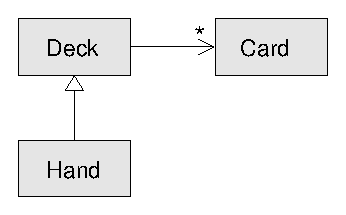
\includegraphics{figs/class1.eps}}
\afterfig

The arrow with a hollow triangle head represents an IS-A
relationship; in this case it indicates that Hand inherits
from Deck.

The standard arrow head represents a HAS-A
relationship; in this case a Deck has references to Card
objects.

\index{multiplicity (in class diagram)}

The star ({\tt *}) near the arrow head is a 
{\bf multiplicity}; it indicates how many Cards a Deck has.
A multiplicity can be a simple number, like {\tt 52}, a range,
like {\tt 5..7} or a star, which indicates that a Deck can
have any number of Cards.

A more detailed diagram might show that a Deck actually
contains a {\em list} of Cards, but built-in types
like list and dict are usually not included in class diagrams.

\begin{ex}
Read {\tt TurtleWorld.py}, {\tt World.py} and {\tt Gui.py}
and draw a class diagram that shows the relationships among
the classes defined there.
\end{ex}


\section{Debugging}
\index{debugging}

Inheritance can make debugging a challenge because when you
invoke a method on an object, you might not know which method
will be invoked.

\index{polymorphism}

Suppose you are writing a function that works with Hand objects.
You would like it to work with all kinds of Hands, like
PokerHands, BridgeHands, etc.  If you invoke a method like
{\tt shuffle}, you might get the one defined in {\tt Deck},
but if any of the subclasses override this method, you'll
get that version instead.  

\index{flow of execution}

Any time you are unsure about the flow of execution through your
program, the simplest solution is to add print statements at the
beginning of the relevant methods.  If {\tt Deck.shuffle} prints a
message that says something like {\tt Running Deck.shuffle}, then as
the program runs it traces the flow of execution.

As an alternative, you could use this function, which takes an
object and a method name (as a string) and returns the class that
provides the definition of the method:

\beforeverb
\begin{verbatim}
def find_defining_class(obj, meth_name):
    for ty in type(obj).mro():
        if meth_name in ty.__dict__:
            return ty
\end{verbatim}
\afterverb
%
Here's an example:

\beforeverb
\begin{verbatim}
>>> hand = Hand()
>>> print find_defining_class(hand, 'shuffle')
<class 'Card.Deck'>
\end{verbatim}
\afterverb
%
So the {\tt shuffle} method for this Hand is the one in {\tt Deck}.

\index{mro method}
\index{method!mro}
\index{method resolution order}

\verb"find_defining_class" uses the {\tt mro} method to get the list
of class objects (types) that will be searched for methods.  ``MRO''
stands for ``method resolution order.''

\index{override}
\index{interface}
\index{precondition}
\index{postcondition}

Here's a program design suggestion: whenever you override a method,
the interface of the new method should be the same as the old.  It
should take the same parameters, return the same type, and obey the
same preconditions and postconditions.  If you obey this rule, you
will find that any function designed to work with an instance of a
superclass, like a Deck, will also work with instances of subclasses
like a Hand or PokerHand.

If you violate this rule, your code will collapse like (sorry)
a house of cards.


\section{Glossary}

\begin{description}

\item[encode:]  To represent one set of values using another
set of values by constructing a mapping between them.
\index{encode}

\item[class attribute:] An attribute associated with a class
object.  Class attributes are defined inside
a class definition but outside any method.
\index{class attribute}
\index{attribute!class}

\item[instance attribute:] An attribute associated with an
instance of a class.
\index{instance attribute}
\index{attribute!instance}

\item[veneer:] A method or function that provides a different
interface to another function without doing much computation.
\index{veneer}

\item[inheritance:] The ability to define a new class that is a
modified version of a previously defined class.
\index{inheritance}

\item[parent class:] The class from which a child class inherits.
\index{parent class}

\item[child class:] A new class created by inheriting from an
existing class; also called a ``subclass.''
\index{child class}
\index{class!child}

\item[IS-A relationship:] The relationship between a child class
and its parent class.
\index{IS-A relationship}

\item[HAS-A relationship:] The relationship between two classes
where instances of one class contain references to instances of
the other.
\index{HAS-A relationship}

\item[class diagram:] A diagram that shows the classes in a program
and the relationships between them.
\index{class diagram}
\index{diagram!class}

\item[multiplicity:] A notation in a class diagram that shows, for
a HAS-A relationship, how many references there are to instances
of another class.
\index{multiplicity (in class diagram)}

\end{description}


\section{Exercises}

\begin{ex}
\index{poker}


The following are the possible hands in poker, in increasing order
of value (and decreasing order of probability):

\begin{description}

\item[pair:] two cards with the same rank
\vspace{-0.05in}

\item[two pair:] two pairs of cards with the same rank
\vspace{-0.05in}

\item[three of a kind:] three cards with the same rank
\vspace{-0.05in}

\item[straight:] five cards with ranks in sequence (aces can
be high or low, so {\tt Ace-2-3-4-5} is a straight and so is {\tt
10-Jack-Queen-King-Ace}, but {\tt Queen-King-Ace-2-3} is not.)
\vspace{-0.05in}

\item[flush:] five cards with the same suit
\vspace{-0.05in}

\item[full house:] three cards with one rank, two cards with another
\vspace{-0.05in}

\item[four of a kind:] four cards with the same rank
\vspace{-0.05in}

\item[straight flush:] five cards in sequence (as defined above) and
with the same suit
\vspace{-0.05in}

\end{description}
%
The goal of these exercises is to estimate
the probability of drawing these various hands.

\begin{enumerate}

\item Download the following files from \url{thinkpython.com/code}:

\begin{description}

\item[{\tt Card.py}]: A complete version of the {\tt Card},
{\tt Deck} and {\tt Hand} classes in this chapter.

\item[{\tt PokerHand.py}]: An incomplete implementation of a class
that represents a poker hand, and some code that tests it.

\end{description}
%
\item If you run {\tt PokerHand.py}, it deals seven 7-card poker hands
and checks to see if any of them contains a flush.  Read this
code carefully before you go on.

\item Add methods to {\tt PokerHand.py} named \verb"has_pair",
\verb"has_twopair", etc. that return True or False according to
whether or not the hand meets the relevant criteria.  Your code should
work correctly for ``hands'' that contain any number of cards
(although 5 and 7 are the most common sizes).

\item Write a method named {\tt classify} that figures out
the highest-value classification for a hand and sets the
{\tt label} attribute accordingly.  For example, a 7-card hand
might contain a flush and a pair; it should be labeled ``flush''.

\item When you are convinced that your classification methods are
working, the next step is to estimate the probabilities of the various
hands.  Write a function in {\tt PokerHand.py} that shuffles a deck of
cards, divides it into hands, classifies the hands, and counts the
number of times various classifications appear.

\item Print a table of the classifications and their probabilities.
Run your program with larger and larger numbers of hands until the
output values converge to a reasonable degree of accuracy.  Compare
your results to the values at \url{wikipedia.org/wiki/Hand_rankings}.

\end{enumerate}
\end{ex}


\begin{ex}

\index{Swampy}
\index{TurtleWorld}

This exercise uses TurtleWorld from Chapter~\ref{turtlechap}.
You will write code that makes Turtles play tag.  If you
are not familiar with the rules of tag, see
\url{wikipedia.org/wiki/Tag_(game)}.

\begin{enumerate}

\item Download \url{thinkpython.com/code/Wobbler.py} and run it.  You
should see a TurtleWorld with three Turtles.  If you press the
{\sf Run} button, the Turtles wander at random.

\item Read the code and make sure you understand how it works.
The {\tt Wobbler} class inherits from {\tt Turtle}, which means
that the {\tt Turtle} methods {\tt lt}, {\tt rt}, {\tt fd}
and {\tt bk} work on Wobblers.

The {\tt step} method gets invoked by TurtleWorld.  It invokes 
{\tt steer}, which turns the Turtle in the desired direction,
{\tt wobble}, which makes a random turn in proportion to the Turtle's
clumsiness, and {\tt move}, which moves forward a few pixels,
depending on the Turtle's speed.

\index{Tagger}

\item Create a file named {\tt Tagger.py}.  Import everything from
  {\tt Wobbler}, then define a class named {\tt Tagger} that inherits
  from {\tt Wobbler}.  Call \verb"make_world" passing the {\tt
    Tagger} class object as an argument.

\item Add a {\tt steer} method to {\tt Tagger} to override the one in
  {\tt Wobbler}.  As a starting place, write a version that always
  points the Turtle toward the origin.  Hint: use the math function
  {\tt atan2} and the Turtle attributes {\tt x}, {\tt y} and
  {\tt heading}.

\item Modify {\tt steer} so that the Turtles stay in bounds.
  For debugging, you might want to use the {\sf Step} button,
  which invokes {\tt step} once on each Turtle.

\item Modify {\tt steer} so that each Turtle points toward its nearest
  neighbor.  Hint: Turtles have an attribute, {\tt world}, that is a
  reference to the TurtleWorld they live in, and the TurtleWorld has
  an attribute, {\tt animals}, that is a list of all Turtles in the
  world.

\item Modify {\tt steer} so the Turtles play tag.  You can add methods
  to {\tt Tagger} and you can override {\tt steer} and
  \verb"__init__", but you may not modify or override {\tt step}, {\tt
    wobble} or {\tt move}.  Also, {\tt steer} is allowed to change the
  heading of the Turtle but not the position.

Adjust the rules and your {\tt steer} method for good quality play;
for example, it should be possible for the slow Turtle to tag the
faster Turtles eventually.

\end{enumerate}

You can get my solution from \url{thinkpython.com/code/Tagger.py}.
\end{ex}



\chapter{Case study: Tkinter}

\section{GUI}

Most of the programs we have seen so far are text-based, but
many programs use {\bf graphical user interfaces}, also
known as {\bf GUIs}.

\index{GUI}
\index{graphical user interface}
\index{Tkinter}

Python provides several choices for writing GUI-based programs,
including wxPython, Tkinter, and Qt.  Each has pros and cons, which
is why Python has not converged on a standard.

The one I will present in this chapter is Tkinter because I think
it is the easiest to get started with.  Most of the concepts
in this chapter apply to the other GUI modules, too.

There are several books and web pages about Tkinter.  One of
the best online resources is {\em An Introduction to Tkinter}
by Fredrik Lundh.

\index{Gui module}
\index{module!Gui}
\index{Swampy}

I have written a module called {\tt Gui.py} that comes with
Swampy.  It provides a simplified interface to the functions
and classes in Tkinter.  The examples in this chapter are
based on this module.

Here is a simple example that creates and displays a Gui:

To create a GUI, you have to import {\tt Gui} and instantiate
a Gui object:

\beforeverb
\begin{verbatim}
from Gui import *

g = Gui()
g.title('Gui')
g.mainloop()
\end{verbatim}
\afterverb
%
When you run this code, a window should appear with an empty gray
square and the title {\sf Gui}.  {\tt mainloop} runs the {\bf event
  loop}, which waits for the user to do something and responds
accordingly.  It is an infinite loop; it runs until the user closes
the window, or presses Control-C, or does something that causes the
program to quit.

\index{event loop}
\index{loop!event}
\index{infinite loop}
\index{loop!infinite}

This Gui doesn't do much because it doesn't have any
{\bf widgets}.  Widgets are the elements that make up a
GUI; they include:

\index{widget}

\begin{description}

\item[Button:] A widget, containing text or an image, that
performs an action when pressed.

\item[Canvas:] A region that can display lines, rectangles,
circles and other shapes.

\item[Entry:] A region where users can type text.

\item[Scrollbar:] A widget that controls the visible part of another
widget.

\item[Frame:] A container, often invisible, that contains other
widgets.

\end{description}

The empty gray square you see when you create a Gui is
a Frame.  When you create a new widget, it is added to this Frame.



\section{Buttons and callbacks}

\index{Button widget}
\index{widget!Button}

The method {\tt bu} creates a Button widget:

\beforeverb
\begin{verbatim}
button = g.bu(text='Press me.')
\end{verbatim}
\afterverb
%
The return value from {\tt bu} is a Button object.  The button
that appears in the Frame is a graphical representation of this
object; you can control the button by invoking methods on it.

\index{option}

{\tt bu} takes up to 32 parameters that control the appearance
and function of the button.  These parameters are called
{\bf options}.  Instead of providing values for all 32 options,
you can use keyword arguments, like \verb"text='Press me.'",
to specify only the options you need and use the default
values for the rest.

\index{keyword argument}
\index{argument!keyword}

When you add a widget to the Frame, it gets ``shrink-wrapped;''
that is, the Frame shrinks to the size of the Button.  If you
add more widgets, the Frame grows to accommodate them.

\index{Label widget}
\index{widget!Label}

The method {\tt la} creates a Label widget:

\beforeverb
\begin{verbatim}
label = g.la(text='Press the button.')
\end{verbatim}
\afterverb
%
By default, Tkinter stacks the widgets top-to-bottom and centers
them.  We'll see how to override that behavior soon.

If you press the button, you will see that it doesn't do much.
That's because you haven't ``wired it up;'' that is, you haven't
told it what to do!

The option that controls the behavior of a button is {\tt command}.
The value of {\tt command} is a function that gets executed when
the button is pressed.  For example, here is a function that creates
a new Label:

\beforeverb
\begin{verbatim}
def make_label():
    g.la(text='Thank you.')
\end{verbatim}
\afterverb
%
Now we can create a button with this function as its command:

\beforeverb
\begin{verbatim}
button2 = g.bu(text='No, press me!', command=make_label)
\end{verbatim}
\afterverb
%
When you press this button, it should execute \verb"make_label"
and a new label should appear.

\index{callback}

The value of the {\tt command} option
is a function object, which is known as a {\bf callback} because
after you call {\tt bu} to create the button, the flow of execution
``calls back'' when the user presses the button.

\index{event-driven programming}

This kind of flow is characteristic of {\bf event-driven programming}.
User actions, like button presses and key strokes, are called {\bf
events}.  In event-driven programming, the flow of execution is
determined by user actions rather than by the programmer.  

The challenge of event-driven programming is to construct a set of
widgets and callbacks that work correctly (or at least generate
appropriate error messages) for any sequence of user actions.

\begin{ex}
Write a program that creates a GUI with a single button.  When the
button is pressed it should create a second button.  When
{\em that} button is pressed, it should create a label that
says, ``Nice job!''.

What happens if you press the buttons more than once?
You can see my solution at \url{thinkpython.com/code/button_demo.py}

\end{ex}


\section{Canvas widgets}

\index{Canvas widget}
\index{widget!Canvas}

One of the most versatile widgets is the Canvas, which creates
a region for drawing lines, circles and other shapes.  If you
did Exercise~\ref{canvas} you are already familiar with canvases.

The method {\tt ca} creates a new Canvas:

\beforeverb
\begin{verbatim}
canvas = g.ca(width=500, height=500)
\end{verbatim}
\afterverb
%
{\tt width} and {\tt height} are the dimensions of the canvas
in pixels.  

\index{config method}
\index{method!config}

After you create a widget, you can still change the values of
the options with the
{\tt config} method.  For example, the {\tt bg} option changes
the background color:

\beforeverb
\begin{verbatim}
canvas.config(bg='white')
\end{verbatim}
\afterverb
%
The value of {\tt bg} is a string
that names a color.  The set of legal color names is different
for different implementations of Python, but all implementations
provide at least:

\beforeverb
\begin{verbatim}
white   black
red     green    blue   
cyan    yellow   magenta
\end{verbatim}
\afterverb
%
Shapes on a Canvas are called {\bf items}.  For example,
the Canvas method {\tt circle} draws (you guessed it) a circle:

\index{Canvas item}
\index{item!Canvas}

\beforeverb
\begin{verbatim}
item = canvas.circle([0,0], 100, fill='red')
\end{verbatim}
\afterverb
%
The first argument is a coordinate pair that specifies the
center of the circle; the second is the radius.

\index{Canvas coordinate}
\index{coordinate!Canvas}

{\tt Gui.py} provides a standard Cartesian coordinate system with
the origin at the center of the Canvas and the positive $y$ axis
pointing up.  This is different from some other graphics systems
where the origin is in the upper left corner, with the $y$ axis
pointing down.

The {\tt fill} option specifies that the circle should be filled
in with red.

The return value from {\tt circle} is an Item object that
provides methods for modifying the item on the canvas.  For
example, you can use {\tt config} to change any of the circle's
options:

\beforeverb
\begin{verbatim}
item.config(fill='yellow', outline='orange', width=10)
\end{verbatim}
\afterverb
%
{\tt width} is the thickness of the outline in pixels;
{\tt outline} is the color.

\begin{ex}
\label{circle}
Write a program that creates a Canvas and a Button.  When the
user presses the Button, it should draw a circle on the canvas.
\end{ex}


\section{Coordinate sequences}

\index{coordinate sequence}
\index{sequence!coordinate}

The {\tt rectangle} method takes a sequence of coordinates that
specify opposite corners of the rectangle.  This example
draws a green rectangle with the lower left corner at the origin
and the upper right corner at $(200, 100)$:

\beforeverb
\begin{verbatim}
canvas.rectangle([[0, 0], [200, 100]], 
                 fill='blue', outline='orange', width=10)
\end{verbatim}
\afterverb
%
This way of specifying corners is called
a {\bf bounding box} because the two points
bound the rectangle.

\index{bounding box}

{\tt oval} takes a bounding box and draws an oval
within the specified rectangle:

\beforeverb
\begin{verbatim}
canvas.oval([[0, 0], [200, 100]], outline='orange', width=10)
\end{verbatim}
\afterverb
%
{\tt line} takes a sequence of coordinates and draws
a line that connects the points.  This example draws two legs
of a triangle:

\beforeverb
\begin{verbatim}
canvas.line([[0, 100], [100, 200], [200, 100]], width=10)
\end{verbatim}
\afterverb
%
{\tt polygon} takes the same arguments, but it draws the last
leg of the polygon (if necessary) and fills it in:

\beforeverb
\begin{verbatim}
canvas.polygon([[0, 100], [100, 200], [200, 100]],
               fill='red', outline='orange', width=10)
\end{verbatim}
\afterverb
%


\section{More widgets}

\index{Text widget}
\index{widget!Text}

Tkinter provides two widgets that let users type text: an
Entry, which is a single line, and a Text widget, which has
multiple lines.

\index{Entry widget}
\index{widget!Entry}

{\tt en} creates a new Entry:

\beforeverb
\begin{verbatim}
entry = g.en(text='Default text.')
\end{verbatim}
\afterverb
%
The {\tt text} option allows you to put text into the entry
when it is created.  The {\tt get} method returns the contents
of the Entry (which may have been changed by the user):

\beforeverb
\begin{verbatim}
>>> entry.get()
'Default text.'
\end{verbatim}
\afterverb
%
{\tt te} creates a Text widget:

\beforeverb
\begin{verbatim}
text = g.te(width=100, height=5)
\end{verbatim}
\afterverb
%
{\tt width} and {\tt height} are the dimensions of the
widget in characters and lines.

{\tt insert} puts text into the Text widget:

\beforeverb
\begin{verbatim}
text.insert(END, 'A line of text.')
\end{verbatim}
\afterverb
%
{\tt END} is a special index that indicates the last character in the
Text widget.

You can also specify a character using a dotted index, like {\tt 1.1},
which has the line number before the dot and the column number after.
The following example adds the letters \verb"'nother'" after the first
character of the first line.

\beforeverb
\begin{verbatim}
>>> text.insert(1.1, 'nother')
\end{verbatim}
\afterverb
%
The {\tt get} method reads the text in the widget; it takes a start
and end index as arguments.  The following example returns all the
text in the widget, including the newline character:

\beforeverb
\begin{verbatim}
>>> text.get(0.0, END)
'Another line of text.\n'
\end{verbatim}
\afterverb
%
The {\tt delete} method removes text from the widget;
the following example deletes all but the first two characters:

\beforeverb
\begin{verbatim}
>>> text.delete(1.2, END)
>>> text.get(0.0, END)
'An\n'
\end{verbatim}
\afterverb
%

\begin{ex}
\label{circle2}

Modify your solution to Exercise~\ref{circle} by adding an
Entry widget and a second button.  When the user presses the
second button, it should read a color name from the Entry and
use it to change the fill color of the circle.  Use {\tt config}
to modify the existing circle; don't create a new one.

Your program should handle the case where the user tries to
change the color of a circle that hasn't been created, and
the case where the color name is invalid.

You can see my solution at \url{thinkpython.com/code/circle_demo.py}.

\end{ex}


\section{Packing widgets}

So far we have been stacking widgets in a single column, but in most
GUIs the layout is more complicated.  For example, here is a slightly
simplified version of TurtleWorld (see
Chapter~\ref{turtlechap}).

\beforefig
\centerline{
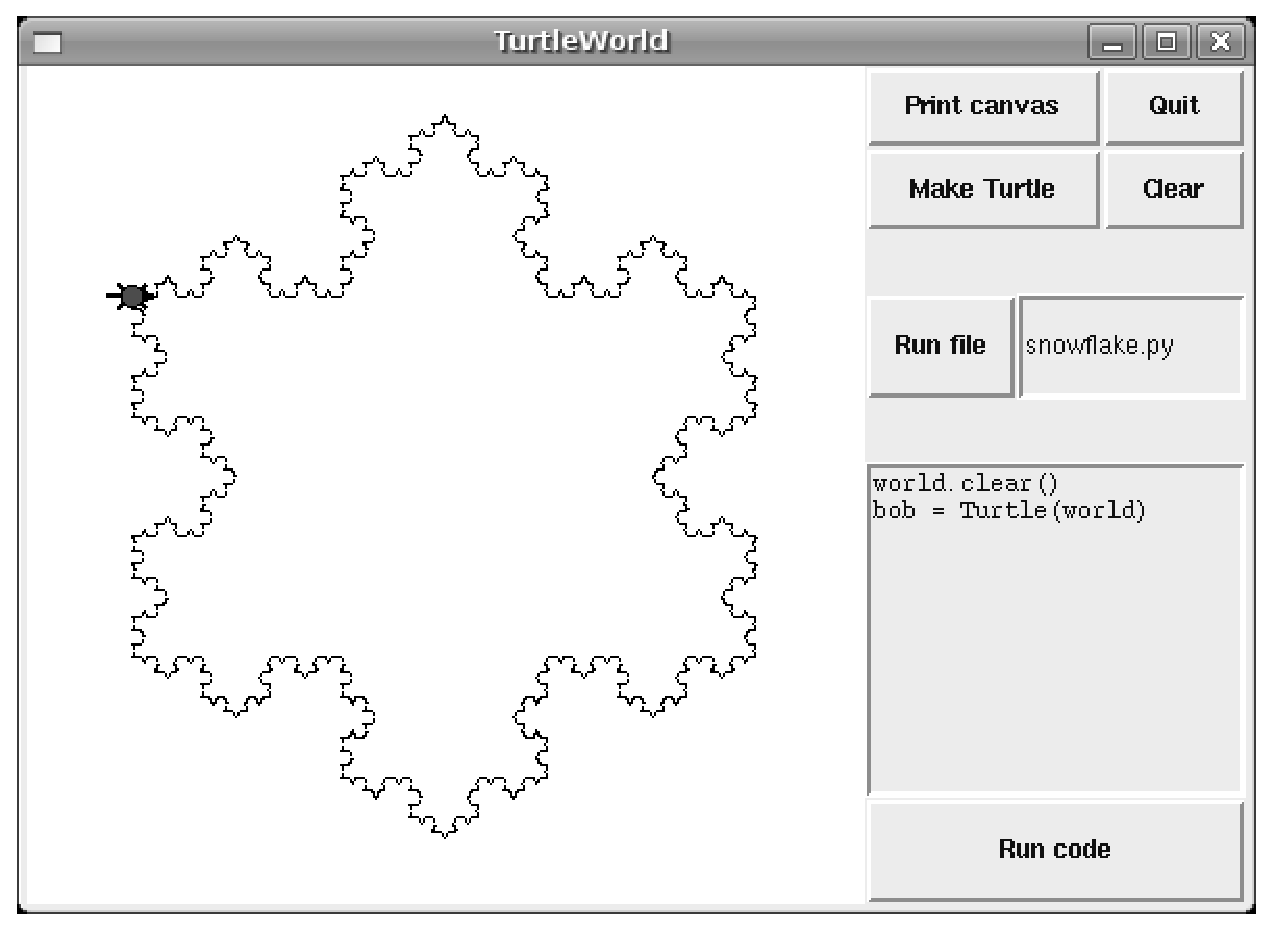
\includegraphics[width=1.0\textwidth]{figs/TurtleWorld.eps}
}
\afterfig

This section presents the code that creates this GUI, broken into a
series of steps.  You can download the complete example
from \url{thinkpython.com/code/SimpleTurtleWorld.py}.

At the top level, this GUI contains two widgets---a Canvas and a
Frame---arranged in a row.  So the first step is to create the row.

\index{SimpleTurtleWorld class}
\index{class!SimpleTurtleWorld}

\beforeverb
\begin{verbatim}
class SimpleTurtleWorld(TurtleWorld):
    """This class is identical to TurtleWorld, but the code that
    lays out the GUI is simplified for explanatory purposes."""

    def setup(self):
        self.row()
        ...
\end{verbatim}
\afterverb
%
{\tt setup} is the function that creates and arranges the widgets.
Arranging widgets in a GUI is called {\bf packing}.

\index{packing widgets}
\index{widget, packing}
\index{Frame widget}
\index{widget!Frame}

{\tt row} creates a row Frame and makes it the ``current Frame.''
Until this Frame is closed or another Frame is created, all
subsequent widgets are packed in a row.

Here is the code that creates the Canvas and the column Frame
that hold the other widgets:

\beforeverb
\begin{verbatim}
        self.canvas = self.ca(width=400, height=400, bg='white')
        self.col()
\end{verbatim}
\afterverb
%
The first widget in the column is a grid Frame, which contains
four buttons arranged two-by-two:

\beforeverb
\begin{verbatim}
        self.gr(cols=2)
        self.bu(text='Print canvas', command=self.canvas.dump)
        self.bu(text='Quit', command=self.quit)
        self.bu(text='Make Turtle', command=self.make_turtle)
        self.bu(text='Clear', command=self.clear)
        self.endgr()
\end{verbatim}
\afterverb
%
{\tt gr} creates the grid; the argument is the number of
columns.  Widgets in the grid are
laid out left-to-right, top-to-bottom.

\index{callback}
\index{bound method}
\index{method, bound}
\index{subject}

The first button uses {\tt self.canvas.dump} as a callback; the second
uses {\tt self.quit}.  These are {\bf bound methods}, which means they
are associated with a particular object.  When they are invoked, they
are invoked on the object.

The next widget in the column is a row Frame that contains
a Button and an Entry:

\beforeverb
\begin{verbatim}
        self.row([0,1], pady=30)
        self.bu(text='Run file', command=self.run_file)
        self.en_file = self.en(text='snowflake.py', width=5)
        self.endrow()
\end{verbatim}
\afterverb
%
The first argument to {\tt row} is a list of weights that
determines how extra space is allocated between widgets.  
The list {\tt [0,1]} means that all extra space is allocated
to the second widget, which is the Entry.  If you run this code
and resize the window, you will see that the Entry grows and
the Button doesn't.

The option {\tt pady} ``pads'' this row in the $y$ direction,
adding 30 pixels of space above and below.

{\tt endrow} ends this row of widgets, so subsequent widgets are
packed in the column Frame.  {\tt Gui.py} keeps a stack of Frames:

\begin{itemize}

\item When you use {\tt row}, {\tt col} or {\tt gr} to create a Frame,
it goes on top of the stack and becomes the current Frame.

\item When you use {\tt endrow}, {\tt endcol} or {\tt endgr} to close
a Frame, it gets popped off the stack and the previous Frame on the
stack becomes the current Frame.

\end{itemize} 

The method \verb"run_file" reads the contents of the Entry,
uses it as a filename, reads the contents
and passes it to \verb"run_code".  {\tt self.inter} is an
Interpreter object that knows how to take a string and
execute it as Python code.

\beforeverb
\begin{verbatim}
    def run_file(self):
        filename = self.en_file.get()
        fp = open(filename)
        source = fp.read()
        self.inter.run_code(source, filename)
\end{verbatim}
\afterverb
%
The last two widgets are a Text widget and a Button:

\beforeverb
\begin{verbatim}
        self.te_code = self.te(width=25, height=10)
        self.te_code.insert(END, 'world.clear()\n')
        self.te_code.insert(END, 'bob = Turtle(world)\n')

        self.bu(text='Run code', command=self.run_text)
\end{verbatim}
\afterverb
%
\verb"run_text" is similar to \verb"run_file" except that it takes
the code from the Text widget instead of from a file:

\beforeverb
\begin{verbatim}
    def run_text(self):
        source = self.te_code.get(1.0, END)
        self.inter.run_code(source, '<user-provided code>')
\end{verbatim}
\afterverb
%
Unfortunately, the details of widget layout are different in
other languages, and in different Python modules.
Tkinter alone provides three different mechanisms for arranging
widgets.  These mechanisms are called {\bf geometry managers}.
The one I demonstrated in this section is the ``grid'' geometry
manager; the others are called ``pack'' and ``place''.

\index{geometry manager}

Fortunately, most of the concepts in this section apply to
other GUI modules and other languages.


\section{Menus and Callables}

\index{Menubutton widget}
\index{widget!Menubutton}

A Menubutton is a widget that looks like a button, but when pressed
it pops up a menu.  After the user selects an item, the menu
disappears.

Here is code that creates a color selection Menubutton
(you can download it from \url{thinkpython.com/code/menubutton_demo.py}):

% mb_example.py

\beforeverb
\begin{verbatim}
g = Gui()
g.la('Select a color:')
colors = ['red', 'green', 'blue']
mb = g.mb(text=colors[0])
\end{verbatim}
\afterverb
%
{\tt mb} creates the Menubutton.  Initially, the text on the button is
the name of the default color.  The following loop creates one menu
item for each color:

\beforeverb
\begin{verbatim}
for color in colors:
    g.mi(mb, text=color, command=Callable(set_color, color))
\end{verbatim}
\afterverb
%
The first argument of {\tt mi} is the Menubutton these items are
associated with.

\index{callback}
\index{Callable object}
\index{object!Callable}

The {\tt command} option is a Callable object, which is something new.
So far we have seen functions and bound methods used as callbacks,
which works fine if you don't have to pass any arguments to
the function.  Otherwise you have to construct a Callable object
that contains a function, like \verb"set_color", and its arguments,
like {\tt color}.

The Callable object stores a reference to the function and the
arguments as attributes.  Later, when the user clicks on a menu
item, the callback calls the function and passes the stored
arguments.

Here is what \verb"set_color" might look like:

\beforeverb
\begin{verbatim}
def set_color(color):
    mb.config(text=color)
    print color
\end{verbatim}
\afterverb
%
When the user selects a menu item and \verb"set_color" is called,
it configures the Menubutton to display the newly-selected color.
It also print the color; if you try this example, you can confirm that
\verb"set_color" is called when you select an item (and {\em not}
called when you create the Callable object).


\section{Binding}

\index{binding}
\index{callback}

A {\bf binding} is an association between a widget, an event and a
callback: when an event (like a button press) happens on a widget, the
callback is invoked.

Many widgets have default bindings.  For example, when you press
a button, the default binding changes the relief of the button
to make it look depressed.  When you release the button, the
binding restores the appearance of the button and invokes the
callback specified with the {\tt command} option.

You can use the {\tt bind} method to override these default
bindings or to add new ones.  For example, this code creates a
binding for a canvas (you can download the code in this
section from \url{thinkpython.com/code/draggable_demo.py}):

\beforeverb
\begin{verbatim}
ca.bind('<ButtonPress-1>', make_circle)
\end{verbatim}
\afterverb
%
The first argument is an event string; this event is triggered
when the user presses the left mouse button.  Other mouse
events include {\tt ButtonMotion}, {\tt ButtonRelease} and
{\tt Double-Button}.

\index{event string}
\index{event handler}

The second argument is an event handler.  An event handler
is a function or bound method, like a callback, but an important
difference is that an event handler takes an Event object as a
parameter.  Here is an example:

\beforeverb
\begin{verbatim}
def make_circle(event):
    pos = ca.canvas_coords([event.x, event.y])
    item = ca.circle(pos, 5, fill='red')
\end{verbatim}
\afterverb
%
The Event object contains information about the type of event and
details like the coordinates of the mouse pointer.  In this example
the information we need is
the location of the mouse click.  These
values are in ``pixel coordinates,'' which are defined by the
underlying graphical system.  The method \verb"canvas_coords"
translates them to ``Canvas coordinates,'' which are compatible with
Canvas methods like {\tt circle}.

\index{Event object}
\index{object!Event}

For Entry widgets, it is common to bind the \verb"<Return>" event,
which is triggered when the user presses the {\sf Return} or
{\sf Enter} key.  For example, the following code creates a Button
and an Entry.

\beforeverb
\begin{verbatim}
bu = g.bu('Make text item:', make_text)
en = g.en()
en.bind('<Return>', make_text)
\end{verbatim}
\afterverb
%
\verb"make_text" is called when the Button is pressed or when
the user hits {\sf Return} while typing in the Entry.  To make
this work, we need a function that can be called as a command
(with no arguments) or as an event handler (with an Event
as an argument):

\beforeverb
\begin{verbatim}
def make_text(event=None):
    text = en.get()
    item = ca.text([0,0], text)
\end{verbatim}
\afterverb
%
\verb"make_text" gets the contents of the Entry and displays
it as a Text item in the Canvas.

It is also possible to create bindings for Canvas items.
The following is a class definition for {\tt Draggable},
which is a child class of {\tt Item} that provides bindings
that implement drag-and-drop capability.

\index{drag-and-drop}

\beforeverb
\begin{verbatim}
class Draggable(Item):

    def __init__(self, item):
        self.canvas = item.canvas
        self.tag = item.tag
        self.bind('<Button-3>', self.select)
        self.bind('<B3-Motion>', self.drag)
        self.bind('<Release-3>', self.drop)
\end{verbatim}
\afterverb
%
The init method takes an Item as a parameter.  It copies
the attributes of the Item and then creates bindings for
three events: a button press, button motion, and button release.

The event handler {\tt select} stores the coordinates
of the current event and the original color of the item, then
changes the color to yellow:

\beforeverb
\begin{verbatim}
    def select(self, event):
        self.dragx = event.x
        self.dragy = event.y

        self.fill = self.cget('fill')
        self.config(fill='yellow')
\end{verbatim}
\afterverb
%
{\tt cget} stands for ``get configuration;'' it takes the name of an
option as a string and returns the current value of that option.

{\tt drag} computes how far the object has moved relative to the
starting place, updates the stored coordinates, and then moves the
item.

\index{update!coordinate}

\beforeverb
\begin{verbatim}
    def drag(self, event):
        dx = event.x - self.dragx
        dy = event.y - self.dragy

        self.dragx = event.x
        self.dragy = event.y

        self.move(dx, dy)
\end{verbatim}
\afterverb
%
This computation is done in pixel coordinates; there is no need to
convert to Canvas coordinates.

\index{Canvas coordinate}
\index{coordinate!Canvas}
\index{pixel coordinate}
\index{coordinate!pixel}

Finally, {\tt drop} restores the original color of the item:

\beforeverb
\begin{verbatim}
    def drop(self, event):
        self.config(fill=self.fill)
\end{verbatim}
\afterverb
%
You can use the {\tt Draggable} class to add drag-and-drop
capability to an existing item.  For example, here is a modified
version of \verb"make_circle" that uses {\tt circle} to create
an Item and {\tt Draggable} to make it draggable:

\beforeverb
\begin{verbatim}
def make_circle(event):
    pos = ca.canvas_coords([event.x, event.y])
    item = ca.circle(pos, 5, fill='red')
    item = Draggable(item)
\end{verbatim}
\afterverb
%
This example demonstrates one of the benefits of inheritance: you can
modify the capabilities of a parent class without modifying its
definition.  This is particularly useful if you want to change
behavior defined in a module you did not write.


\section{Debugging}
\index{debugging}

One of the challenges of GUI programming is keeping track of
which things happen while the GUI is being built and which
things happen later in response to user events.

\index{callback}

For example, when you are setting up a callback, it is a common error
to call the function rather than passing a reference to it:

\beforeverb
\begin{verbatim}
def the_callback():
    print 'Called.'

g.bu(text='This is wrong!', command=the_callback())
\end{verbatim}
\afterverb
%
If you run this code, you will see that it calls \verb"the_callback"
immediately, and {\em then} creates the button.  When you press the
button, it does nothing because the return value from 
\verb"the_callback" is {\tt None}.
Usually you do not want to invoke a callback while you are
setting up the GUI; it should only be invoked later in response to
a user event.

\index{flow of execution}
\index{event-driven programming}

Another challenge of GUI programming is that you don't have control
of the flow of execution.  Which parts of the program execute
and their order are determined by user actions.
That means that you have to design your program to work correctly
for any possible sequence of events.

For example, the GUI in Exercise~\ref{circle2} has two widgets:
one creates a Circle item and the other changes the color of the
Circle.  If the user creates the circle and then changes its color,
there's no problem.  But what if the user changes the color of
a circle that doesn't exist yet?  Or creates more than one circle?

As the number of widgets grows, it is increasingly difficult to
imagine all possible sequences of events.  One way to manage this 
complexity is to encapsulate the state of the system in an object
and then consider:

\begin{itemize}

\item What are the possible states?  In the Circle example, we
might consider two states: before and after the user creates the
first circle.

\item In each state, what events can occur?  In the example,
the user can press either of the buttons, or quit.

\item For each state-event pair, what is the desired outcome?
Since there are two states and two buttons, there are four
state-event pairs to consider.

\item What can cause a transition from one state to another?
In this case, there is a transition when the user creates
the first circle.

\end{itemize}

You might also find it useful to define, and check, invariants that
should hold regardless of the sequence of events.

\index{invariant}

This approach to GUI programming can help you write correct
code without taking the time to test every possible sequence
of user events!


\section{Glossary}

\begin{description}

\item[GUI:] A graphical user interface.
\index{GUI}

\item[widget:] One of the elements that makes up a GUI, including
buttons, menus, text entry fields, etc. 
\index{widget}

\item[option:] A value that controls the appearance or function of
a widget.
\index{option}

\item[keyword argument:] An argument that indicates the parameter
name as part of the function call.
\index{keyword argument}

\item[callback:] A function associated with a widget that is
called when the user performs an action.
\index{callback}

\item[bound method:] A method associated with a particular instance.
\index{bound method}

\item[event-driven programming:] A style of programming in which
the flow of execution is determined by user actions.
\index{event-driven programming}

\item[event:] A user action, like a mouse click or key press, that
causes a GUI to respond.
\index{event}

\item[event loop:] An infinite loop that waits for user actions
and responds.
\index{event loop}

\item[item:] A graphical element on a Canvas widget.
\index{item!Canvas}

\item[bounding box:] A rectangle that encloses a set of items,
usually specified by two opposing corners.
\index{bounding box}

\item[pack:] To arrange and display the elements of a GUI.
\index{packing widgets}

\item[geometry manager:] A system for packing widgets.
\index{geometry manager}

\item[binding:] An association between a widget, an event, and
an event handler.  The event handler is called when the event
occurs in the widget.
\index{binding}

\end{description}


\section{Exercises}

\begin{ex}
\index{image viewer}

For this exercise, you will write an image viewer.  Here is
a simple example:

\beforeverb
\begin{verbatim}
g = Gui()
canvas = g.ca(width=300)
photo = PhotoImage(file='danger.gif')
canvas.image([0,0], image=photo)
g.mainloop()
\end{verbatim}
\afterverb
%
{\tt PhotoImage} reads a file and returns a {\tt PhotoImage} object
that Tkinter can display.  {\tt Canvas.image} puts the image on the
canvas, centered on the given coordinates.  You can also put images on
labels, buttons, and some other widgets:

\beforeverb
\begin{verbatim}
g.la(image=photo)
g.bu(image=photo)
\end{verbatim}
\afterverb
%
PhotoImage can only handle a few image formats, like GIF and PPM, 
but we can use the Python Imaging Library (PIL) to read other
files.

\index{Python Imaging Library (PIL)}
\index{PIL (Python Imaging Library)}
\index{Image module}
\index{module!Image}

The name of the PIL module is {\tt Image}, but Tkinter defines an
object with the same name.  To avoid the conflict, you can use {\tt
  import...as} like this:

\beforeverb
\begin{verbatim}
import Image as PIL
import ImageTk
\end{verbatim}
\afterverb
%
The first line imports {\tt Image} and
gives it the local name {\tt PIL}.  The second
line imports {\tt ImageTk}, which can translate a PIL
image into a Tkinter PhotoImage.  Here's an example:

\beforeverb
\begin{verbatim}
image = PIL.open('allen.png')
photo2 = ImageTk.PhotoImage(image)
g.la(image=photo2)
\end{verbatim}
\afterverb
%

\begin{enumerate}

\item Download \verb"image_demo.py", \verb"danger.gif" and \verb"allen.png"
from \url{thinkpython.com/code}.  Run \verb"image_demo.py".  You
might have to install {\tt PIL} and {\tt ImageTk}.  
They are probably in your software repository,  but if not
you can get them from \url{pythonware.com/products/pil/}.

\item In \verb"image_demo.py" change the name of the second
PhotoImage from {\tt photo2} to {\tt photo} and run the program
again.  You should see the second PhotoImage but not the first.

The problem is that when you reassign {\tt photo} it overwrites
the reference to the first PhotoImage, which then disappears.  The
same thing happens if you assign a PhotoImage to a local
variable; it disappears when the function ends.

To avoid this problem, you have to store a reference to each
PhotoImage you want to keep.  You can use a global variable, or
store PhotoImages in a data structure or as an attribute of
an object.

This behavior can be frustrating, which is why I am warning
you (and why the example image says ``Danger!'').

\index{bug!worst ever}
\index{worst bug!ever}

\item Starting with this example, write a program that takes
the name of a directory and loops through all the files, displaying
any files that PIL recognizes as images.  You can use a {\tt try}
statement to catch the files PIL doesn't recognize.

When the user clicks on the image, the program should display the next one.

\item PIL provides a variety of methods for manipulating images.
You can read about them at \url{pythonware.com/library/pil/handbook}.
As a challenge, choose a few of these methods and provide a
GUI for applying them to images.

\end{enumerate}

You can download a simple solution from
\url{thinkpython.com/code/ImageBrowser.py}.

\end{ex}


\begin{ex}

\index{vector graphics}
\index{SVG}

A vector graphics editor is a program that allows users to draw and
edit shapes on the screen and generate output files in vector graphics
formats like Postscript and SVG\footnote{See
  \url{wikipedia.org/wiki/Vector_graphics_editor}.}.

Write a simple vector graphics editor using Tkinter.  At a
minimum, it should allow users to draw lines, circles and
rectangles, and it should use {\tt Canvas.dump} to
generate a Postscript description of the contents of the
Canvas.

As a challenge, you could allow users to select and resize
items on the Canvas.

\end{ex}


\begin{ex}

Use Tkinter to write a basic web browser.  It
should have a Text widget where the user can enter a URL
and a Canvas to display the contents of the page.

\index{urllib module}
\index{module!urllib}
\index{URL}
\index{HTMLParser module}
\index{module!HTMLParser}

You can use the {\tt urllib} module to download files
(see Exercise~\ref{urllib}) and
the {\tt HTMLParser} module to parse the HTML
tags (see \url{docs.python.org/lib/module-HTMLParser.html}).

\index{plain text}
\index{text!plain}
\index{hyperlink}

At a minimum your browser should handle plain text and hyperlinks.  As
a challenge you could handle background colors, text
formatting tags and images.

\end{ex}



\appendix

\chapter{Debugging}
\index{debugging}

Different kinds of errors can occur
in a program, and it is useful to distinguish among them
in order to track them down more quickly:

\begin{itemize}

\item Syntax errors are produced by Python when it is translating the
  source code into byte code.  They usually indicate that there is
  something wrong with the syntax of the program.  Example: Omitting
  the colon at the end of a {\tt def} statement yields the somewhat
  redundant message {\tt SyntaxError: invalid syntax}.

\item Runtime errors are produced by the interpreter if something goes
  wrong while the program is running.  Most runtime error messages
  include information about where the error occurred and what
  functions were executing.  Example: An infinite recursion eventually
  causes the runtime error ``maximum recursion depth exceeded.''

\item Semantic errors are problems with a program that runs without
  producing error messages but doesn't do the right thing.  Example:
  An expression may not be evaluated in the order you expect, yielding
  an incorrect result.

\end{itemize}

\index{syntax error}
\index{runtime error}
\index{semantic error}
\index{error!compile-time}
\index{error!syntax}
\index{error!runtime}
\index{error!semantic}
\index{exception}

The first step in debugging is to figure out which kind of
error you are dealing with.  Although the following sections are
organized by error type, some techniques are
applicable in more than one situation.


\section{Syntax errors}

\index{error message}

Syntax errors are usually easy to fix once you figure out what they
are.  Unfortunately, the error messages are often not helpful.
The most common messages are {\tt SyntaxError: invalid syntax} and
{\tt SyntaxError: invalid token}, neither of which is very informative.

On the other hand, the message does tell you where in the program the
problem occurred.  Actually, it tells you where Python
noticed a problem, which is not necessarily where the error
is.  Sometimes the error is prior to the location of the error
message, often on the preceding line.

\index{incremental development}
\index{development plan!incremental}

If you are building the program incrementally, you should have
a good idea about where the error is.  It will be in the last
line you added.

If you are copying code from a book, start by comparing
your code to the book's code very carefully.  Check every character.
At the same time, remember that the book might be wrong, so
if you see something that looks like a syntax error, it might be.

Here are some ways to avoid the most common syntax errors:

\index{syntax}

\begin{enumerate}

\item Make sure you are not using a Python keyword for a variable name.

\index{keyword}

\item Check that you have a colon at the end of the header of every
compound statement, including {\tt for}, {\tt while},
{\tt if}, and {\tt def} statements.

\index{header}
\index{colon}

\item Make sure that any strings in the code have matching
quotation marks.

\index{quotation mark}

\item If you have multiline strings with triple quotes (single or double), make
sure you have terminated the string properly.  An unterminated string
may cause an {\tt invalid token} error at the end of your program,
or it may treat the following part of the program as a string until it
comes to the next string.  In the second case, it might not produce an error
message at all!

\index{multiline string}
\index{string!multiline}

\item An unclosed opening operator---\verb+(+, \verb+{+, or
  \verb+[+---makes Python continue with the next line as part of the
  current statement.  Generally, an error occurs almost immediately in
  the next line.

\item Check for the classic {\tt =} instead of {\tt ==} inside
a conditional.

\index{conditional}

\item Check the indentation to make sure it lines up the way it
is supposed to.  Python can handle space and tabs, but if you mix
them it can cause problems.  The best way to avoid this problem
is to use a text editor that knows about Python and generates
consistent indentation.

\index{indentation}
\index{whitespace}

\end{enumerate}

If nothing works, move on to the next section...


\subsection{I keep making changes and it makes no difference.}

If the interpreter says there is an error and you don't see it, that
might be because you and the interpreter are not looking at the same
code.  Check your programming environment to make sure that the
program you are editing is the one Python is trying to run.

If you are not sure, try putting an obvious and deliberate syntax
error at the beginning of the program.  Now run it again.  If the
interpreter doesn't find the new error, you are not running the
new code.

There are a few likely culprits:

\begin{itemize}

\item You edited the file and forgot to save the changes before
running it again.  Some programming environments do this
for you, but some don't.

\item You changed the name of the file, but you are still running
the old name.

\item Something in your development environment is configured
incorrectly.

\item If you are writing a module and using {\tt import},
make sure you don't give your module the same name as one
of the standard Python modules.

\index{module!reload}
\index{reload function}
\index{function!reload}

\item If you are using {\tt import} to read a module, remember
that you have to restart the interpreter or use {\tt reload}
to read a modified file.  If you import the module again, it
doesn't do anything.

\end{itemize}

If you get stuck and you can't figure out what is going on, one
approach is to start again with a new program like ``Hello, World!,''
and make sure you can get a known program to run.  Then gradually add
the pieces of the original program to the new one.


\section{Runtime errors}

Once your program is syntactically correct,
Python can compile it and at least start running it.  What could
possibly go wrong?


\subsection{My program does absolutely nothing.}

This problem is most common when your file consists of functions and
classes but does not actually invoke anything to start execution.
This may be intentional if you only plan to import this module to
supply classes and functions.

If it is not intentional, make sure that you
are invoking a function to start execution, or execute one from
the interactive prompt.  Also see the ``Flow of Execution'' section
below.


\subsection{My program hangs.}
\index{infinite loop}
\index{infinite recursion}
\index{hanging}

If a program stops and seems to be doing nothing, it is ``hanging.''
Often that means that it is caught in an infinite loop or infinite
recursion.

\begin{itemize}

\item If there is a particular loop that you suspect is the
problem, add a {\tt print} statement immediately before the loop that says
``entering the loop'' and another immediately after that says
``exiting the loop.''

Run the program.  If you get the first message and not the second,
you've got an infinite loop.  Go to the ``Infinite Loop'' section
below.

\item Most of the time, an infinite recursion will cause the program
to run for a while and then produce a ``RuntimeError: Maximum
recursion depth exceeded'' error.  If that happens, go to the
``Infinite Recursion'' section below.

If you are not getting this error but you suspect there is a problem
with a recursive method or function, you can still use the techniques
in the ``Infinite Recursion'' section.

\item If neither of those steps works, start testing other
loops and other recursive functions and methods.

\item If that doesn't work, then it is possible that
you don't understand the flow of execution in your program.
Go to the ``Flow of Execution'' section below.

\end{itemize}


\subsubsection{Infinite Loop}
\index{infinite loop}
\index{loop!infinite}
\index{condition}
\index{loop!condition}

If you think you have an infinite loop and you think you know
what loop is causing the problem, add a {\tt print} statement at
the end of the loop that prints the values of the variables in
the condition and the value of the condition.

For example:

\beforeverb
\begin{verbatim}
while x > 0 and y < 0 :
    # do something to x
    # do something to y

    print  "x: ", x
    print  "y: ", y
    print  "condition: ", (x > 0 and y < 0)
\end{verbatim}
\afterverb
%
Now when you run the program, you will see three lines of output
for each time through the loop.  The last time through the
loop, the condition should be {\tt false}.  If the loop keeps
going, you will be able to see the values of {\tt x} and {\tt y},
and you might figure out why they are not being updated correctly.


\subsubsection{Infinite Recursion}
\index{infinite recursion}
\index{recursion!infinite}

Most of the time, an infinite recursion will cause the program to run
for a while and then produce a {\tt Maximum recursion depth exceeded}
error.

If you suspect that a function or method is causing an infinite
recursion, start by checking to make sure that there is a base case.
In other words, there should be some condition that will cause the
function or method to return without making a recursive invocation.
If not, then you need to rethink the algorithm and identify a base
case.

If there is a base case but the program doesn't seem to be reaching
it, add a {\tt print} statement at the beginning of the function or method
that prints the parameters.  Now when you run the program, you will see
a few lines of output every time the function or method is invoked,
and you will see the parameters.  If the parameters are not moving
toward the base case, you will get some ideas about why not.


\subsubsection{Flow of Execution}
\index{flow of execution}

If you are not sure how the flow of execution is moving through
your program, add {\tt print} statements to the beginning of each
function with a message like ``entering function {\tt foo},'' where
{\tt foo} is the name of the function.

Now when you run the program, it will print a trace of each
function as it is invoked.


\subsection{When I run the program I get an exception.}
\index{exception}
\index{runtime error}

If something goes wrong during runtime, Python
prints a message that includes the name of the
exception, the line of the program where the problem occurred,
and a traceback.

\index{traceback}

The traceback identifies the function that is currently running,
and then the function that invoked it, and then the function that
invoked {\em that}, and so on.  In other words, it traces the
sequence of function invocations that got you to where you are.  It
also includes the line number in your file where each of these
calls occurs.

The first step is to examine the place in the program where
the error occurred and see if you can figure out what happened.
These are some of the most common runtime errors:

\begin{description}

\item[NameError:]  You are trying to use a variable that doesn't
exist in the current environment.
Remember that local variables are local.  You
cannot refer to them from outside the function where they are defined.

\index{NameError}
\index{TypeError}
\index{exception!NameError}
\index{exception!TypeError}

\item[TypeError:] There are several possible causes:

\begin{itemize}

\item  You are trying to use a value improperly.  Example: indexing
a string, list, or tuple with something other than an integer.

\index{index}

\item There is a mismatch between the items in a format string and
the items passed for conversion.  This can happen if either the number
of items does not match or an invalid conversion is called for.

\index{format operator}
\index{operator!format}

\item You are passing the wrong number of arguments to a function or method.
For methods, look at the method definition and
check that the first parameter is {\tt self}.  Then look at the
method invocation; make sure you are invoking the method on an
object with the right type and providing the other arguments
correctly.

\end{itemize}

\item[KeyError:]  You are trying to access an element of a dictionary
using a key that the dictionary does not contain.

\index{KeyError}
\index{exception!KeyError}
\index{dictionary}

\item[AttributeError:] You are trying to access an attribute or method
that does not exist.  Check the spelling!  You can use
{\tt dir} to list the attributes that do exist.

If an AttributeError indicates that an object has {\tt NoneType},
that means that it is {\tt None}.  One common cause is forgetting
to return a value from a function; if you get to the end of
a function without hitting a {\tt return} statement, it returns
{\tt None}.  Another common cause is using the result from
a list method, like {\tt sort}, that returns {\tt None}.

\index{AttributeError}
\index{exception!AttributeError}

\item[IndexError:] The index you are using
to access a list, string, or tuple is greater than
its length minus one.  Immediately before the site of the error,
add a {\tt print} statement to display
the value of the index and the length of the array.
Is the array the right size?  Is the index the right value?

\index{IndexError}
\index{exception!IndexError}

\end{description}

\index{debugger (pdb)}
\index{Python debugger (pdb)}
\index{pdb (Python debugger)}

The Python debugger ({\tt pdb}) is useful for tracking down
Exceptions because it allows you to examine the state of the
program immediately before the error.  You can read
about {\tt pdb} at \url{docs.python.org/lib/module-pdb.html}.


\subsection{I added so many {\tt print} statements I get inundated with
output.}

\index{print statement}
\index{statement!print}

One of the problems with using {\tt print} statements for debugging
is that you can end up buried in output.  There are two ways
to proceed: simplify the output or simplify the program.

To simplify the output, you can remove or comment out {\tt print}
statements that aren't helping, or combine them, or format
the output so it is easier to understand.

To simplify the program, there are several things you can do.  First,
scale down the problem the program is working on.  For example, if you
are searching a list, search a {\em small} list.  If the program takes
input from the user, give it the simplest input that causes the
problem.

\index{dead code}

Second, clean up the program.  Remove dead code and reorganize the
program to make it as easy to read as possible.  For example, if you
suspect that the problem is in a deeply nested part of the program,
try rewriting that part with simpler structure.  If you suspect a
large function, try splitting it into smaller functions and testing them
separately.

\index{testing!minimal test case}
\index{test case, minimal}

Often the process of finding the minimal test case leads you to the
bug.  If you find that a program works in one situation but not in
another, that gives you a clue about what is going on.

Similarly, rewriting a piece of code can help you find subtle
bugs.  If you make a change that you think shouldn't affect the
program, and it does, that can tip you off.


\section{Semantic errors}
\index{semantic error}
\index{error!semantic}

In some ways, semantic errors are the hardest to debug,
because the interpreter provides no information
about what is wrong.  Only you know what the program is supposed to
do.

The first step is to make a connection between the program
text and the behavior you are seeing.  You need a hypothesis
about what the program is actually doing.  One of the things
that makes that hard is that computers run so fast.

You will often wish that you could slow the program down to human
speed, and with some debuggers you can.  But the time it takes to
insert a few well-placed {\tt print} statements is often short compared to
setting up the debugger, inserting and removing breakpoints, and
``stepping'' the program to where the error is occurring.

\subsection{My program doesn't work.}

You should ask yourself these questions:

\begin{itemize}

\item Is there something the program was supposed to do but
which doesn't seem to be happening?  Find the section of the code
that performs that function and make sure it is executing when
you think it should.

\item Is something happening that shouldn't?  Find code in
your program that performs that function and see if it is
executing when it shouldn't.

\item Is a section of code producing an effect that is not
what you expected?  Make sure that you understand the code in
question, especially if it involves invocations to functions or methods in
other OCaml modules.  Read the documentation for the functions you invoke.
Try them out by writing simple test cases and checking the results.

\end{itemize}

In order to program, you need to have a mental model of how
programs work.  If you write a program that doesn't do what you expect,
very often the problem is not in the program; it's in your mental
model.

\index{model, mental}
\index{mental model}

The best way to correct your mental model is to break the program
into its components (usually the functions and methods) and test
each component independently.  Once you find the discrepancy
between your model and reality, you can solve the problem.

Of course, you should be building and testing components as you
develop the program.  If you encounter a problem,
there should be only a small amount of new code
that is not known to be correct.


\subsection{I've got a big hairy expression and it doesn't
do what I expect.}

\index{expression!big and hairy}
\index{big, hairy expression}

Writing complex expressions is fine as long as they are readable,
but they can be hard to debug.  It is often a good idea to
break a complex expression into a series of assignments to
temporary variables.

For example:

\beforeverb
\begin{verbatim}
self.hands[i].addCard(self.hands[self.findNeighbor(i)].popCard())
\end{verbatim}
\afterverb
%
This can be rewritten as:

\beforeverb
\begin{verbatim}
neighbor = self.findNeighbor(i)
pickedCard = self.hands[neighbor].popCard()
self.hands[i].addCard(pickedCard)
\end{verbatim}
\afterverb
%
The explicit version is easier to read because the variable
names provide additional documentation, and it is easier to debug
because you can check the types of the intermediate variables
and display their values.

\index{temporary variable}
\index{variable!temporary}
\index{order of operations}
\index{precedence}

Another problem that can occur with big expressions is
that the order of evaluation may not be what you expect.
For example, if you are translating the expression
$\frac{x}{2 \pi}$ into Python, you might write:

\beforeverb
\begin{verbatim}
y = x / 2 * math.pi
\end{verbatim}
\afterverb
%
That is not correct because multiplication and division have
the same precedence and are evaluated from left to right.
So this expression computes $x \pi / 2$.

A good way to debug expressions is to add parentheses to make
the order of evaluation explicit:

\beforeverb
\begin{verbatim}
 y = x / (2 * math.pi)
\end{verbatim}
\afterverb
%
Whenever you are not sure of the order of evaluation, use
parentheses.  Not only will the program be correct (in the sense
of doing what you intended), it will also be more readable for
other people who haven't memorized the rules of precedence.


\subsection{I've got a function or method that doesn't return what I
expect.}
\index{return statement}
\index{statement!return}

If you have a {\tt return} statement with a complex expression,
you don't have a chance to print the {\tt return} value before
returning.  Again, you can use a temporary variable.  For
example, instead of:

\beforeverb
\begin{verbatim}
return self.hands[i].removeMatches()
\end{verbatim}
\afterverb
%
you could write:

\beforeverb
\begin{verbatim}
count = self.hands[i].removeMatches()
return count
\end{verbatim}
\afterverb
%
Now you have the opportunity to display the value of
{\tt count} before returning.


\subsection{I'm really, really stuck and I need help.}

First, try getting away from the computer for a few minutes.
Computers emit waves that affect the brain, causing these
symptoms:

\begin{itemize}

\item Frustration and rage.

\index{frustration}
\index{rage}
\index{debugging!emotional response}
\index{emotional debugging}

\item Superstitious beliefs (``the computer hates me'') and
magical thinking (``the program only works when I wear my
hat backward'').

\index{debugging!superstition}
\index{superstitious debugging}

\item Random walk programming (the attempt to program by writing
every possible program and choosing the one that does the right
thing).

\index{random walk programming}
\index{development plan!random walk programming}

\end{itemize}

If you find yourself suffering from any of these symptoms, get
up and go for a walk.  When you are calm, think about the program.
What is it doing?  What are some possible causes of that
behavior?  When was the last time you had a working program,
and what did you do next?

Sometimes it just takes time to find a bug.  I often find bugs
when I am away from the computer and let my mind wander.  Some
of the best places to find bugs are trains, showers, and in bed,
just before you fall asleep.


\subsection{No, I really need help.}

It happens.  Even the best programmers occasionally get stuck.
Sometimes you work on a program so long that you can't see the
error.  A fresh pair of eyes is just the thing.

Before you bring someone else in, make sure you are prepared.
Your program should be as simple
as possible, and you should be working on the smallest input
that causes the error.  You should have {\tt print} statements in the
appropriate places (and the output they produce should be
comprehensible).  You should understand the problem well enough
to describe it concisely.

When you bring someone in to help, be sure to give
them the information they need:

\begin{itemize}

\item If there is an error message, what is it
and what part of the program does it indicate?

\item What was the last thing you did before this error occurred?
What were the last lines of code that you wrote, or what is
the new test case that fails?

\item What have you tried so far, and what have you learned?

\end{itemize}

When you find the bug, take a second to think about what you
could have done to find it faster.  Next time you see something
similar, you will be able to find the bug more quickly.

Remember, the goal is not just to make the program
work.  The goal is to learn how to make the program work.



\printindex

\clearemptydoublepage
%\blankpage
%\blankpage
%\blankpage


\end{document}
